% -----------------------------------------------------------------
% Vorlage fuer Ausarbeitungen von
% Bachelor- und Masterarbeiten am ISS
% 
% Template for written reports or master theses at the ISS
% 
% For use with compilers pdflatex or latex->dvi2ps->ps2pdf.
%
% -----------------------------------------------------------------
% README, STUDENT USERS:
% We highly appreciate students using this template _AS IS_,period. 
% The document provides adjustable document preferences, 
% student information settings and typography definitions. Look for
% code delimited by *** ***
%
% The short explanation: it's the ISS common standard and 
% 	it's battle tested.
% The long explanation: 
%	We do not want you to go through the document and tweak the 
%	package options, layout parameters and line skips here and 
%	there and waste hours. We are providing this template such 
%	that you can fully concentrate on filling in the much more 
%	important _contents_ of your thesis.
%
% If you have serious needs on extra packages or design 
% modifications, talk to your supervisor _before_ modifying 
% the template.
% Similarly, we're happy if you give your supervisor a hint on any 
% errors in this template.
%
% -----------------------------------------------------------------
% History:
% Jan Scheuing,   04.03.2002
% Markus Buehren, 20.12.2004
% last changes:   10.01.2008 (removed unused packages), 
% 		07.08.2009 (added IEEEtran_LSS.bst file)
% 		02.05.2011 removed matriculation number from cover page
% Martin Kreissig, 25.01.2012: all eps/ps parts removed for 
% 				pdflatex to work properly
% Peter Hermannstaedter, 14.08.2012: fusion of versions for 
% 		latex/dvi/ps/pdf and pdflatex, additional comments,
% 		unification of document flags and student options
% Florian Liebgott, 12.03.2015: bug fixes, removal of obsolete options,
%		switch to UTF-8
% Florian Liebgott, 20.05.2015: fixed encoding problem on title page
% Florian Liebgott, 24.01.2017: changed deprecated font commands (like
%		\sl) to up-to-date commands to be compatible with
%		current TeX distributions.
% Felix Wiewel, 30.08.2021: Replace obsolete scrpage2 with scrlayer-scrpage
%
% -----------------------------------------------------------------
% If you experience any errors caused by this template, please
% contact Florian Liebgott (florian.liebgott@iss.uni-stuttgart.de)
% or your supervisor, so we can fix the errors.
% -----------------------------------------------------------------


\documentclass[12pt,DIV14,BCOR12mm,a4paper,footinclude=false,headinclude,parskip=half-,twoside,openright,cleardoublepage=empty,toc=index,bibliography=totoc,listof=totoc]{scrreprt}
% encoding needs to be defined here, otherwise umlauts on the titelpage won't work.
\usepackage[utf8]{inputenc}
%
%
%
% *****************************************************************
% -------------------> document preferences here <-----------------
% *****************************************************************
% Uncomment the settings you like and comment the settings you don't
% like.

% Language: 
% affects generic titles, Figure term, titlepage and bibliography
% (Note:if you switch the language, compile tex and bib >2 times)
\def \doclang{english} 	% For theses/reports in English
%\def \doclang{german} 		% For theses/reports in German

% Hyperref links in the document:
\def \colortype{color} % links with colored text
%\def \colortype{bw} 	% plain links, standard text color (e.g. for print)
%\def \colortype{boxed} % links with colored boxes
% *****************************************************************
%
%
%
% *****************************************************************
% --------------> put student information here <------------------
% *****************************************************************
% Please fill in all items denoted by "to be defined (TBD)"
\def \deworktitle{Schätzung der 6-DoF-Pose mit Diffusion Modelle aus einem einzelnen RGB-D-Bild}        % German title/translation
\def \enworktitle{6 DoF Pose Estimation with Diffusion Models from a Single RGB-D Image}        % English title/translation
\def \tutor{Junwen Huang}
\def \student{Haoqing Wu}
\def \worksubject{Master's Thesis D1475}  % type and number (S/Dxxxx) of your thesis
\def \startdate{01.06.2023}
\def \submission{30.11.2023}
\def \signagedate{30.11.2023}   % Date of signature of declaration on last page
\def \keywords{Deep Learning, Computer Vision, 6 DoF Pose Estimation, Diffusion Probabilistic Models}
\def \abstract{
  6 DoF pose estimation, a crucial aspect in the realms of computer vision and robotics, has witnessed considerable attention, particularly with the advent of deep learning methodologies. Recent years have seen the emergence of diverse techniques, encompassing RGB-based methods, depth-focused approaches and RGB-D fusion, aimed at enhancing the accuracy of pose estimation. However, challenges persist in scenarios involving textureless objects, occlusion, and cluttered backgrounds. This thesis introduces a pioneering pose estimation method founded on diffusion models, which have demonstrated notable success in image synthesis tasks. The objective is to leverage the strengths of diffusion models, such as their scalability to large-scale data and the diversity of generation, to address the complexities inherent in 6 DoF pose estimation. A comprehensive diffusion framework is proposed, utilizing a single RGB-D image to generate multiple hypotheses for the 6 DoF pose of an object. The proposed method is rigorously evaluated on real-world datasets featuring noise and occlusion. Results indicate that our approach achieves comparable performance with state-of-the-art methods, highlighting its effectiveness in challenging scenarios. This study not only contributes a novel perspective to pose estimation but also underscores the potential of diffusion models in advancing the state of the art in this critical domain.
  \newline
  \newline
  \newline
  Schätzung der 6-DoF-Pose, ein entscheidender Aspekt in den Bereichen Computer Vision und Robotik, hat erhebliche Aufmerksamkeit erfahren, insbesondere mit dem Aufkommen von Deep Learning Methoden. In den letzten Jahren sind verschiedene Techniken aufgetaucht, darunter RGB-basierte Methoden, auf Tiefen fokussierte Ansätze und RGB-D Fusion, die darauf abzielen, die Genauigkeit der Schätzung zu verbessern. Herausforderungen bleiben jedoch in Szenarien mit strukturlosen Objekten, Okklusion und überladenem Hintergrund bestehen. Diese Arbrit stellt eine bahnbrechende Pose-Schätzungsmethode auf Grundlage von Diffusionsmodellen vor, die in Bildsyntheseaufgaben bemerkenswerte Erfolge gezeigt haben. Das Ziel besteht darin, die Stärken der Diffusionsmodelle, wie ihre Skalierbarkeit für große Datenmengen und die Vielfalt der Generierung, zu nutzen, um den in der 6-DoF-Pose-Schätzung inhärenten Komplexitäten zu begegnen. Es wird ein umfassender Diffusionsrahmen vorgeschlagen, der ein einzelnes RGB-D-Bild verwendet, um mehrere Hypothesen für die 6-DoF-Pose eines Objekts zu generieren. Die vorgeschlagene Methode wird sorgfältig an realen Datensätzen mit Rauschen und Okklusion evaluiert. Die Ergebnisse zeigen, dass unser Ansatz vergleichbare Leistungen mit modernsten Methoden erreicht, was seine Effektivität in anspruchsvollen Szenarien unterstreicht. Diese Studie trägt nicht nur eine neue Perspektive zur Pose-Schätzung bei, sondern betont auch das Potenzial der Diffusionsmodelle zur Weiterentwicklung des State-of-the-Art in diesem kritischen Bereich.
}

% *****************************************************************
%


\usepackage{amsmath}
\usepackage{amsfonts}
\usepackage{ifthen}
\ifthenelse{\equal{\doclang}{german}}{
	\usepackage[ngerman]{babel} %german version
	\def \maintitle{\deworktitle}
	\def \translatedtitle{\enworktitle}
	% set , to decimal and . to thousands separator, if German language is used
	\DeclareMathSymbol{,}{\mathord}{letters}{"3B}
	\DeclareMathSymbol{.}{\mathpunct}{letters}{"3A}
	}{
	%english version
	\def \maintitle{\enworktitle}
	\def \translatedtitle{\deworktitle}
	}
\usepackage{txfonts} % Times-Fonts
\usepackage[T1]{fontenc}
\usepackage{color}
\usepackage[headsepline]{scrlayer-scrpage} % Headings

\usepackage{graphicx}
\usepackage[format=hang]{caption}       % for hanging captions
\usepackage{subfig}                     % for subfigures
\usepackage{wrapfig}                    % for figures floating in text, alternatively you can use >>floatflt<<
\usepackage{booktabs}                   % nice looking tables (for tables with ONLY horizontal lines)
\usepackage{algorithm}                  % for pseudocode
\usepackage{algorithmicx}                % for pseudocode
\usepackage{algpseudocode}              % for pseudocode
\usepackage[export]{adjustbox}
\usepackage{epsfig}
\usepackage{array}
\usepackage[acronym,automake]{glossaries}
\usepackage{nomencl}
\usepackage{etoolbox}
\usepackage{multirow}
\usepackage{anyfontsize}

%%%%% Tikz / PGF - drawing beautiful graphics and plots in Latex
% \usepackage{tikz}
% \usetikzlibrary{plotmarks}              % larger choice of plot marks
% \usetikzlibrary{arrows}                 % larger choice of arrow heads
% % ... insert other libraries you need
% \usepackage{pgfplots}
% % set , to decimal and . to thousands separator for plots, if German language is used
% \ifthenelse{\equal{\doclang}{german}}{
% \pgfkeys{/pgf/number format/set decimal separator={,}}
% \pgfkeys{/pgf/number format/set thousands separator={.}}
% }{}
%%%%%%

\ifthenelse{\equal{\colortype}{color}}{
	% colored text version:
	\usepackage[colorlinks,linkcolor=blue]{hyperref}
	\newcommand{\bugfix}{\color{white}{\texttt{\symbol{'004}}}} % Bug-Fix Umlaute in Verbatim
}{
	\ifthenelse{\equal{\colortype}{boxed}}{
		% colored box version:
		\usepackage{hyperref}
		\newcommand{\bugfix}{\color{white}{\texttt{\symbol{'004}}}} % Bug-Fix Umlaute in Verbatim
	}{
		% monochrome version:
		\usepackage[hidelinks]{hyperref}
		\newcommand{\bugfix}{\color{white}{\texttt{\symbol{'004}}}} % Bug-Fix Umlaute in Verbatim
	}
}

% Layout and Headings
\pagestyle{scrheadings}
\automark{chapter}
\clearscrheadfoot
\lehead[]{\pagemark~~\headmark}
\rohead[]{\headmark~~\pagemark}
\renewcommand{\chaptermark}[1]{\markboth {\normalfont\slshape \hspace{8mm}#1}{}}
\renewcommand{\sectionmark}[1]{\markright{\normalfont\slshape \thesection~#1\hspace{8mm}}}
\addtolength{\textheight}{15mm}
\parindent0ex
\setlength{\parskip}{5pt plus 2pt minus 1pt}
\renewcommand*{\pnumfont}{\normalfont\slshape} % Seitenzahl geneigt
\renewcommand*{\sectfont}{\bfseries} % Kapitelueberschrift nicht Helvetica

% Settings for PDF document
\pdfstringdef \studentPDF {\student} 
\pdfstringdef \worktitlePDF {\maintitle}
\pdfstringdef \worksubjectPDF {\worksubject}
\hypersetup{pdfauthor=\studentPDF, 
            pdftitle=\worktitlePDF,
            pdfsubject=\worksubjectPDF}

% Title page
\titlehead{
	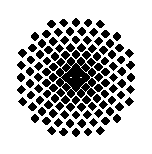
\includegraphics[width=20mm]{university-logo}
	\hspace{6mm}
	\ifthenelse{\equal{\doclang}{german}}{
		\begin{minipage}[b]{.6\textwidth}
		{\Large Universit\"at Stuttgart } \\
		Institut f\"ur Signalverarbeitung und Systemtheorie\\
		Professor Dr.-Ing. B. Yang \vspace{0pt}
		\end{minipage}
	}{
		\begin{minipage}[b]{.6\textwidth}
		{\Large University of Stuttgart } \\
		Institute for Signal Processing and System Theory\\
		Professor Dr.-Ing. B. Yang \vspace{0pt}
		\end{minipage}
	}
	\hspace{1mm}
	
\includegraphics[width=28mm]{isslogocolor}
}
\subject{\worksubject\vspace*{-5mm}} % Art und Nummer der Arbeit
\title{\maintitle}%\\ \Large{\subtitle}}
\subtitle{\translatedtitle}
\author{
\large
  \ifthenelse{\equal{\doclang}{german}}{
  \begin{tabular}{rp{7cm}}
    \Large 
    Autor:      & \Large \student \vspace*{2mm}\\
    Ausgabe:    & \startdate \\
    Abgabe:     & \submission \vspace*{3mm}\\
    Betreuer:   & \tutor \vspace*{2mm}\\
    Stichworte: & \keywords
  \end{tabular}
  }{
  \begin{tabular}{rp{7cm}}
    \Large 
    Author:             & \Large \student \vspace*{2mm}\\
    Date of work begin: & \startdate \\
    Date of submission: & \submission \vspace*{3mm}\\
    Supervisor:         & \tutor \vspace*{2mm}\\
    Keywords:           & \keywords
  \end{tabular}
  }
  \bugfix
}
\date{}
\publishers{\normalsize
  \newpage
  \thispagestyle{empty}
  \begin{minipage}[t]{.9\textwidth}
    \abstract
  \end{minipage}
}

\numberwithin{equation}{chapter} 
\sloppy 

%
%
%
% *****************************************************************
% --------------> put typography definitions here <----------------
% *****************************************************************
% colors
\definecolor{darkblue}{rgb}{0,0,0.4}

% declarations
\newcommand{\matlab}{\textsc{Matlab}\raisebox{1ex}{\tiny{\textregistered}} }
% Integers, natural, real and complex numbers
\newcommand{\Z}{\mathbb{Z}}
\newcommand{\N}{\mathbb{N}}
\newcommand{\R}{\mathbb{R}}
\newcommand{\C}{\mathbb{C}}
% expectation operator
\newcommand{\E}{\operatorname{E}}
% imaginary unit
\newcommand{\im}{\operatorname{j}}
% Euler's number with exponent as parameter, e.g. \e{\im\omega}
\newcommand{\e}[1]{\operatorname{e}^{\,#1}}
% short command for \operatorname{}
\newcommand{\op}[1]{\operatorname{#1}}

\newcolumntype{C}[1]{>{\centering\arraybackslash}m{#1}}
% unknown hyphenation rules
\hyphenation{Im-puls-ant-wort Im-puls-ant-wort-ko-ef-fi-zien-ten
Pro-gramm-aus-schnitt Mi-kro-fon-sig-nal}
% *****************************************************************
\makenomenclature
\nomenclature[V]{$V$}{Vertices of a 3D mesh}
\nomenclature[V]{$v$}{One vertice of a 3D mesh}
\nomenclature[V]{$E$}{Triangles of a 3D mesh}
\nomenclature[V]{$e$}{One triangle of a 3D mesh}
\nomenclature[V]{$\mathbf{t}$}{3D translation vector}
\nomenclature[V]{$\mathbf{R}$}{3D rotation matrix}
\nomenclature[V]{$r_{ij}$}{Elements in 3D rotation matrix}
\nomenclature[V]{$\mathbf{r}$}{Representation of 3D rotation in vector form}
\nomenclature[V]{$\mathbf{T}$}{3D transformation matrix}
\nomenclature[V]{$t_{x,y,z}$}{Translation scalars in three orthogonal directions}
\nomenclature[V]{$\Phi_{x,y,z}$}{Euler angles in three orthogonal directions}
\nomenclature[V]{$O$}{Object set}
\nomenclature[V]{$M$}{Mesh of an object}
\nomenclature[S]{$\mathbb{R}$}{Real number set}
\nomenclature[S]{$\mathbb{SO}(3)$}{3D special orthogonal group}
\nomenclature[S]{$\mathbb{SE}(3)$}{3D special Euclidean group}
\nomenclature[V]{$q$}{Quaternion}
\nomenclature[V]{$\mathbf{q}$}{Quaternion in vector form}
\nomenclature[V]{$q_{w,x,y,z}$}{Quaternion coefficients}
\nomenclature[F]{$f_{GS}$}{Gram-Schmidt-like process}
\nomenclature[F]{$g_{GS}$}{Reverse Gram-Schmidt-like process}
\nomenclature[F]{$N(\cdot)$}{Normalization function}
\nomenclature[F]{$V(D,G)$}{Value function of GAN}
\nomenclature[N]{$D$}{Discriminator of GAN}
\nomenclature[N]{$G$}{Generator of GAN}
\nomenclature[F]{$\mathbb{E}(\cdot)$}{Expectation of a random variable}
\nomenclature[F]{$KL(P\parallel Q)$}{Kullback-Leibler divergence}
\nomenclature[F]{$\odot $}{Element-wise multiplication}
\nomenclature[D]{$\mathcal{N}(\mu,\sigma^{2})$}{Normal distribution with mean $\mu$ and variance $\sigma^{2}$}
\nomenclature[V]{$\epsilon$}{Random noise with normal distribution}
\nomenclature[V]{$\epsilon_{t}$}{Random noise with normal distribution at time step $t$}
\nomenclature[V]{$\epsilon_{\theta}$}{Estimated noise}
\nomenclature[C]{$I$}{Identity matrix}
\nomenclature[C]{$\alpha_{t},\beta_{t}$}{Variance schedule of diffusion models}
\nomenclature[C]{$\bar{\alpha}_{t},\bar{\beta}_{t}$}{Accumulated variance schedule of diffusion models}
\nomenclature[V]{$\mathbf{x}_{t}$}{Data at time step $t$ of diffusion models}
\nomenclature[V]{$\mathbf{\mu}_{\theta}(\mathbf{x}_{t},t)$}{Estimated mean at time step $t$ in tensor form}
\nomenclature[V]{$\mathbf{\Sigma}_{\theta}(\mathbf{x}_{t},t)$}{Estimated variance at time step $t$ in tensor form}
\nomenclature[V]{$\mathbf{\tilde{\mu}}_{t}$}{Trackable mean at time step $t$ in tensor form}
\nomenclature[V]{$\tilde{\beta}_{t}$}{Trackable variance at time step $t$}
\nomenclature[F]{$L$}{Loss function}
\nomenclature[V]{$t$}{Time step variable}
\nomenclature[C]{$T$}{Diffusion steps}
\nomenclature[V]{$y$}{Conditional input of conditional diffusion models}
\nomenclature[V]{$z$}{Latent feature}
\nomenclature[V]{$\mathbf{f}(\mathbf{x},t)$}{Drift term of SDE}
\nomenclature[V]{$g(t)$}{Diffusion coefficient of SDE}
\nomenclature[F]{$\mathbf{w}$}{Brownian motion}
\nomenclature[F]{$D_{F}$}{Fisher divergence}
\nomenclature[V]{$\mathbf{s}_{\theta}$}{Estimated score of SGM}
\nomenclature[D]{$\mathcal{U}(0,T)$}{Uniform distribution between 0 and $T$}
\nomenclature[F]{$\lambda(t)$}{Weighting function of SDE}
\nomenclature[V]{$\mathbf{T}_{t}$}{Transformation at time step $t$}
\nomenclature[V]{$\mathbf{T}_{r}$}{Refined transformation}
\nomenclature[C]{$\eta$}{Hyperparemeter that controls the sampling stochasticity}
\nomenclature[V]{$\tau_{1,...,s}$}{Subset of the complete diffusion steps in DDIM}
\nomenclature[V]{$\mathbf{q}_{i},\mathbf{k}_{i},\mathbf{v}_{i}$}{Query, key and value vectors of the attention mechanism}
\nomenclature[V]{$\mathbf{W}^{q,k,v}$}{Query, key and value matrices of the attention mechanism}
\nomenclature[V]{$\mathbf{W}^{O}$}{Output matrix of the attention mechanism}
\nomenclature[C]{$d_{k}$}{Dimension of the key vector}
\nomenclature[V]{$\mathbf{y}_{i}$}{Output vector of the scaled dot-product attention}
\nomenclature[V]{$\mathbf{h}_{i}$}{Output matrix of a single head attention}
\nomenclature[V]{$\alpha_{1,2},\beta_{1,2},\gamma_{1,2}$}{Learnable parameters of AdaLN}
\nomenclature[F]{$H(a,b)$}{Cross-entropy function}
\nomenclature[N]{$g_{\theta_{t}}$}{Teacher network in knowledge distillation}
\nomenclature[N]{$g_{\theta_{s}}$}{Teacher network in knowledge distillation}
\nomenclature[V]{$\theta_{s}$}{Student parameters in knowledge distillation}
\nomenclature[V]{$S$}{Reference point cloud in completion task}
\nomenclature[V]{$\hat{S}$}{Reconstruct point cloud in completion task}
\nomenclature[C]{$d$}{Feature dimension}
\nomenclature[C]{$B,b$}{Batch size}
\nomenclature[V]{$f_{2D}$}{2D global feature}
\nomenclature[V]{$f_{3D}$}{3D global feature}
\nomenclature[V]{$e_{p}$}{Position embedding}
\nomenclature[V]{$e_{t}$}{Time embedding}
\nomenclature[C]{$n_{nb}$}{Number of neighbors}
\nomenclature[V]{$\mathcal{T}_{B}$}{Subset of the whole timesteps with the batch size $B$}
\nomenclature[V]{$\hat{\mathbf{P}},\bar{\mathbf{P}}$}{Estimated pose and ground truth pose}
\nomenclature[V]{$\hat{S},\bar{S},S_{I}$}{Estimated, ground truth and test image distance map}
\nomenclature[C]{$\tau$}{Misalignment tolerence of VSD}
\nomenclature[V]{$e_{metric}$}{Error of the evaluation metric}
\nomenclature[C]{$\theta_{e}$}{Threshold of the recall rate calculation}
\nomenclature[D]{$h(\mathbf{T}\vert y)$}{Distribution of the transformation hypotheses conditioned with the input}
\nomenclature[D]{$q(\mathbf{x}_{t}\vert\mathbf{x}_{t-1})$}{Forward diffusion process between each time step}
\nomenclature[D]{$q(\mathbf{x}_{t-1}\vert\mathbf{x}_{t})$}{Reverse diffusion process between each time step}
\nomenclature[D]{$p_{\theta}(\mathbf{x}_{t-1}\vert\mathbf{x}_{t})$}{Estimated reverse diffusion process between each time step}
\renewcommand{\nomname}{List of Symbols}
\setlength{\nomlabelwidth}{2.5cm}
\renewcommand\nomgroup[1]{%
  \item[\bfseries
  \ifstrequal{#1}{C}{Constants}{%
  \ifstrequal{#1}{F}{Functions}{%
  \ifstrequal{#1}{V}{Variables}{%
  \ifstrequal{#1}{N}{Networks}{%
  \ifstrequal{#1}{D}{Distributions}{%
  \ifstrequal{#1}{S}{Fields}{}}}}}}%
]}
% *****************************************************************
\renewcommand*{\glsdohyperlink}[2]{{\hypersetup{linkcolor=black}\hyperlink{#1}{#2}}}
\glsenablehyper
\makeglossaries
\newacronym{6dof}{6 DoF}{six degrees of freedom}
\newacronym{3d}{3D}{three-dimensional}
\newacronym{2d}{2D}{two-dimensional}
\newacronym{1d}{1D}{one-dimensional}
\newacronym{rgb}{RGB}{red, green, blue}
\newacronym{rgbd}{RGB-D}{red, green, blue, depth}
\newacronym{ddpm}{DDPM}{Denoising Diffusion Probabilistic Models}
\newacronym{ddim}{DDIM}{Denoising Diffusion Implicit Models}
\newacronym{d3pm}{D3PM}{Discrete Denoising Diffusion Probabilistic Models}
\newacronym{cad}{CAD}{Computer-Aided Design}
\newacronym{mrp}{MRP}{Modified Rodrigues Parameters}
\newacronym{icp}{ICP}{Iterative Closest Point}
\newacronym{gicp}{GICP}{Generalized Iterative Closest Point}
\newacronym{nicp}{NICP}{Normal Iterative Closest Point}
\newacronym{pnp}{P$n$P}{Perspective-$n$-Point}
\newacronym{ar}{AR$^*$}{Augmented Reality}
\newacronym{avre}{AR}{Average Recall}
\newacronym{lm}{LM}{LINEMOD}
\newacronym{lmo}{LMO}{LINEMOD-Occlusion}
\newacronym{gan}{GAN}{Generative Adversarial Network}
\newacronym{vae}{VAE}{Variational Autoencoder}
\newacronym{vqvae}{VQ-VAE}{Vector Quantized Variational Autoencoder}
\newacronym{cv}{CV}{Computer Vision}
\newacronym{sr3}{SR3}{Super-Resolution via Repeated Refinement}
\newacronym{cdm}{CDM}{Cascaded Diffusion Models}
\newacronym{idm}{IDM}{Implicit Diffusion Models}
\newacronym{nerf}{NeRF}{Neural Radiance Fields}
\newacronym{sift}{SIFT}{Scale-Invariant Feature Transform}
\newacronym{surf}{SURF}{Speeded Up Robust Features}
\newacronym{orb}{ORB}{Oriented FAST and Rotated BRIEF}
\newacronym{ransac}{RANSAC}{Random Sample Consensus}
\newacronym{cnn}{CNN}{Convolutional Neural Network}
\newacronym{mlp}{MLP}{Multilayer Perceptron}
\newacronym{rcnn}{R-CNN}{Region-based Convolutional Neural Network}
\newacronym{sgm}{SGM}{Score-based Generative Model}
\newacronym{sde}{SDE}{Stochastic Differential Equation}
\newacronym{pdf}{PDF}{Probability Density Function}
\newacronym{ode}{ODE}{Ordinary Differential Equation}
\newacronym{nlp}{NLP}{Natural Language Processing}
\newacronym{cas}{CAS}{Consistent Annealed Sampling}
\newacronym{ald}{ALD}{Annealed Langevin Dynamics}
\newacronym{ddss}{DDSS}{Differentiable Diffusion Sampler Search}
\newacronym{elbo}{ELBO}{Evidence Lower Bound}
\newacronym{vdm}{VDM}{Variational Diffusion Models}
\newacronym{csm}{CSM}{Concrete Score Matching}
\newacronym{rdm}{RDM}{Riemannian Diffusion Model}
\newacronym{rsgm}{RSGM}{Riemmanian Score-based Generative Model}
\newacronym{lsgm}{LSGM}{Latent Score-based Generative Model}
\newacronym{ldm}{LDM}{Latent Diffusion Model}
\newacronym{vit}{ViT}{Vision Transformer}
\newacronym{ln}{LN}{Layer Normalization}
\newacronym{adaln}{AdaLN}{Adaptive Layer Normalization}
\newacronym{ema}{EMA}{Exponential Moving Average}
\newacronym{sg}{SG}{Stop-Gradient}
\newacronym{bop}{BOP}{Benchmark for 6D Object Pose Estimation}
\newacronym{pbr}{PBR}{Physically Based Rendering}
\newacronym{knn}{$k$-NN}{$k$-Nearest Neighbors}
\newacronym{cd}{CD}{Chamfer Distance}
\newacronym{mse}{MSE}{Mean Squared Error}
\newacronym{vsd}{VSD}{Visible Surface Discrepancy}
\newacronym{mssd}{MSSD}{Maximum Symmetry-Aware Surface Distance}
\newacronym{mspd}{MSPD}{Maximum Symmetry-Aware Projection Distance}
\newacronym{add}{ADD}{Average Distance}
\newacronym{adds}{ADD-S}{Average Distance for Symmetrical Objects}
\newacronym{ca}{CA}{Cosine Annealing}
\newacronym{lr}{lr}{learning rate}
\newacronym{adam}{Adam}{Adaptive Moment Estimation}
\newacronym{roi}{RoI}{Region of Interest}

\glsaddall
\newglossarystyle{custom_acronyms}
{

    \setglossarystyle{long3col}%
    \renewcommand*{\glossaryheader}{}%
    \renewcommand{\glossentry}[2]{%
        \textbf{\glsentryitem{##1}\glstarget{##1}{\glossentryname{##1}}}
        & \glossentrydesc{##1}
        & ##2
        \tabularnewline}%
}
% *****************************************************************
\begin{document}

% title and table of contents
\pagenumbering{alph}
\maketitle
\cleardoublepage
\pagenumbering{roman} % roman numbering for table of contents
\tableofcontents
\cleardoublepage
\setcounter{page}{1}
\pagenumbering{arabic} % arabic numbering for rest of document

% *****************************************************************
% -------------------> start writing here <------------------------



\setlength\LTleft{-5pt}
\printglossary[type=\acronymtype,title=List of Acronyms,nonumberlist,style=custom_acronyms]

\printnomenclature

\chapter{Introduction}
\section{Motivation}
In recent years, the field of \gls{cv} has undergone a significant transformation, fueled by the rapid advancement and integration of cutting-edge technologies such as deep learning and the utilization of \gls{3d} data. This transformation has substantially enhanced machines' capabilities to comprehend and interact with the physical world. Within the realm of computer vision, \gls{6dof} pose estimation, tasked with determining the position and orientation of objects in \gls{3d} space, has garnered considerable attention due to its pivotal role in diverse applications, including augmented reality, robotics, automation, autonomous driving, object manipulation, and quality control.

\gls{6dof} pose estimation necessitates the integration of techniques from various fields. Learning-based methods are employed to extract features from input data and estimate poses, while non-learning-based algorithms process and refine these estimations. To accommodate diverse data inputs and enhance accuracy and reliability, the task involves processing data from both \gls{2d} and \gls{3d} domains. Scaling to multi-object or multi-view scenarios, commonplace in robotics and autonomous driving, and considering time-series data introduce additional challenges and opportunities. Pose estimation can extend beyond its core function to object tracking in videos or even predicting future object poses. The complexity of these tasks intensifies the challenge of pose estimation in real-world applications, injecting vitality into ongoing research in this field.

Diffusion models, initially introduced by Sohl-Dickstein et al. 2015 \cite{sohldickstein2015deep} and recently refined by Ho et al. 2020 \cite{ho2020denoising}, belong to a class of generative models renowned for their capacity to generate high-quality data from random noise. Demonstrating notable success in various image synthesis tasks, diffusion models have outperformed previous methods, extending their influence beyond \gls{cv} to fields such as natural language processing, temporal data modeling, and multi-model learning. Despite this success, the integration of diffusion models into \gls{6dof} pose estimation is at an early stage, with limited existing works. The untapped potential of these models in the realm of \gls{6dof} pose estimation underscores a promising avenue for exploration and advancement in the field.

The widespread use of \glsunset{rgbd}\gls{rgbd} images in computer vision tasks stems from the increased prevalence of \gls{rgbd} sensors and the invaluable depth information they provide. Research consistently indicates that leveraging depth information alongside \glsunset{rgb}\gls{rgb} data leads to improvements in network performance, surpassing the capabilities of methods reliant solely on \gls{rgb} data. Given this, it is of great significance to evaluate the effectiveness of diffusion models when applied to \gls{rgbd} data within the context of our pose estimation task. This evaluation will shed light on the model's capability to harness the additional depth information for enhanced pose estimation accuracy and robustness.
\section{Aims and Objectives}
This thesis endeavors to explore the feasibility of integrating diffusion models into the pose estimation task, harnessing the advantages inherent in diffusion models within the \gls{2d} domain and extending their utility to the \gls{3d} domain. These advantages encompass the capability of handling large-scale data and the diversity of the generated data. To this end, we first review the related works about the \gls{6dof} pose estimation and diffusion models. Then design the diffusion network architecture with the single \gls{rgbd} image as input, which contains the diffusion backbone, \gls{2d} feature extractor and \gls{3d} feature extractor. Finally, we evaluate the performance of the diffusion models on the \gls{6dof} pose estimation task and compare it with the preceding methods characterized by varying architectural configurations.
\section{Structure of the Thesis}
The thesis is organized into seven chapters and the structure of the thesis is as follows:
\begin{description}
  \item[Chapter 2 - Background] This chapter gives an overview of the \gls{6dof} pose estimation and diffusion models. The \gls{6dof} pose estimation is introduced with the definition, representation of the pose and typical applications. The challenges of the pose estimation task are also discussed. The diffusion models are introduced with an overview of other generative models and the basic theory behind them together with the applications.
  \item[Chapter 3 - Related Works] In this chapter, some previous works are reviewed which are related to the \gls{6dof} pose estimation and diffusion models. Different architectures of the pose estimation models are hierarchically introduced and discussed.
  \item[Chapter 4 - Methodology] The proposed method and models are introduced in this chapter. The structure of the pose diffusion architecture is presented together with each module and algorithm of the model in detail.
  \item[Chapter 5 - Experiments] The experiments are conducted in this chapter. The datasets and evaluation metrics are introduced first. We describe the setup of the training and evaluation for each model in this work. Then the qualitative and quantitative results of the experiments, the comparison with other methods as well as the ablation study are presented.
  \item[Chapter 6 - Discussion] The results of the experiments are discussed here. The advantages and disadvantages of the proposed method are analyzed and the possible improvements are also discussed.
  \item[Chapter 7 - Conclusion ] Finally, we summarize the thesis and the contribution from this work and give an outlook of future work.
\end{description} 

\chapter{Background}
\section{6 DoF Pose Estimation}
\subsection{Definition}
The term "Six Degrees of Freedom (6DoF) pose" pertains to the six fundamental ways a rigid body can move within three-dimensional space. Specifically, it encompasses the freedom of movement in three orthogonal directions, referred to as translations, as well as the ability to rotate about three orthogonal axes, termed rotations. This concept holds significant relevance, particularly in industrial and automotive domains, where it is instrumental in measuring and analyzing the spatial properties of objects. The comprehensive understanding of an object's movement and orientation provided by the 6DoF pose is crucial for various applications within these fields.

In domain of computer vision and robotics, \gls{6dof} pose estimation is a fundamental task that aims to estimate the \gls{3d} translation $\mathbf{t}=(t_{x} ,t_{y} ,t_{z} )$ and rotation $\mathbf{R}=(\Phi_{x} ,\Phi_{y} ,\Phi_{z} )$ of an object related to a canonical coordinate system using the sensor input, such as \gls{rgb} or \gls{rgbd} data.The object $M$ is typically a known \gls{3d} \gls{cad} model, consisting of a set of vertices $V=\{v_1,...,v_N\}$, with $v_i\in \mathbb{R}^3$ and $V\in \mathbb{R}^{3 \times N}$ and triangles $E=\{e_1,...,e_M\}$, with $e_i\in \mathbb{R}^3$ and $E\in \mathbb{R}^{3\times M}$ connecting the vertices. Furthermore, if the query image is a multi-object scenario with N objects $O=\{M_1,...,M_N\}$, we need to detect and estimate the pose of each object $M_i$ in the image \cite{Fabian_2021}. The following figure \ref{img:6d} shows a general structure of the learning-based \gls{6dof} pose estimation.

\begin{figure}[h]
	\centering
	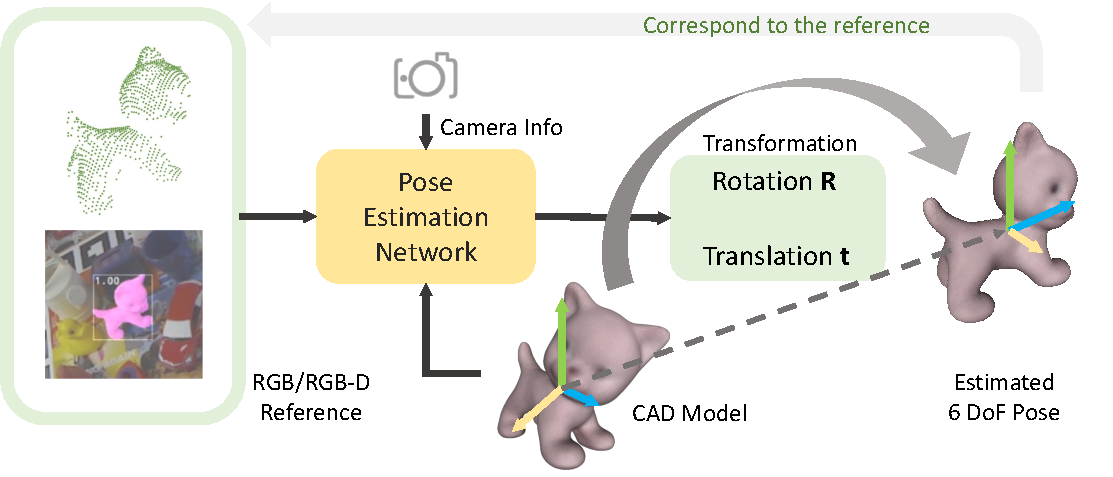
\includegraphics[width=1.\textwidth]{img/6d.pdf}
	\caption{Overview of the general proposal towards 6 DoF pose estimation.}
	\label{img:6d}
\end{figure}

\subsection{Representing 6 DoF Pose}\label{sec:representation}
\gls{6dof} pose can be treated seperately as \gls{3d} translation and \gls{3d} rotation. The \gls{3d} translation is simply represented by 3 scalars along the X, Y, and Z axis of the canonical coordinate system. 
We can use either the deep learning methods to estimate the depth and the corresponding \gls{2d} projection from \gls{rgb} images or even get the depth information fused from \gls{rgbd} data \cite{DBLP:journals/corr/abs-1711-00199}. After that, the object can be shifted back to the camera coordinate system by adding a translation vector to the object vertices $V$:
\begin{align}
  V^{'} = V + \mathbf{t}
\end{align}
where $V^{'}$ represents the shifted object vertices. Similarly, the \gls{3d} rotation can be represented by 3 rotation matrices around the X, Y and Z axes. The final transformation of rotation can be achieved by multiplying the rotation matrices $\mathbf{R}_{i}$ defined by Euler angles $\Phi_{i}$ with $i\in \{X,Y,Z\}$. Rotation around X axis is defined as:
\begin{align}
  V^{'} = \mathbf{R}_{X}(\Phi_{x})V = \begin{bmatrix}
    1 & 0 & 0 \\
    0 & cos(\Phi_{x}) & -sin(\Phi_{x}) \\
    0 & sin(\Phi_{x}) & cos(\Phi_{x})
  \end{bmatrix}V
\end{align}
Rotation matrix $\mathbf{R}_{Y}$ and $\mathbf{R}_{Z}$ can be defined repectively with:
\begin{align}
  \mathbf{R}_{Y}(\Phi_{y}) = \begin{bmatrix}
    cos(\Phi_{y}) & 0 & sin(\Phi_{y}) \\
    0 & 1 & 0 \\
    -sin(\Phi_{y}) & 0 & cos(\Phi_{y})
  \end{bmatrix}
\end{align}
\begin{align}
  \mathbf{R}_{Z}(\Phi_{z}) = \begin{bmatrix}
    cos(\Phi_{z}) & -sin(\Phi_{z}) & 0 \\
    sin(\Phi_{z}) & cos(\Phi_{z}) & 0 \\
    0 & 0 & 1
  \end{bmatrix}
\end{align}
The rotation matrix $\mathbf{R}$ can be obtained by multiplying the three rotation matrices $\mathbf{R}_{X}$, $\mathbf{R}_{Y}$ and $\mathbf{R}_{Z}$ together, but changing the order of the multiplication will result in different rotation matrix. The common order is defined as $Z-Y-X$ order, which means the rotation around the X axis is performed first, then the Y axis and finally the Z axis. All possible rotations in \gls{3d} Euclidean space establish a natural manifold known as special orthogonal group $\mathbb{S} \mathbb{O} (3)$ \cite{hashim2019special}.

Togather with the translation vector $\mathbf{t}$, the \gls{6dof} pose can be represented by a 4x4 transformation matrix $\mathbf{T}$ as:
\begin{align}
  \mathbf{T} = \begin{bmatrix}
    \mathbf{R} & \mathbf{t} \\
    0 & 1
  \end{bmatrix}
  = \begin{bmatrix}
    r_{11} & r_{12} & r_{13} & t_{1} \\
    r_{21} & r_{22} & r_{23} & t_{2} \\
    r_{31} & r_{32} & r_{33} & t_{3} \\
    0 & 0 & 0 & 1
  \end{bmatrix}
  \in \mathbb{S} \mathbb{E} (3)
\end{align}
The partitioned transformation matrix with 3x3 rotation matrix $\mathbf{R}$ and a column vector $\mathbf{t}$ that represents the translation is also called the homogeneous representation of a transformation. All possible transformation matrices of this form generate the special Euclidean group $\mathbb{S} \mathbb{E} (3)$:
\begin{align}
  \mathbb{S} \mathbb{E} (3) = \{\mathbf{T} = \begin{bmatrix}
    \mathbf{R} & \mathbf{t} \\
    0 & 1
  \end{bmatrix}\in \mathbb{R}^{4 \times 4}| \mathbf{R} \in \mathbb{S} \mathbb{O} (3), \mathbf{t} \in \mathbb{R}^{3} \}
\end{align}
Normally, we use the shift in 3 orthogonal directions in the cartesian coordinate system to represent the translation. However, there are some different ways to represent the rotation.

One simple method to represent the rotation is to use the Euler angles $\phi$, $\theta$ and $\psi$ which are also marked as roll angle (around X axis), pitch angle (around Y axis) and yaw angle (around Z axis) respectively. The main drawback of this representation is the gimbal lock problem, which means the rotation around two axes will cause the rotation around the third axis to be the same as the rotation around the first axis.

An alternative representation of \gls{6dof} pose is a 4-dimensional vector that consists of translation and rotation quaternion which has a compacter form:
\begin{align}
  \mathbf{r} = (q_{w}, q_{x}, q_{y}, q_{z})^{T}
\end{align}
Where the quaternion $q$ is defined as:
\begin{align}
  q = q_{w} + q_{x}i + q_{y}j + q_{z}k \quad \textrm{with} \quad i^{2} = j^{2} = k^{2} = ijk = -1
\end{align}
Normally, regressing the rotation matrix directly is not a common choice since the same rotation can be achieved via different combinations of Euler angles. And the unit quaternion form is in many cases preferred because it can ensure the uniqueness by restricting the quaternion on the upper hemisphere of $q_{w}=0$ plane and can also guarantee a gimbal-lock free rotation in $\mathbb{S} \mathbb{O} (3)$ \cite{9231126}. 

Another representation that can be considered is called \glspl{mrp} which is a 3-dimensional vector $\mathbf{r} = (r_{1}, r_{2}, r_{3})^{T}$. They are triplets in $\mathbb{R}^{3} $, bijectively and rationally mapped to quaternions through stereographic projection \cite{rodrigues}. The \gls{mrp} vector $\mathbf{r}$ is defined as:
\begin{align}
  \mathbf{r} = \frac{\mathbf{q}}{1+q_{w}} = \frac{1}{1+q_{w}}(q_{x}, q_{y}, q_{z})^{T}
\end{align}
where $\mathbf{q}$ is the quaternion representation of the rotation. The \gls{mrp} vector $\mathbf{r}$ is also a unit vector, the advantage of using \gls{mrp} is that a random assignment of the vecter within the unit sphere will always result in a valid rotation. That property makes this representation more robust in the forward and reverse process of the diffusion pipeline.

Zhou et al. 2019 \cite{Zhou_2019_CVPR} proposed a novel representation of rotation called 6D continuous rotation representation. The mapping from the rotation matrix to the 6D representation with generally $n$ dimensional rotation is defined as:
\begin{align}
  g_{GS}\left( \
    \begin{bmatrix}
      | & & | \\
      a_{1}  & \cdots & a_{n} \\
      | & & |
    \end{bmatrix} \
  \right) = 
  \begin{bmatrix}
    | & & | \\
    a_{1}  & \cdots & a_{n-1} \\
    | & & |
  \end{bmatrix}
\end{align}
The mapping from $\mathbb{S} \mathbb{O} (3)$ to the 6D representation can be simplified as:
\begin{align}\label{eq:ortho6d}
  g_{GS}\left( \
    \begin{bmatrix}
      | & | & | \\
      a_{1}  & a_{2} & a_{3} \\
      | & | & |
    \end{bmatrix} \
  \right) = 
  \begin{bmatrix}
    | & | \\
    a_{1} & a_{2} \\
    | & |
  \end{bmatrix}
\end{align}
The reverse mapping follows the Gram-Schmidt-like process:
\begin{gather}
  f_{GS}\left( \ 
    \begin{bmatrix}
      | & | \\
      a_{1}  & a_{2}  \\
      | & | 
    \end{bmatrix} \
  \right) = 
  \begin{bmatrix}
    | & | & |\\
    b_{1} & b_{2} & b_{3}\\
    | & | & |
  \end{bmatrix} \\
  b_{i} = \left[\left\{
    \begin{array}{lr}
    N(a_{1}) & \text{if} \ i=1\\
    N(a_{2}-(b_{1}\cdot a_{2})b_{1}) & \text{if} \ i=2\\
    b_{1}\times b_{2}& \text{if} \ i=3
    \end{array} 
  \right.
  \right] ^{T}
\end{gather}
Here $N(\cdot)$ is the normalization function. It was proved by the sanity tests introduced in the paper that this kind of representation is an efficient way for training in deep neural networks, compared with quaternions and Euler angles that are not continuous and have singularities.
\subsection{Applications}
\gls{6dof} pose estimation is a central technology that can be the critical part of many computer vision applications such as augmented \gls{ar}, robotics, \gls{3d} scene understanding and autonomous driving. In this section, we will introduce some typical applications of \gls{6dof} pose estimation.

\subsubsection{Augmented Reality}
\gls{ar} applications use \gls{6dof} pose estimation to accurately place the virtual objects in the real world. Precise estimation and quick inference of the pose guarantee an immersive and interactive experience 
which is the direction of the development of \gls{ar} applications \cite{9836663}. Furthermore, \gls{6dof} pose estimation can also be utilized to track real-world objects, enabling more natural interactions.

\subsubsection{Robotics}
\gls{6dof} pose estimation helps robots understand the scene so that the grasping and manipulation of objects can be achieved. In the field of medical robotics, it can be used to track the surgical instrument or a patient's body part \cite{cao20236impose}. In manufacturing, robots use the estimated pose to identify, sort and assemble the objects in the field like automatic logistic sorting and manufacturing lines.

\subsubsection{3D Scene Understanding}
In order to register the \gls{3d} objects into the scene or reconstruct the \gls{3d} environment from \gls{2d} images or \gls{3d} point clouds, \gls{6dof} pose estimation is required. The alignment of the \gls{3d} objects or \gls{3d} scenes is realized by estimating the rigid transformation using methods like correspondence matching \cite{qin2022geometric} or direct transformation estimation \cite{fu2021robust} follows the ideas of \gls{icp} \cite{Besl1992AMF}.

\subsubsection{Autonomous Driving}
Autonomous driving is also a cross-domain topic that requires many different technologies to work together. A well-estimated pose of the vehicle inside the scene is the basis of many other subtasks of autonomous driving such as collision avoidance, trajectory planning and so on. Subtle errors in the pose estimation may lead to fatal consequences \cite{auto} because the vehicle moves normally at high speed and the heading direction causes a large deviation in a long distance considering also the reaction time of the vehicle.
\subsection{Challenges}
\gls{6dof} pose is widely used in many applications and has become a popular research topic of computer vision in recent years. However, solving this problem is not trivial and even challenging in many cases.

The first constraint would be the auto-occlusion or symmetries of the object since the object cannot be clearly and unequivocally observed from all angles \cite{maru2022}. The auto-occlusion means that the object itself is partially occluded by other parts of the object such as \gls{lmo} dataset  \cite{dataV4MUMX2020}. This is common in many real-world objects such as tables or chairs. The symmetry of the object means that the object has the same appearance from different angles, which will cause ambiguity in the estimation such as the T-LESS dataset \cite{hodan2017tless}. Imagining an image of a mug with the handle hidden behind it, it is hard to tell the orientation of the mug without the handle.

Textureless object is also a challenge for \gls{6dof} pose estimation since many methods rely not only on the geometry of the object but also on the texture. It is hard for \gls{rgb}-only methods \cite{kendall2016posenet} or keypoint-based method \cite{pavlakos20176dof} to extract enough local features if the object is completely textureless.

Another difficulty is the domain gap between the training and testing data. Normally, the training data consists of synthetic \gls{cad} models and images which are clean and annotated with the ground truth pose to have precise supervision. But lacking the information of the real world, for example, lighting and occlusion, the model trained on the synthetic data cannot generalize well to the real world data. Some dataset provides real-world data or \gls{3d} rendered images which can reduce the domain gap to some degree \cite{hodan2019photorealistic}, but the noise and invalid training samples still confuse the model.

If facing the multi-object scenario, which is common in applications like robotics and autonomous driving, the unknown number and type of objects will increase the difficulty of pose estimation for each object in the scene.

\section{Diffusion Models}
\subsection{Generative Models}
One of the most fascinating and distinctive features of the human brain is the ability to create or imagine objects that do not immediately exist in reality. Humans can spontaneously learn the underlying properties of the world and generate hypotheses about the future. This procedure is similar to supervised learning and reinforcement learning with little amount of labeled data but generalizes very well to many unseen scenarios and has a high level of robustness \cite{lamb2021brief}.

In order to achieve a similar ability of the generative process from the human brain, many generative models have been proposed in recent years, to not synthesize the unseen data but to recover or modify the seen data with given constraints. Some of the most popular generative models are introduced below.

\subsubsection{Generative Adversarial Networks}
\glspl{gan} \cite{goodfellow2014generative} is a smart idea to train a generative model by playing a min-max game between two neural networks. The generator $G$ is trained to generate data that is indistinguishable from the real data, while the discriminator $D$ is trained to distinguish the real data from the fake data generated by $G$. The training process can be formulated as the value function $V(D,G)$, and for the classification objective using cross-entropy loss, the optimization problem can be written as:
\begin{align}
  \min_{G} \max_{D} V(D,G) = \mathbb{E}_{x\sim p_{data}(x)}[\log D(x)] + \mathbb{E}_{z\sim p_{z}(z)}[\log(1-D(G(z)))]
\end{align}
The generator is optimized to maximize the probability that the discriminator will classify the generated data as real, which explains the word "adversarial" in the name of \gls{gan}.

\glspl{gan} have shown great success in many applications such as generating high-resolution images that are difficult to distinguish from the real ones and the ability to learn the complicated distributions. However, the main challenge of \glspl{gan} is the instability of the training process, which increases the difficulty of training and tuning the model. It will sometimes suffer from the mode collapse problem, where the generator only learns to generate a subset of the data distribution \cite{borji2018pros}.

Some work has been done to solve these problems. For example, Wasserstein \glspl{gan} \cite{arjovsky2017wasserstein} uses a different loss function to stabilize the training process and avoid the mode collapse. Spectral Normalization \cite{miyato2018spectral} is another method to stabilize the training process by constraining the Lipschitz constant of the discriminator.
\subsubsection{Variational Autoencoders}
\glspl{vae} \cite{kingma2022autoencoding} is another popular generative model that is based on the encoder-decoder architecture. It allows the model to learn the latent representation of the input data and generate new data from the latent space. The encoder $E$ is trained to map the input data $x$ to the latent space $z$ with a distribution $q(z|x)$, while the decoder $D$ is trained to reconstruct the input data from the latent space $z$ with a distribution $p(x|z)$. The training process can be formulated as:
\begin{align}
  \min_{E,D} \mathbb{E}_{x\sim p_{data}(x)}[\mathbb{E}_{z\sim q(z|x)}[\log p(x|z)]] - KL(q(z|x)||p(z))
\end{align}
The first term is the reconstruction loss, which is the negative log-likelihood of the input data $x$ given the latent representation $z$. The second term is the regularization term, which is the Kullback-Leibler divergence between the latent distribution $q(z|x)$ and the prior distribution $p(z)$. With the regularisation term, we prevent the model from encoding the input data far apart in the latent space, which will cause the model to generate unrealistic data.

The reparameterization trick \cite{kingma2015variational} is introduced afterward to make the stochastic part of the loss function which is the latent representation $z$ differentiable so that the model can be trained with backpropagation. The latent representation $z$ is sampled from a distribution $q(z|x)$, which is normally a Gaussian distribution. The trick constructs the random variable $z$ into the following expression where $\epsilon$ is a random variable sampled from a standard Gaussian distribution.
\begin{align}
  z \in \mathcal{N} (\mu, \sigma^{2}) \longrightarrow z = \mu + \sigma \odot \epsilon, \quad \epsilon \sim \mathcal{N} (0, 1)
\end{align}
\glspl{vae} allow us to easily sample the latent representation $z$ from the prior distribution $p(z)$ and generate novel data from the decoder $D$. It can also be used to make data compression and denoising, which is the main application of autoencoders. Since the flexibility and the robustness of \glspl{vae}, It is widely used in many applications such as image manipulation, text generation and speech synthesis.
\subsubsection{Normalizing Flows}
Normalizing flows \cite{rezende2016variational} are a family of generative models with tractable marginal likelihood which can not be achieved with \glspl{vae}. A normalizing flow is a transformation of a simple distribution into a more complex distribution by a series of invertible and differentiable mappings. By repeating the rule of transformation, the initial probability density "flows" through the sequence of invertible mappings and becomes a valid distribution.

The basic rule for the transformation of densities considers an invertible, smooth mapping $f: \mathbb{R}^{D} \rightarrow \mathbb{R}^{D}$, with inverse $f^{-1} = g$. Transforming a random variable $z$ with distribution $q(z)$ through $f$ results in a random variable $z^{'}  = f(z)$ has a distribution:
\begin{align}
  q(z^{'}) = q(z) \left| \det \frac{\partial f^{-1}}{\partial z^{'}} \right| = q(z) \left| \det \frac{\partial f}{\partial z} \right|^{-1}
\end{align}
The last term is the Jacobian determinant of the transformation $f$, which is the determinant of the matrix of partial derivatives of $f$ with respect to $z$. Given a chain of invertible mappings $f_{1},...,f_{K}$, the transformation of the random variable $z$ through the sequence of mappings and the density $q_{K}(z)$ can be written as:
\begin{gather}
  z_{K} = f_{K} \cdot ... f_{2} \cdot f_{1}(z_{0})\\
  lnq_{K}(z_{K}) = lnq_{0}(z_{0}) - \sum_{k=1}^{K} ln \left| \det \frac{\partial f_{k}}{\partial z_{k-1}} \right|
\end{gather}
The path of the transformation can be seen as a flow of the probability density from the initial distribution $q_{0}(z_{0})$ to the final distribution $q_{K}(z_{K})$. If the length of the normalizing flow tends to infinity, the model becomes an infinitesimal flow which is described by a differential equation.

Normalizing flows provides a flexible framework for modeling complex distributions, which is difficult to achieve with previous generative models. However, the samples that are generated through flow-based models are not as realistic as the samples from \glspl{gan} or \glspl{vae}, and the data will be projected into also high dimensional space, which is hard to interpret.

\subsubsection{Diffusion Models}
Diffusion models are a new class of state-of-the-art generative models that can synthesize high-quality images in recent years. The representative one, which is the \gls{ddpm} was initialized by Sohl-Dickstein et al 2015 \cite{sohldickstein2015deep} and proposed recently by Ho. et al 2020 \cite{ho2020denoising}. 

A diffusion probabilistic model (diffusion model), inspired by the nonequilibrium thermodynamics, is a parameterized Markov chain trained using variational inference to produce samples from a given target distribution after finite steps. The basic idea behind diffusion models is trivial. Given an input data $x_{0}$, we first gradually add Gaussian noise to it and finally get a sequence of noised data $x_{1},...,x_{T}$, which we call it forward process. Afterward, a neural network is trained to recover the original data by estimating the noise and reversing the forward process, which we call it sampling process or reverse process.

Figure \ref{img:gen} shows an overview of four different types of generative models that we mentioned in this section. Unlike \gls{vae} and the flow-based model, the diffusion model is based on the Markov chain and the latent variable has high dimensionality which has the same size as the input data. We recover the original data by estimating the noise and reversing the forward process iteratively, which ensures the high quality of the generated data.

The great success of some architecture using the diffusion model such as GLIDE \cite{nichol2022glide} and DALLE-2/3 \cite{ramesh2022hierarchical} has shown the potential of the diffusion model in the field of generative models. The advantage of the diffusion model is that it is large-scale, flexible and offers high-quality samples. With the tradeoff of the relatively longer training time and inference time because of its 2-phases architecture, it can synthesize the highest-quality images than other generative models. This potential motivates us to apply the diffusion model also to \gls{3d} domain and the related tasks.

\begin{figure}[h]
	\centering
	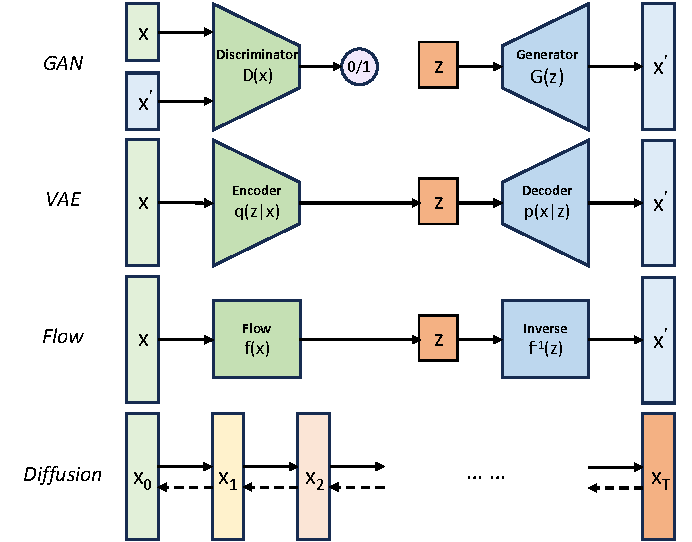
\includegraphics[width=0.9\textwidth]{img/gen.pdf}
	\caption{Overwiew of different types of generative models.}
	\label{img:gen}
\end{figure}

\subsection{Theory and Fundamentals}\label{sec:theory}
In this section, we will introduce the details of the diffusion model, the mathematical background in the forward process and the sampling process, and the conditional diffusion model. The extended version of the classic \gls{ddpm} will also be briefly introduced.

\subsubsection{Forward Process}
Given an input data $\mathbf{x}_{0}$ from the target data distribution $q(\mathbf{x})$, we first define a forward process that gradually adds Gaussian noise to $\mathbf{x}_{0}$ with variance $\beta_{t}\in (0, 1)$ at each step $t$ and finally get a sequence of noised data $\mathbf{x}_{1},...,\mathbf{x}_{T}$. At each step $t$, we have the new data $\mathbf{x}_{t}$ with the conditional distribution $q(\mathbf{x}_{t}|\mathbf{x}_{t-1})$ defined as:
\begin{align}
  q(\mathbf{x}_{t}|\mathbf{x}_{t-1}) = \mathcal{N}(\mathbf{x}_{t}; \sqrt{1-\beta_{t}}\mathbf{x}_{t-1}, \beta_{t}\mathbf{I})
\end{align}
where $q(\mathbf{x}_{t}|\mathbf{x}_{t-1})$ is a normal distribution with mean $\sqrt{1-\beta_{t}}\mathbf{x}_{t-1}$ and variance $\beta_{t}\mathbf{I}$. Thus, we can derive the posterior distribution from the input data $\mathbf{x}_{0}$ to $\mathbf{x}_{T}$ in a tractable way:
\begin{align}
  q(\mathbf{x}_{1:T}|\mathbf{x}_{0}) = \prod_{t=1}^{T}q(\mathbf{x}_{t}|\mathbf{x}_{t-1})
\end{align}

Our goal is to track the noised data at an arbitrary step $t$ with a closed-form posterior distribution $q(\mathbf{x}_{t}|\mathbf{x}_{0})$. So the reparameterization trick is introduced so that we don't need to calculate the $\mathbf{x}_{t}$ iteratively from $t=0$.

Let $\alpha_{t} = 1 - \beta_{t}$ and $\bar{\alpha}_{t} = \prod_{i=1}^{t}\alpha_{i}$ with Gaussian noise $\boldsymbol{\epsilon}_{0},...,\boldsymbol{\epsilon}_{t-2},\boldsymbol{\epsilon}_{t-1} \sim \mathcal{N}(\mathbf{0}, \mathbf{I})$, we can simplify the noised the data $\mathbf{x}_{t}$ in such a recursive way:
\begin{align*}
  \mathbf{x}_{t} &= \sqrt{\alpha_{t}}\mathbf{x}_{t-1} + \sqrt{1-\alpha_{t}}\boldsymbol{\epsilon}_{t-1}\\
                 &= \sqrt{\alpha_{t}}(\sqrt{\alpha_{t-1}}\mathbf{x}_{t-2} + \sqrt{1-\alpha_{t-1}}\boldsymbol{\epsilon}_{t-2}) + \sqrt{1-\alpha_{t}}\boldsymbol{\epsilon}_{t-1}\\
                 &= \sqrt{\alpha_{t}\alpha_{t-1}}\mathbf{x}_{t-2} + \sqrt{\alpha_{t}(1-\alpha_{t-1})}\boldsymbol{\epsilon}_{t-2} + \sqrt{1-\alpha_{t}}\boldsymbol{\epsilon}_{t-1}
\end{align*}
Notice that when we merge two Gaussian distributions with different variance, $\mathcal{N} (\mathbf{0}, \sigma^{2}_{1}\mathbf{I})$ and $\mathcal{N} (\mathbf{0}, \sigma^{2}_{2}\mathbf{I})$, the new merged distribution is $\mathcal{N} (\mathbf{0}, (\sigma^{2}_{1} + \sigma^{2}_{2})\mathbf{I})$. So we can merge the second and third term in the equation above where $\bar{\boldsymbol{\epsilon}}_{t-2}$ is the new Gaussian and get:
\begin{align}\label{eq:xt_x0}
  \mathbf{x}_{t} &= \sqrt{\alpha_{t}\alpha_{t-1}}\mathbf{x}_{t-2} + \sqrt{\alpha_{t}(1-\alpha_{t-1})}\boldsymbol{\epsilon}_{t-2} + \sqrt{1-\alpha_{t}}\boldsymbol{\epsilon}_{t-1}\notag\\
                 &= \sqrt{\alpha_{t}\alpha_{t-1}}\mathbf{x}_{t-2} + \sqrt{\alpha_{t}(1-\alpha_{t-1}) + (1-\alpha_{t})}\bar{\boldsymbol{\epsilon}}_{t-2}\notag\\
                 &= \sqrt{\alpha_{t}\alpha_{t-1}}\mathbf{x}_{t-2} + \sqrt{1-\alpha_{t}\alpha_{t-1}}\bar{\boldsymbol{\epsilon}}_{t-2}\notag\\
                 &=...\notag\\
                 &= \sqrt{\bar{\alpha}_{t}}\mathbf{x}_{0} + \sqrt{1-\bar{\alpha}_{t}}\boldsymbol{\epsilon} 
\end{align}
Finally, we can represent the sample $\mathbf{x}_{t}$ with the following distribution:
\begin{align}
  \mathbf{x}_{t} \sim q(\mathbf{x}_{t}|\mathbf{x}_{0}) = \mathcal{N}(\mathbf{x}_{t}; \sqrt{\bar{\alpha}_{t}}\mathbf{x}_{0}, (1-\bar{\alpha}_{t})\mathbf{I})
\end{align}
where $\alpha_{t}$ and $\bar{\alpha}_{t}$ can be precomputed for any arbitrary step $t$ from $\beta_{t}$. The variance hyperparameter $\beta_{t}$ is normally chosen as a linear, quadratic or cosine schedule. The original design of \gls{ddpm} used a linear schedule from $\beta_{1} = 10^{-4}$ to $\beta_{T} = 0.02$ which is also commonly used in other diffusion models.
\subsubsection{Reverse Process}\label{sec:reverse}
The purpose of the reverse process is to reverse the forward process above and recover the original data $\mathbf{x}_{0}$ from a random Gaussian noise $\mathbf{x}_{T} \sim \mathcal{N}(\mathbf{0}, \mathbf{I})$. Practically, the reverse conditional distribution is not directly tractable, because the computations involve the whole data distribution. Therefore, we need to train a model $p_{\theta}(\mathbf{x}_{t-1}|\mathbf{x}_{t})$ to estimate the reverse conditional distribution $q(\mathbf{x}_{t-1}|\mathbf{x}_{t})$. Since the variance $\beta_{t}$ is small enough, $q(\mathbf{x}_{t-1}|\mathbf{x}_{t})$ can be treated as Gaussian distribution, so does $p_{\theta}(\mathbf{x}_{t-1}|\mathbf{x}_{t})$, which can be defined as follow:
\begin{align}\label{eq:reverse}
  p_{\theta}(\mathbf{x}_{t-1}|\mathbf{x}_{t}) = \mathcal{N}(\mathbf{x}_{t-1}; \boldsymbol{\mu}_{\theta}(\mathbf{x}_{t},t), \mathbf{\Sigma}_{\theta}(\mathbf{x}_{t},t))
\end{align}
Applying the estimated reverse conditional distribution for all timesteps we get:
\begin{align}\label{eq:reverse_all}
  p_{\theta}(\mathbf{x}_{0:T}) = p_{\theta}(\mathbf{x}_{T})\prod_{t=1}^{T}p_{\theta}(\mathbf{x}_{t-1}|\mathbf{x}_{t})
\end{align}
The reverse conditional probability is only trackable when conditioned on $\mathbf{x}_{0}$:
\begin{align}\label{eq:reverse_q}
  q(\mathbf{x}_{t-1}|\mathbf{x}_{t},\mathbf{x}_{0}) = \mathcal{N} (\mathbf{x}_{t-1}; \boldsymbol{\tilde{\mu}}(\mathbf{x}_{t}, \mathbf{x}_{0}), \tilde{\beta}_{t}\mathbf{I})
\end{align}
With the help of Bayes' Rule and the properties of the Gaussian probability density function, we can prove that:
\begin{gather}
  \tilde{\beta}_{t} = \frac{1-\bar{\alpha}_{t-1}}{1-\bar{\alpha_{t}}} \cdot  \beta_{t}\\
  \boldsymbol{\tilde{\mu}}_{t} = \frac{\sqrt{\alpha_{t}}(1-\bar{\alpha}_{t-1})}{1-\bar{\alpha}_{t}}\mathbf{x_{t}} + \frac{\sqrt{\bar{\alpha}_{t-1}}\beta_{t}}{1-\bar{\alpha}_{t}}\mathbf{x_{0}}
\end{gather}
Thanks to the reparemeterization trick, we can represent $\mathbf{x_{0}} = \frac{1}{\sqrt{\alpha_{t}}}(\mathbf{x_{t}} - \sqrt{1-\bar{\alpha_{t}}}\epsilon_{t})$ 
from \ref{eq:xt_x0} and further simplify the expression of $\boldsymbol{\tilde{\mu}}$ as:
\begin{align}\label{eq:mu_tilde}
  \boldsymbol{\tilde{\mu}}_{t} = \frac{1}{\sqrt{\alpha_{t}}}\left(\mathbf{x}_{t} - \frac{1-\alpha_{t}}{\sqrt{1-\bar{\alpha}_{t}}}\epsilon_{t}\right)
\end{align}
Notice that such a setup of $p$ and $q$ is similar to \glspl{vae}, so we can optimize the negative log-likelihood using the variational bound:
\begin{align}
  -\log p_{\theta}(\mathbf{x}_{0}) &\leq -\log p_{\theta}(\mathbf{x}_{0}) + D_{KL}(q(\mathbf{x}_{1:T}|\mathbf{x}_{0})||p_{\theta}(\mathbf{x}_{1:T}|\mathbf{x}_{0}))\notag\\
                                   &= -\log p_{\theta}(\mathbf{x}_{0}) + \mathbb{E}_{q}\left[\log\frac{q(\mathbf{x}_{1:T}|\mathbf{x}_{0})}{p_{\theta}(\mathbf{x}_{0:T})/p_{\theta}(\mathbf{x}_{0})}\right]\notag\\       
                                   &= -\log p_{\theta}(\mathbf{x}_{0}) + \mathbb{E}_{q}\left[\log\frac{q(\mathbf{x}_{1:T}|\mathbf{x}_{0})}{p_{\theta}(\mathbf{x}_{0:T})} + \log p_{\theta}(\mathbf{x}_{0})\right]\notag\\
                                   &= \mathbb{E}_{q}\left[\log\frac{q(\mathbf{x}_{1:T}|\mathbf{x}_{0})}{p_{\theta}(\mathbf{x}_{0:T})}\right] =: L             
\end{align}
To make the lower bound $L$ computable, the expression can be further rewritten after some manipulations in Appendix of \cite{ho2020denoising} as:
\begin{align}
  L = \mathbb{E}_{q}\left[\underbrace{D_{KL}(q(\mathbf{x}_{T}|\mathbf{x}_{0})||p_{\theta}(\mathbf{x}_{T}))}_{L_{T}} + \sum_{t=2}^{T}\underbrace{D_{KL}(q(\mathbf{x}_{t-1}|\mathbf{x}_{t})||p_{\theta}(\mathbf{x}_{t-1}|\mathbf{x}_{t}))}_{L_{t-1}} \underbrace{- \log p_{\theta}(\mathbf{x}_{0}|\mathbf{x}_{1})}_{L_{0}}\right]
\end{align}
Each term $L_{i}$ with $i\in \{0,...,T\}$ compares the forward and reverse conditional distributions at each timestep $i$ and in closed form, where $L_{T}$ is constant and can be ignored during training, $L_{0}$ is the reconstruction term and is learned using a separate decoder in the original model \cite{weng2021diffusion}.

The second term $L_{t-1}$ describes the difference of $p_{\theta}(\mathbf{x}_{t}|\mathbf{x}_{t-1})$ against the posteriors in forward process, which we need to learn during the training process. Replace $t-1$ with $t$ and $t$ with $t+1$ in the equation above in order to express it in a natural way, we use $L_{t}$ in the following calculation.

Revisit the reverse process from \ref{eq:reverse}, we need to train $\boldsymbol{\mu}_{\theta}$ to approximate $\boldsymbol{\tilde{\mu}}_{t}$ in \ref{eq:mu_tilde}, where $\epsilon_{t}$ can be reparameterized as the prediction from the input $\mathbf{x}_{t}$ at time step $t$. Finally, we can have the expression of the approximation of the mean:
\begin{align}
  \boldsymbol{\mu}_{\theta} = \frac{1}{\sqrt{\alpha_{t}}}\left(\mathbf{x}_{t} - \frac{1-\alpha_{t}}{\sqrt{1-\bar{\alpha}_{t}}}\boldsymbol{\epsilon}_{\theta}(\mathbf{x}_{t}, t)\right)
\end{align}
The lost term $L_{t}$ can be formulated using $l_{2}$ distance:
\begin{align}
  L_{t} = \mathbb{E}_{\mathbf{x}_{0},\boldsymbol{\epsilon}}\left[\frac{1}{2 \left\lVert \mathbf{\Sigma}_{\theta}(\mathbf{x}_{t},t)\right\rVert_{2}^{2}}\left\lVert\boldsymbol{\tilde{\mu}}_{t}(\mathbf{x}_{t},\mathbf{x}_{0}) - \boldsymbol{\mu}_{\theta}(\mathbf{x}_{t},t) \right\rVert ^{2}\right]
\end{align}
which can be simplified by ignoring the weighting term according to the original paper \cite{ho2020denoising} as:
\begin{align}
  L_{simple} = \mathbb{E}_{t\sim[1,T],\mathbf{x}_{0},\boldsymbol{\epsilon}}\left[\left\lVert\boldsymbol{\epsilon}_{t} - \boldsymbol{\epsilon}_{\theta}(\sqrt{\bar{\alpha}_{t}}\mathbf{x}_{0} + \sqrt{1 - \bar{\alpha}_{t}}\boldsymbol{\epsilon}_{t}, t)\right\rVert ^{2}\right] + C
\end{align}
where C is a constant term which not related to $\theta$ and can be ignored during training.  And we the variance is not considered in the loss function and it is improved in the later research \cite{nichol2021improved} to let the network also learn the covariance matrix $\mathbf{\Sigma}_{\theta}$.

An overview of the forward and reverse process using a cat image as an example is shown in figure \ref{img:diff_process}.
\begin{figure}[h]
	\centering
	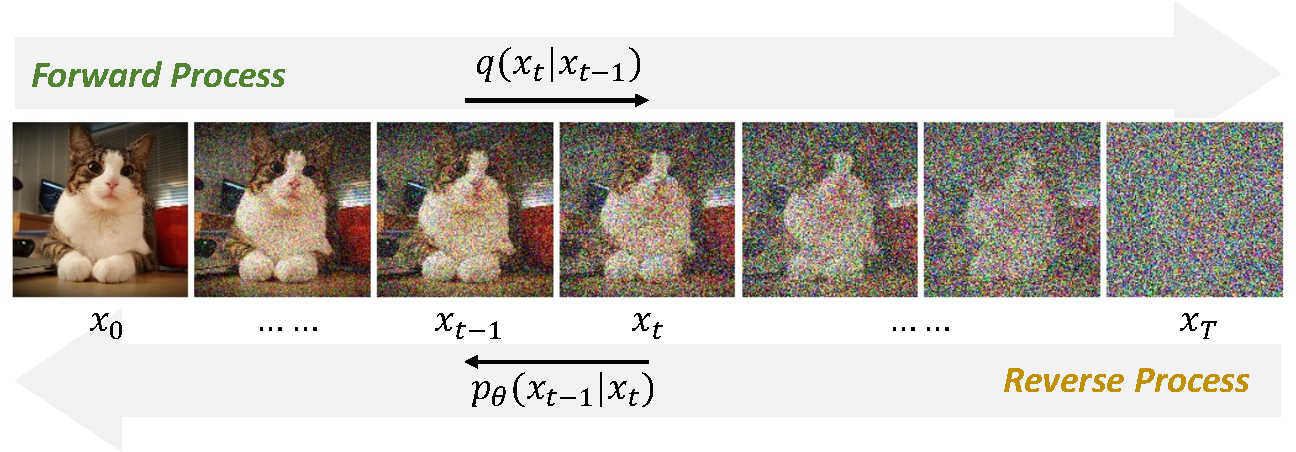
\includegraphics[width=1.0\textwidth]{img/diff_process.pdf}
	\caption{Forward and reverse process of diffusion model using 2D image as example, cat images are adapted from \cite{xiao2022DDGAN}.}
	\label{img:diff_process}
\end{figure}

\subsubsection{Conditional Diffusion Model}\label{sec:cond}
Conditional diffusion, also called guided diffusion is very practical in many applications since we normally want to generate the data in a particular style, direction or distribution and not in an arbitrary way. Typical usage of conditional diffusion is to sample data from a given class or category, as well as text prompt, image prompt and so on.

Mathematically, condition means the prior distribution $p(\mathbf{x})$ is conditioned on a given input $y$. By modifying the equation \ref{eq:reverse_all}, we get:
\begin{align}
  p_{\theta}(\mathbf{x}_{0:T}|y) = p_{\theta}(\mathbf{x}_{T})\prod_{t=1}^{T}p_{\theta}(\mathbf{x}_{t-1}|\mathbf{x}_{t},y)
\end{align}
Using the idea of the score-based generative model \cite{song2020generative}, we can train a score network for an unconditioned diffusion with the score function:
\begin{align}
  \mathbf{s}_{\theta}(\mathbf{x}_{t}, t)\approx \nabla _{\mathbf{x}_{t}}\log p_{\theta}(\mathbf{x}_{t})
\end{align}
Extend the score function with condition $y$, we can get the conditional score function after applying Bayes' Rule:
\begin{align}
  \nabla _{\mathbf{x}_{t}}\log p_{\theta}(\mathbf{x}_{t}|y)=\nabla _{\mathbf{x}_{t}}\log p_{\theta}(\mathbf{x}_{t}) + \nabla _{\mathbf{x}_{t}}\log p_{\theta}(y|\mathbf{x}_{t})
\end{align}
Based on the score function we can derive the conditional diffusion model with two variations, namely the classifier guidance and classifier-free guidance.

Classifier guidance is a method that balances the trade-off between mode coverage and sample fidelity post-training. It combines the score estimate of a diffusion model with the gradient of an image classifier, which requires training a classifier $f_{\phi}$ separate from the diffusion model and uses the gradients of the classifier as the guidance.

Without the separate classifier $f_{\phi}$, it is still possible to let the conditional and unconditional score functions share the same network, which is called classifier-free guidance. The diffusion model is trained by randomly dropping the condition $y$ during training. The result turns out to be that the conditional and unconditional score estimates are combined to attain a good tradeoff between quality and diversity \cite{ho2022classifierfree}.

The training and sampling algorithm of the conditional denoising diffusion probabilistic model can be summarized as the following algorithm \ref{algo:ddpm_train} and \ref{algo:ddpm_sample}.
\begin{algorithm}[H]
  \caption{Training of Conditional Diffusion Model}
  \label{algo:ddpm_train}
  \begin{algorithmic}[1]
    \Repeat
      \State $\mathbf{x}_{0}\sim q(\mathbf{x}_{0})$, conditional input $y$
      \State $t\sim \text{Uniform}(\{1,...,T\})$
      \State $\mathbf{\epsilon}\sim \mathcal{N} (\mathbf{0}, \mathbf{I})$
      \State Take a gradient descent step on $\nabla_{\theta}\left\lVert\boldsymbol{\epsilon} - \boldsymbol{\epsilon}_{\theta}(\sqrt{\bar{\alpha}_{t}}\mathbf{x}_{0} + \sqrt{1 - \bar{\alpha}_{t}}\boldsymbol{\epsilon}, t, y)\right\rVert ^{2}$ 
    \Until converged
  \end{algorithmic}
\end{algorithm}
\begin{algorithm}[H]
  \caption{Sampling of Conditional Diffusion Model}
  \label{algo:ddpm_sample}
  \begin{algorithmic}[1]
    \State $\mathbf{x}_{T}\sim \mathcal{N} (\mathbf{0}, \mathbf{I})$
    \For{$t=T$ to $1$}
      \State $\mathbf{z}\sim \mathcal{N} (\mathbf{0}, \mathbf{I})$ if $t>1$, else $\mathbf{z} = \mathbf{0}$
      \State $\mathbf{x}_{t-1}=\frac{1}{\sqrt{\alpha_{t}}}\left(\mathbf{x}_{t} - \frac{1-\alpha_{t}}{\sqrt{1-\bar{\alpha}_{t}}}\epsilon_{\theta}(\mathbf{x}_{t},t,y)\right) + \sigma_{t}\mathbf{z}$
    \EndFor
    \State \Return $\mathbf{x}_{0}$
  \end{algorithmic}
\end{algorithm}

\subsection{Applications}

\subsubsection{Computer Vision}
The majority of the applications of diffusion models lie in the field of computer vision, including super-resolution, translation, inpainting and so on  \cite{yang2023diffusion}. Diffusion models have shown a great performance in these \gls{2d} based manipulation tasks compared with other generative models such as \glspl{gan} and \glspl{vae}.

\gls{sr3} \cite{saharia2021image} and \gls{cdm} \cite{ho2021cascaded} are two representative works in the field of super-resolution. They use either an iterative way or a concatenation of diffusion models to generate high-resolution images from low-resolution inputs. Figure \ref{img:sr3} illustrates the process of cascaded super-resolution, which is taken from the project page of the \gls{sr3}. \gls{idm} for Continuous Super-Resolution \cite{gao2023implicit} integrates an implicit neural representation in the decoding process.

Inpainting and image translation are also two popular image manipulation tasks with different conditional inputs. Typical works are RePaint \cite{lugmayr2022repaint}, Palette \cite{saharia2022palette} and Diffusion-based Image Translation using Disentangled Style and Content Representation \cite{kwon2023diffusionbased}.
\begin{figure}[h]
	\centering
	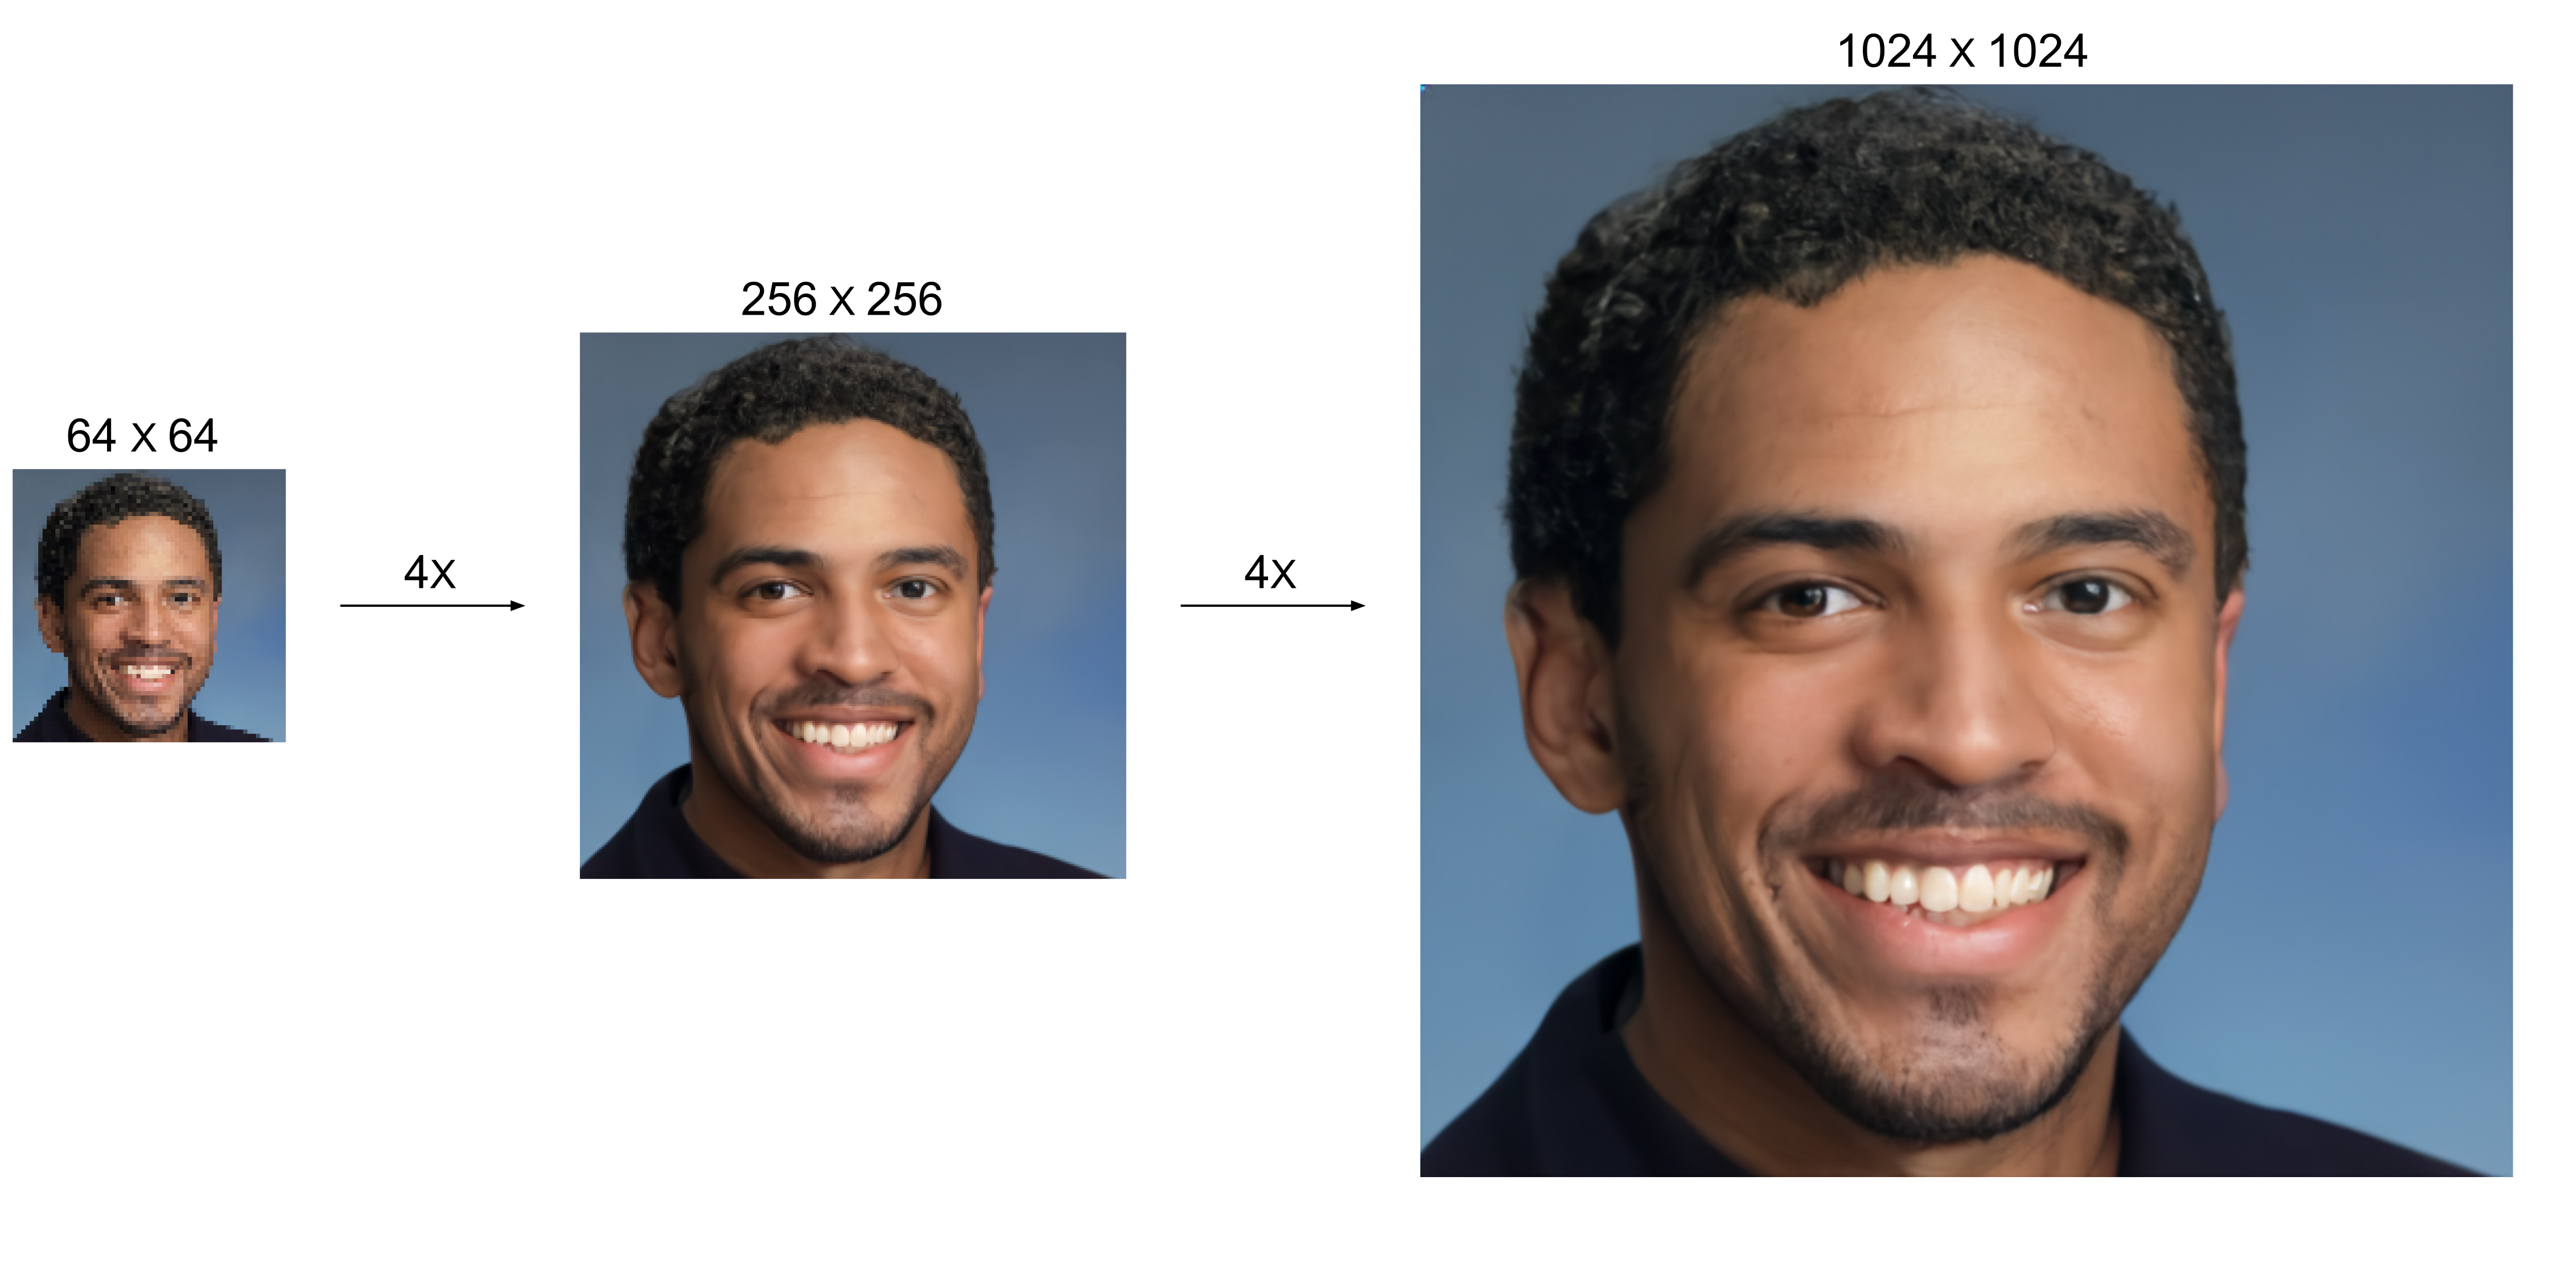
\includegraphics[scale=.08]{img/cascade_fig.png}
	\caption{Super resolution using diffusion model, image taken from the project page of SR3 \cite{saharia2021image}.}
	\label{img:sr3}
\end{figure}


In \gls{3d} domain, the diffusion model is also applied to the task of point cloud generation and completion. Luo et al.2021 \cite{luo2021diffusion} and Zeng et al.2022 \cite{zeng2022lion} have presented the diffusion models for point cloud generation by treating point clouds as particles in a thermodynamic system. Lyu et al.2022 \cite{lyu2022conditional} have proposed a coarse-to-fine point cloud completion diffusion model and also established a point-wise mapping between the output and ground truth. Figure \ref{img:pcd} adapted from the paper shows the point cloud generation using diffusion architecture.

\begin{figure}[h]
	\centering
	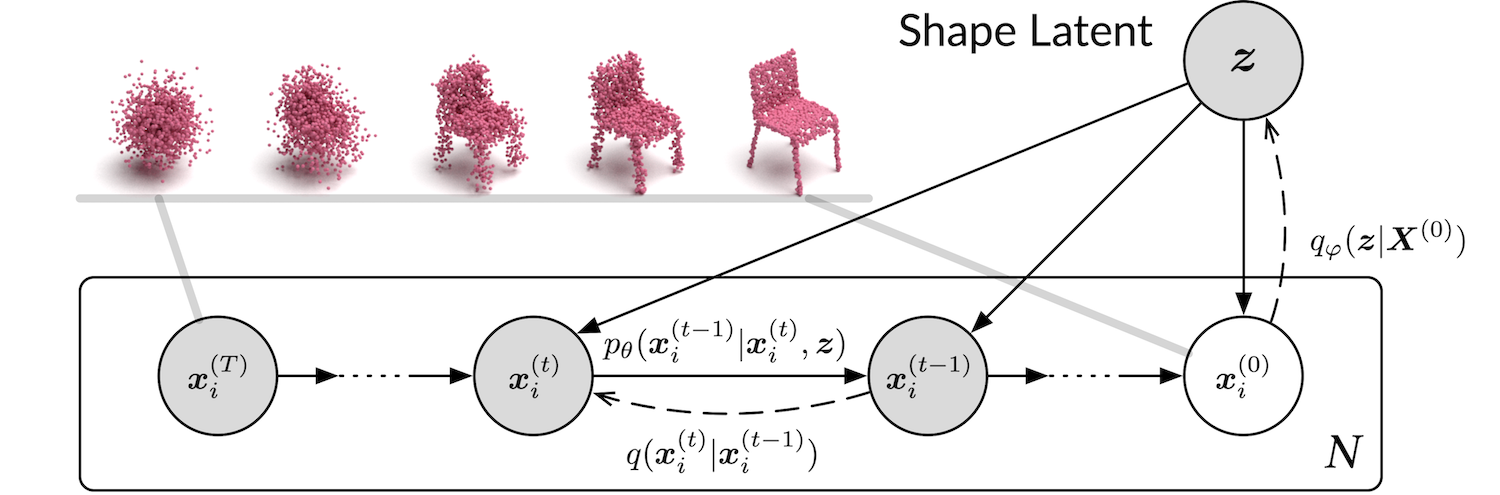
\includegraphics[scale=1.8]{img/teaser.png}
	\caption{Point cloud generation using diffusion model, image taken from \cite{lyu2022conditional}.}
	\label{img:pcd}
\end{figure}


\subsubsection{Natural Language Processing}
\gls{nlp} has been dramatically developed in recent years. The iconic models like BERT \cite{devlin2019bert}, GPT series \cite{Radford2018ImprovingLU} and LLaMA \cite{touvron2023llama} are all based on the Transformer architecture. However, some diffusion-based methods can generate text with high quality and diversity. In fact, diffusion models have been shown to have significant advantages over autoregressive models in terms of parallel generation, text interpolation, token-level controls such as syntactic structures and semantic contents, and robustness \cite{zou2023survey}.

\gls{d3pm} \cite{austin2023structured}, is a diffusion-like generative model for discrete data that generalizes the multinomial diffusion model \cite{hoogeboom2021argmax}, by going beyond corruption processes with uniform transition probabilities. 

Diffusion-LM \cite{li2022diffusionlm} proposes a non-autoregressive language model based on continuous diffusions, which iteratively denoises a sequence of Gaussian vectors into word vectors, yielding a sequence of intermediate latent variables, which makes it possible for simple, gradient-based methods to achieve complex control.
\subsubsection{Multi-Modal Learning}
Multi-modal learning is a field that combines different modalities such as text, image, video and audio. It tends to become the mainstream of future research in the field of machine learning because of the higher requirement of real-world applications.

Text-to-image generation is a typical task in this field. A common pipeline is to first train a prior model that can generate image embedding conditioned on a text prompt,e.g. CLIP \cite{radford2021learning}. Then we use the prior output as a condition to train a diffusion model to generate the final image. Famous works like Stable Diffusion \cite{rombach2022highresolution} and DALLE-2 \cite{ramesh2022hierarchical} followed this pipeline and achieved state-of-the-art results in text-to-image generation. Following Text-to-Image samples \ref{img:sd} are generated using Stable Diffusion.

\begin{figure}[h]
	\centering
	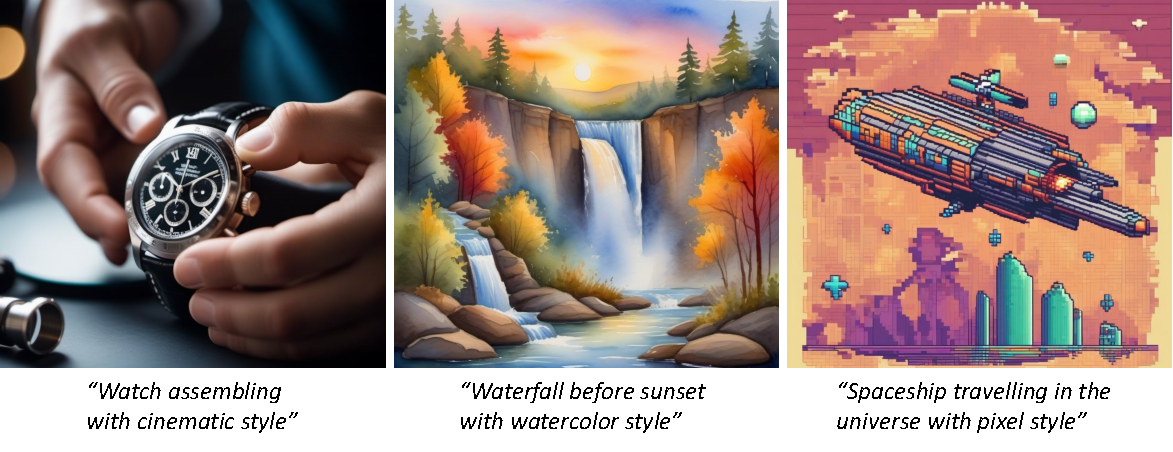
\includegraphics[width=1.0\textwidth]{img/sd.pdf}
	\caption{Image synthesis with text prompt in different styles using Stable Diffusion \cite{rombach2022highresolution}.}
	\label{img:sd}
\end{figure}

ControlNet \cite{zhang2023adding} attempts to control pre-trained large diffusion models to support additional semantic maps, like edge maps, segmentation maps, key points, shape normals, depths, etc. The authors use the "trainable copy" of the original weights of the pre-trained diffusion model and connect these "copy" blocks in the original model with zero convolution layers. Thus, we don't need to retrain the whole model and also guarantee the quality as well as the flexibility of the model.

Text-to-\gls{3d} generation and Image-to-\gls{3d} are novel tasks in the field of multi-modal learning and have the potential to be applied in many cases such as \gls{3d} object reconstruction, \gls{3d} scene generation and so on. DreamFusion \cite{poole2022dreamfusion} adopts a pre-trained \gls{2d} text-to-image diffusion model to perform text-to-\gls{3d} synthesis. It optimizes a randomly-initialized \gls{3d} model based on \gls{nerf} with a probability density distillation loss, which utilizes a \gls{2d} diffusion model as a prior for optimization of a parametric image generator. Figure \ref{img:df} illustrates the process of the text-to-\gls{3d} generation using DreamFusion, and the image is adapted from the demo in the original work.

\begin{figure}[h]
	\centering
	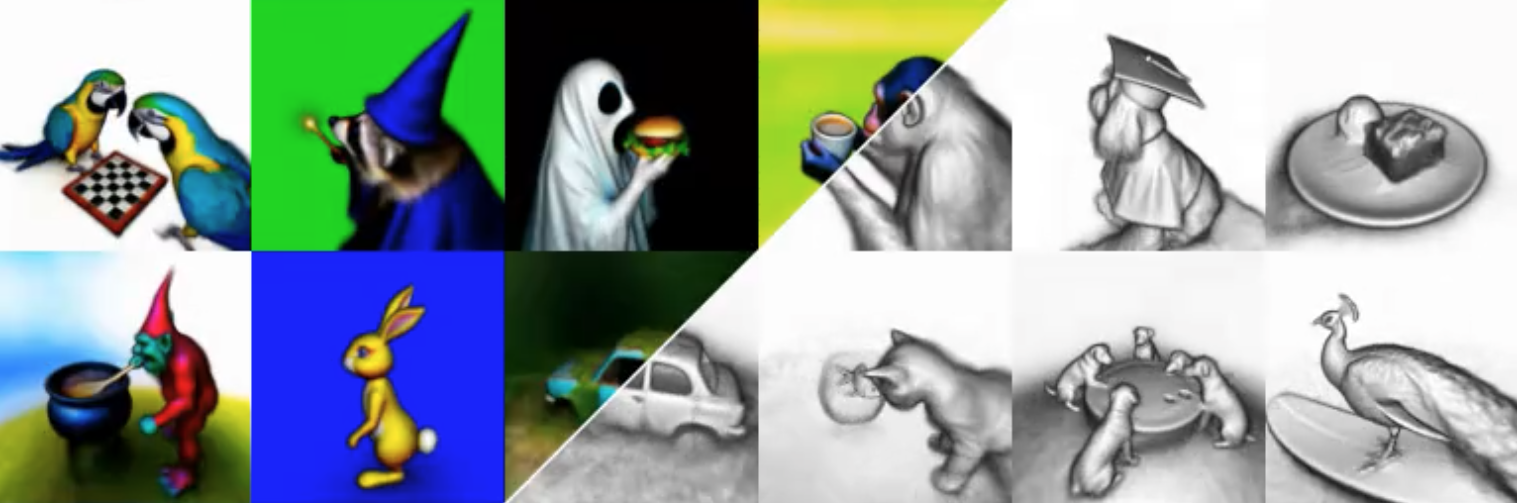
\includegraphics[width=1.0\textwidth]{img/df.png}
	\caption{3D model NeRF synthesis prompt using DreamFusion, image taken from \cite{poole2022dreamfusion}.}
	\label{img:df}
\end{figure}

\chapter{Related Works}
\section{6 DoF Pose Estimation}
\subsection{Learning-Free Methods}
In the early stage of the \gls{6dof} pose estimation research, the methods are mainly based on the hand-crafted feature descriptors such as \gls{sift} \cite{sift}, \gls{surf} \cite{surf} and \gls{orb} \cite{6126544}. The main idea of these methods is to extract the feature points from the image and find the \gls{2d}-\gls{3d} correspondences. After that, the pose of the object can be estimated by solving the \gls{pnp} problem. The \gls{pnp} problem is a classic problem in computer vision which is to estimate the pose of an object given a set of \gls{3d} points in the object coordinate system and the corresponding \gls{2d} projections in the image plane. The \gls{pnp} problem can be solved by using the \gls{ransac} \cite{10.1145/358669.358692} algorithm to find the inliers and then use the least square method to estimate the pose. The main drawback of these methods is that they are sensitive to occlusion, texture-less objects and illumination change. 

\gls{icp} \cite{Besl1992AMF} and its improved version such as \gls{gicp} \cite{gicp} and \gls{nicp} \cite{nicp} are also used to estimate the pose of the object when the depth information (point cloud) is available as reference. The task is also called point cloud registration where a partial point cloud is registered to a complete one or the alignment between two \gls{3d} scenes is estimated. However, the \gls{icp} is basically a time-consuming iterative method that is sensitive to the initial pose and the convergence is not guaranteed. Using \gls{icp} alone is not sufficient to achieve a robust pose estimation, but it can be used as a post-processing method to refine the pose estimation at the coarse level. The optional \gls{icp} module as the learning-free algorithm can effectively reduce the residual error existing in the learning-based methods and improve the final accuracy. In our framework, we also adapt the \gls{icp} as our refinement to further boost the performance.
\subsection{Template-Based Methods}
Template-based methods have been widely used to handle the texture-less object in the pose estimation task. In \gls{2d} object detection, a template is created from the object of interest and we scan the reference image with the template to locate the object. Adapting the same idea, in \gls{6dof} pose estimation a template is usually rendered from the \gls{3d} \gls{cad} model of the object and the pose of the object can be estimated by calculating the similarity score between the template and the reference image. 

Gu et al. 2010 \cite{gu2010discriminative} propose to use a mixture of holistic templates and discriminative learning for joint object categorization and viewpoint classification. Different objects are learned in the mixture and related to the canonical viewpoints with different supervision strategies. Hinterstoisser et al. 2012 \cite{hinterstoisser2012gradient} confront the time-consuming shortcoming of the template-based methods by using the gradient response maps and we only need to test a subset of all possible pixel locations. Wohlhart et al. 2015 \cite{Wohlhart_2015} provide a powerful approach to compute the descriptors for object views which memorize both object class and pose information. The scalable nearest neighbor search is utilized to handle a large number of objects as well as viewpoints. Generalization of the template-based problem is emphasized in the recent work from Nguyen et al. 2022 \cite{nguyen2022templates} and increases the robustness against the occlusion and cluttered background by using the \gls{cnn}-based feature extraction. A similar idea is used in OSOP \cite{shugurov2022osop}, which is a one-shot method combining template matching with dense \gls{2d}-\gls{3d} correspondence prediction. Additional \gls{pnp}+\gls{ransac} or Kabsch \cite{kabsch1976solution}+\gls{ransac} and pose hypothesis verification are used to further refine the pose estimation.
\subsection{Keypoint-Based Methods} 
Instead of directly estimating the pose from the reference input, keypoint-based methods first detect the key points or super points in the reference image and then solve the correspondence matching problem between the \gls{rgb} image and the \gls{3d} model by \gls{pnp}. In the case of point cloud registration, the task becomes to find the correspondences between the partial point cloud and the \gls{3d} model.

\gls{rgb}-only keypoint matching is the most common method because the \gls{2d} data is more accessible than the data with additional depth information and the networks dealing with \gls{2d} image are more mature as well. Besides the hand-crafted feature descriptor that we introduced before, methods like \cite{pavlakos20176dof, rad2018bb8, pmlr-v87-tremblay18a,tekin2018realtime, zakharov2019dpod} use the \gls{cnn}-based architecture to extract the \gls{2d} semantic keypoints and estimate the pose by \gls{pnp} algorithm. Especially, Oberweger et al. 2018 \cite{oberweger2018making} propose a \gls{rgb}-only method that can estimate the pose under large occlusion. Their solution is to predict heatmaps from multiple patches independently and calculate the accumulated score to ensure a robust estimation. ZebraPose \cite{su2022zebrapose} assigns a hierarchical binary grouping to encode the object surface. It replaces the sparse correspondence matching with dense maps learning to handle the occluded object and make the learning of \gls{2d}-\gls{3d} correspondences more efficient.

With the promising performance of the \gls{3d} networks \cite{qi2017pointnet,qi2017pointnet++} in recent years, some methods are proposed to directly tackle the \gls{3d} key points in the pose estimation task. D3Feat \cite{bai2020d3feat} leverage a \gls{3d} \gls{cnn}-based architecture to jointly learn the detection and description of \gls{3d} local features. SpinNet \cite{ao2021spinnet} aims to learn efficient descriptors which are rotationally invariant. The Spatial Point Transformer is introduced to map the local surface into a cylindrical space for end-to-end optimization with $\mathbb{SO}(2)$ equivariant representation. YOHO \cite{wang2022hypothesize} is another work that ensures the rotation invariance with the help of group equivariant feature learning. The novel descriptors make the correspondence matching more accurate and fewer \gls{pnp} iterations are needed. GeoTransformer \cite{qin2022geometric} leverages the efficient local feature extraction by using the geometrical embedding and follows the coarse-to-fine pipeline to achieve \gls{ransac}-free pose estimation. The enhanced version of this work, RolTr \cite{yu2023rotationinvariant} further improved the performance by utilizing the local-to-global attention-based rotation-invariant feature learning. And it outperforms the state-of-the-art methods in the low-overlapping scenarios.


\subsection{Direct Regression Methods}
Another popular group of \gls{6dof} pose estimation methods follows an end-to-end pipeline which requires the estimation process to be differentiable.

PoseCNN \cite{xiang2018posecnn} is an early research that leverages the \gls{cnn} on \gls{2d} image. It estimates the translation through the object center with the distance to the camera and regresses the quaternion representation of rotation. The symmetrical object is also considered by introducing a novel loss function of the rotation. Similar work from Wu et al. 2018 \cite{Wu_2018} trains a \gls{cnn}-based model only on the synthetic data instead of expensively annotated object pose data. They overcome the domain gap between real and synthetic data by using object masks as an intermediate representation. Deep-6DPose \cite{do2018deep6dpose} extends the instance segmentation network Mask \gls{rcnn} \cite{he2018mask} and decouples the translation and rotation to make the rotation be regressed in Lie algebra representation. GDR-Net \cite{wang2021gdrnet} is a novel method that directly regresses the \gls{6dof} pose from the \gls{rgb} data in an end-to-end manner. It takes the zoomed-in region of interest as input and predicts hierarchical intermediate geometric features. Then the pose is regressed from the introduced tricks of Dense Correspondances and Surface Region Attention.

Direct regression of the transformation between two point clouds is more straightforward than the correspondence-based method in the point cloud registration task. PointNetLK \cite{aoki2019pointnetlk} combines the PointNet in \gls{3d} domain with the Lucas \& Kanade algorithm \cite{Lucas1981AnII} for \gls{2d} image alignment together to regress the transformation between two frames. Huang et al. 2020 \cite{huang2020featuremetric} propose a method that optimizes the registration by minimizing a feature-matrix projection error without matching the correspondence. OMNet \cite{xu2021omnet} is another global feature-based iterative network for partial-to-partial registration. It utilizes overlapping masks to reject non-overlapping regions, transforming partial registration into same-shape registration.

Thanks to the decreasing cost of \gls{rgbd} sensor in recent years, \gls{rgb} data with additional depth information enable us to more precisely handle texture-less objects in poorly illuminated scenarios. Some \gls{rgbd} based dense methods are proposed to estimate the pose in a fine-grained way. Kehl et al. 2016 \cite{kehl2016deep} use regressed descriptors of locally sampled patches with a convolutional auto-encoder and then cast 6D voting for each patch to estimate the pose. Pix2Pose \cite{Park_2019}, PVNet \cite{peng_pvnet_2019} and \gls{df} \cite{wang2019densefusion} are typical pixel-wise regression methods, where gls{df} is a representative method that pixel-wise votes the \gls{6dof} pose prediction. The network concatenates the \gls{2d} feature extracted from \gls{cnn} and the \gls{3d} feature from PointNet together with the global feature through average pooling. The pixel-wise dense predictions are voted through the trainable confidence for each pixel. And FFB6D \cite{he2021ffb6d} as its successor, builds a bidirectional network to enhance the feature fusion from both domains. HybridPose \cite{song2020hybridpose} utilizes more information from the image like key points, edge vectors and symmetry correspondences to achieve more diverse feature representation for regression.

Common structures of \gls{6dof} pose estimation methods are summarized in the following figure \ref{img:pose_methods}.
\begin{figure}[h]
	\centering
	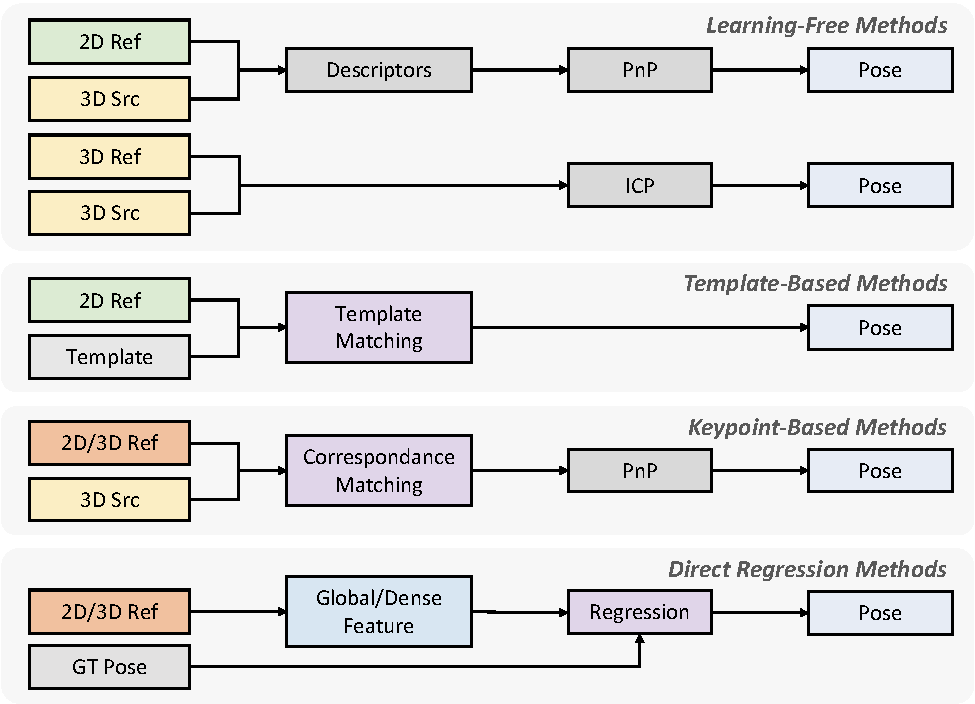
\includegraphics[width=1.\textwidth]{img/pose_methods.pdf}
	\caption{Structures of some common 6 DoF pose estimation methods.}
	\label{img:pose_methods}
\end{figure}

\section{Diffusion Models}
\subsection{Foundations}
Besides the original \gls{ddpm} \cite{sohldickstein2015deep,ho2020denoising} which is introduced in section \ref{sec:theory}, another two fundamental models of all works based on diffusion models are the \glspl{sgm} \cite{song2020generative,song2020improved} and \glspl{sde} \cite{song2021maximum,song2021scorebased}.

The concept of SGMs is to use the Stein-score function to optimize the estimated distribution. The score $\nabla_{\mathbf{x}}log p(\mathbf{x})$ is defined as the gradient of the log-density of the \gls{pdf} $p(\mathbf{x})$. It represents a vector field that points in the direction of the steepest ascent of the \gls{pdf}. The advantage of the score-based model is that we can parameterize the model without considering the normalization constant of the \gls{pdf} by the operation of the derivative. That means we don't need any special treatment to make the normalizing constant trackable compared with the likelihood-based models. The training of the score-based models is to minimize the Fisher divergence between the model and the data distribution, which is defined as:
\begin{align}\label{eq:sgm}
  D_{F} = \mathbb{E}_{p(\mathbf{x})}\left[\left\lVert\nabla_{\mathbf{x}}\log p(\mathbf{x}) - \mathbf{s}_{\theta}(\mathbf{x})\right\rVert^{2}\right]
\end{align}
where $\nabla_{\mathbf{x}}log p(\mathbf{x})$ is hard to track in practice because we don't have the knowledge of the data distribution $p(\mathbf{x})$. However, we can utilize the method of score matching \cite{10.5555/1046920.1088696,6795935} to minimize the Fisher divergence without knowing the ground truth score of the data.

The likelihood-based or score-based diffusion models can be further extended from the fixed step size to the continuous time domain using the \glspl{sde}. Perturbing the data distribution with a continuously developing noise following the \glspl{sde} process, we have the following equation:
\begin{align}
  \text{d}\mathbf{x}=\mathbf{f}(\mathbf{x},t)dt + g(t)\text{d}\mathbf{w}
\end{align}
where $\mathbf{f}(\mathbf{x},t)$ is called drift term and $g(t)$ is the diffusion coefficient, $\mathbf{w}$ is a standard Wiener process (or Brownian motion). The forward processes of \glspl{ddpm} and \glspl{sde} have the discrete version of the continuous-time \glspl{sde}. And the corresponding reverse \gls{sde} can be represented as:
\begin{align}
  \text{d}\mathbf{x}=\left[\mathbf{f}(\mathbf{x},t)-g^{2}(t)\nabla_{\mathbf{x}}log p_{t}(\mathbf{x})\right]\text{d}t + g(t)\text{d}\mathbf{w}
\end{align}
where $p_{t}(\mathbf{x})$ is the density of the data distribution at time $t$. After that, the time-based training objective can be formulated with modification from equation \ref{eq:sgm} as:
\begin{align}
  D_{F} = \mathbb{E}_{t\in \mathcal{U}(0,T)} \mathbb{E}_{p_{t}(\mathbf{x})}\left[\lambda(t)\left\lVert\nabla_{\mathbf{x}}log p_{t}(\mathbf{x}) - \mathbf{s}_{\theta}(\mathbf{x},t)\right\rVert^{2}\right]
\end{align}
where $\mathcal{U}(0,T)$ is a uniform distribution over the interval $[0,T]$ and $\lambda(t)$ is a weighting function that is used to balance the contribution of each timestep. The \glspl{sde} based diffusion models are more flexible and can be applied to the continuous-time domain, which is more fine-grained than the discrete-time models.
\subsection{Improvements on Sampling}\label{sec:impr_sample}

The sampling process of the original diffusion models takes a large amount of time because of its iterative architecture during the reverse process. In order to improve the efficiency of the sampling process, some work has been done to accelerate the sampling process.
\subsubsection{Learning-Free Sampling}
The first group of methods can be categorized as learning-free sampling. The main works of the advanced sampler focus on the efficient discretizing of the time-continuous solver. The \gls{sde}-based sampler such as \gls{cas} \cite{jolicoeurmartineau2020adversarial} which is improved from \gls{ald} \cite{dockhorn2022scorebased} proposes a modified \gls{sde} with consistent scaling of the added noise and ensures the expected geometric progression of the noise and make the generated samples closer to the data distribution. Another work from Jolicoeur-Martineau et al. 2021 \cite{jolicoeurmartineau2021gotta} introduces a new \gls{sde} solver with adaptive step size controlled by comparing the high-order and low-order \gls{sde} solvers' outputs.

There are also many methods that rely on the \glspl{ode} solver. Song et al. 2021 \cite{song2021scorebased} states the probability flow \gls{ode} with the marginals same as the reverse-time \gls{sde}. The \gls{ode} solvers are deterministic, therefore the convergence is much faster than the stochastic solvers with the small tradeoff of the sample quality. \gls{ddim} \cite{song2022denoising} is the pioneer of the work in this field, which extends the \gls{ddpm} to non-Markovian perturbation. Karras et al. 2022 \cite{karras2022elucidating} propose a sampling process using Heun's $2^{\text{nd}}$ order method. DPM-Solver \cite{lu2022dpmsolver} is a fast dedicated high-order solver for diffusion \glspl{ode} with the convergence order guarantee. The advanced \gls{ode} solver makes the sampling process much faster than \gls{ddim} and also improves the sample quality.

\subsubsection{Learning-Based Sampling}
Another sampling strategy is called learning-based sampling. By training the reverse process, the sampler is able to select the critical steps so that the training objective can be efficiently optimized. Watson et al. 2021 \cite{watson2021learning} introduce an exact dynamic programming algorithm that finds the optimal discrete-time schedules for any pre-trained \gls{ddpm}. After that, \gls{ddss} \cite{watson2022learning} is proposed to accelerate the sampling by differentiating through sample quality scores. 

Instead of optimizing the schedule of the sampling process, works like Early-Stopped \gls{ddpm} \cite{lyu2022conditional} and Truncated \gls{ddpm} \cite{zheng2023truncated} propose to train the diffusion model without the complete forward and start the denoising from a non-gaussian distribution, so that the denoising steps can be significantly reduced. Another approach is to utilize the knowledge distillation \cite{salimans2022progressive,meng2023distillation} to compress the sampling steps into just a few steps. Progressive Distillation, for example, is able to reduce the steps from over a thousand to four steps without losing much sample quality by progressively parameterizing the sampler.
\subsection{Improvements on Likelihood}
Original \gls{ddpm} need to optimize the variational \gls{elbo} because of the intractable log-likelihood (see section \ref{sec:reverse}). When we use time-continuous diffusion such as \glspl{sde}, some methods are proposed to estimate the likelihood of the data distribution. Song et al. 2021 \cite{song2021maximum} realize a connection between the maximum likelihood estimation with the weighted combination of score matching with a specific weighting scheme. \gls{vdm} \cite{kingma2023variational} introduce a simplification of the time-continuous variational lower bound which is invariant to the noise schedule and accelerates the optimization. Besides combining the score matching the maximum likelihood estimation, Nichol et al. 2021 \cite{nichol2021improved} propose a hybrid way to define the training objective by adding the variational lower bound with the score matching loss with a control parameter $\lambda$.

\subsection{Extended Data Structures}
Most of the works based on diffusion models focus on the \gls{2d} image generation and manipulation tasks, where the data is continuous in \gls{2d} space. However, there is also some work that applies diffusion models to other data structures such as text, graphs, point clouds and so on. The standard method of the diffusion model may not be suitable for these data structures, so some modifications are needed to adapt the diffusion model to different data structures.
\subsubsection{Discrete Data}
To adapt the perturbation of the Gaussian noise to the discrete data, some works extend the original \gls{ddpm} to the discrete domain, especially in \gls{nlp} field. For instance, VQ-Diffusion \cite{gu2022vector} inspired from \gls{vqvae} \cite{oord2018neural} replaces the Gaussian noise with a mask-and-replace diffusion strategy to avoid the accumulation of error, which is the first application of diffusion model on vector-quantized data. \gls{csm} \cite{meng2023distillation} proposes an analogous score function called "Concrete score", which is a generalized Stein score for discrete data. It is defined by the rate of change of the probabilities with respect to local directional changes of the input. Liu et al. 2023 \cite{liu2023learning} propose a method dealing with the data on constrained and structured domains, including discrete data as a special case. The diffusion model is driven by a drift force that is a sum of two parts: one singular force designed by Doob's h-transform that enforces the outcome in the constrained domain, and one non-singular neural force field that ensures statistical consistency.
\subsubsection{Manifold}
In many real-world applications, data lies in the non-Euclidean space. For instance, the Riemannian manifolds are widely used in the robotic and computer vision field. \gls{rdm} \cite{huang2022riemannian} generalizes continuous-time diffusion models to arbitrary Riemannian manifolds and derives a variational framework for likelihood estimation. Similar work like \gls{rsgm} \cite{debortoli2022riemannian} extends the SGMs to the setting of compact Riemannian manifolds.

Graph structure is also a common data structure that represents the relationship between different entities which is an efficient expression in fields like data mining,  protein structure prediction and so on. Niu et al. 2020 \cite{niu2020permutation} first propose a permutation invariant equivariant graph neural network called EDP-GNN and integrate it into the score-based generative model. Graph-GDP \cite{huang2022graphgdp} further constructs a forward diffusion process with a \gls{sde}, which perturbs the graph with a known edge probability. A position-enhanced graph score network is trained to extract the structure and position information from the graph for permutation equivariant score estimation.

The majority of the raw data lie in the high-dimensional space but can be represented in the low-dimensional manifold using a network like autoencoder. And working on these latent spaces is more efficient and effective. For this reason, some recent works utilize the diffusion model on the manifold which is compressed from the original data space. The \gls{lsgm} \cite{vahdat2021scorebased} proposes a method to jointly train a score-based diffusion model and a variational autoencoder by optimizing the ELBO of the \gls{vae} together with the training objective of the score matching model. Instead of the joint training, \gls{ldm} \cite{rombach2022highresolution} used in the influential work of Stable Diffusion, addresses the training into two separate phases. First, the autoencoder is trained to project the data into latent space. Then, the diffusion model is trained to directly sample the latent expression of the data.

\section{Diffusion models in Pose Estimation}
The objective is \gls{6dof} pose estimation lies on the $\mathbb{SE}(3)$ of Lie group, which is a differentiable manifold that is generalized from the Euclidean space. Recent works from Leach et al. 2022 \cite{leach2022denoising} first explore the usage of the diffusion model to generate the probability density on $\mathbb{SO}(3)$. Jagvaral et al. 2023 \cite{jagvaral2023diffusion} further optimized the loss function from the Euclidean space to the manifold $\mathbb{SO}(3)$. Urain et al. 2023 \cite{urain2023se3diffusionfields} propose smooth cost functions for joint grasp on $\mathbb{SE}(3)$ through diffusion. Yim et al. 2023 \cite{yim2023se3} introduce a framework called FrameDiff to learn the $\mathbb{SE}(3)$ equivariant score of the diffusion models over multiple frames in protein structure generation. 

Typical work from Hsiao et al. 2023 \cite{hsiao2023confronting} focuses on the advantages of diffusion models towards the pose ambiguity problem on $\mathbb{SE}(3)$. The denoiser backbone consists of several \gls{mlp} blocks processing the \gls{2d} global feature extracted from a pre-trained ResNet. Figure \ref{img:confront} shows the overview of the framework. The authors use the surrogate Stein score calculation on $\mathbb{SE}(3)$ following the score-based diffusion architecture and Fourier-based conditioning mechanism to deal with the ambiguity problem caused by the symmetrical object. Additionally, they also compare the advantage of $\mathbb{SE}(3)$ parametrization over previous works on $R^{3}\mathbb{SE}(3)$. This work is trained and evaluated on the synthetic dataset SYMSOL \cite{implicitpdf2021} with fice texture-less objects, namely tetrahedron, cube, icosahedron, cone, and cylinder. The denoising process is shown in figure \ref{img:confront_cube}. The real data captured by the camera is not considered in this work. In our proposed method, we focus on pose estimation with diffusion models under the real-world scenario and even with occlusion, which is more general and challenging.
\begin{figure}[h]
	\centering
	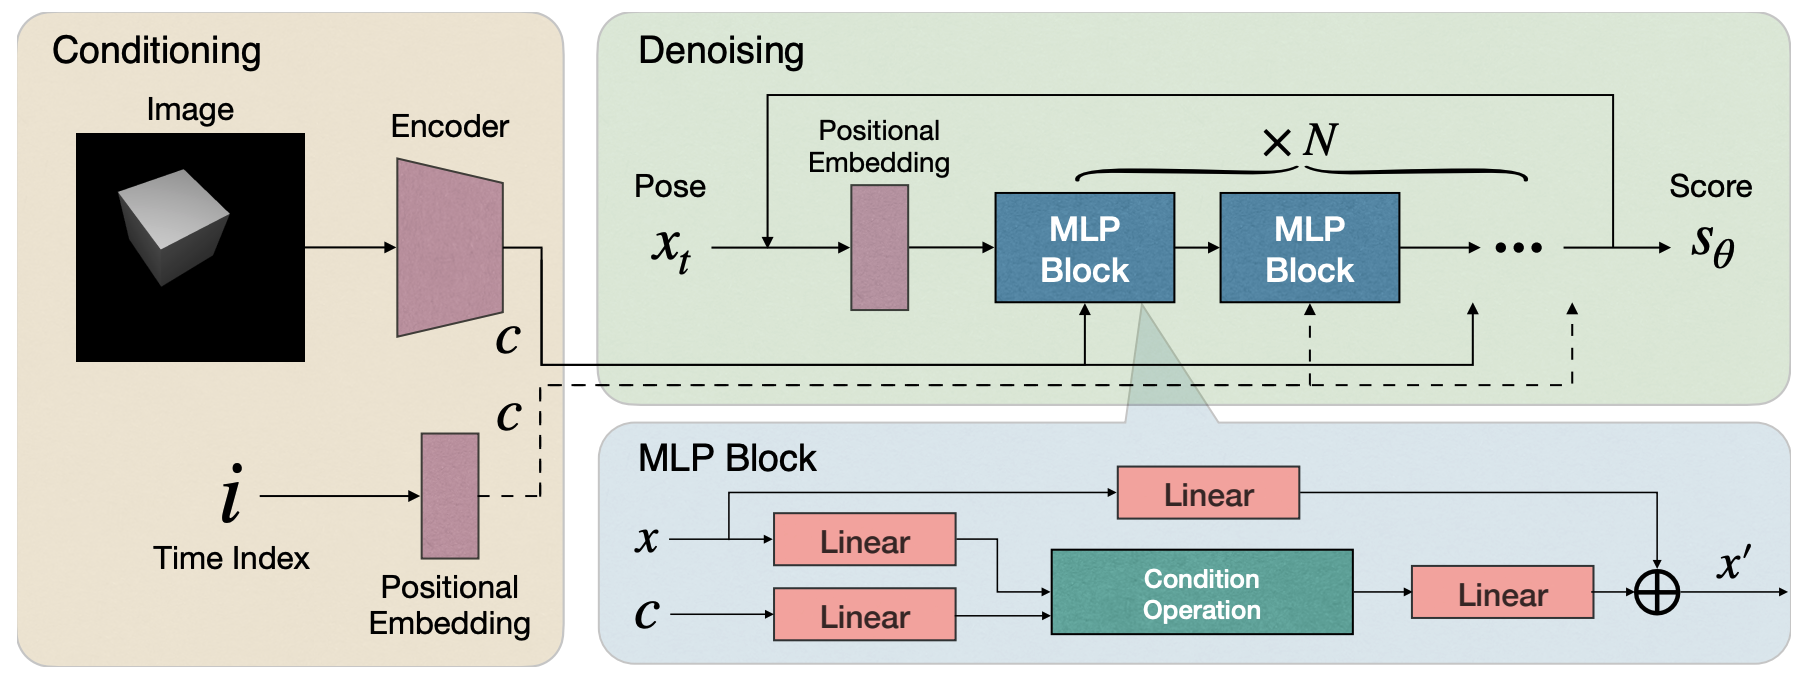
\includegraphics[width=1.\textwidth]{img/confront.png}
	\caption{Overview of the network from the work "Confronting Ambiguity in 6D Object Pose Estimation via Score-Based Diffusion on SE(3)", image adapted from the original paper \cite{hsiao2023confronting}.}
	\label{img:confront}
\end{figure}

\begin{figure}[h]
	\centering
	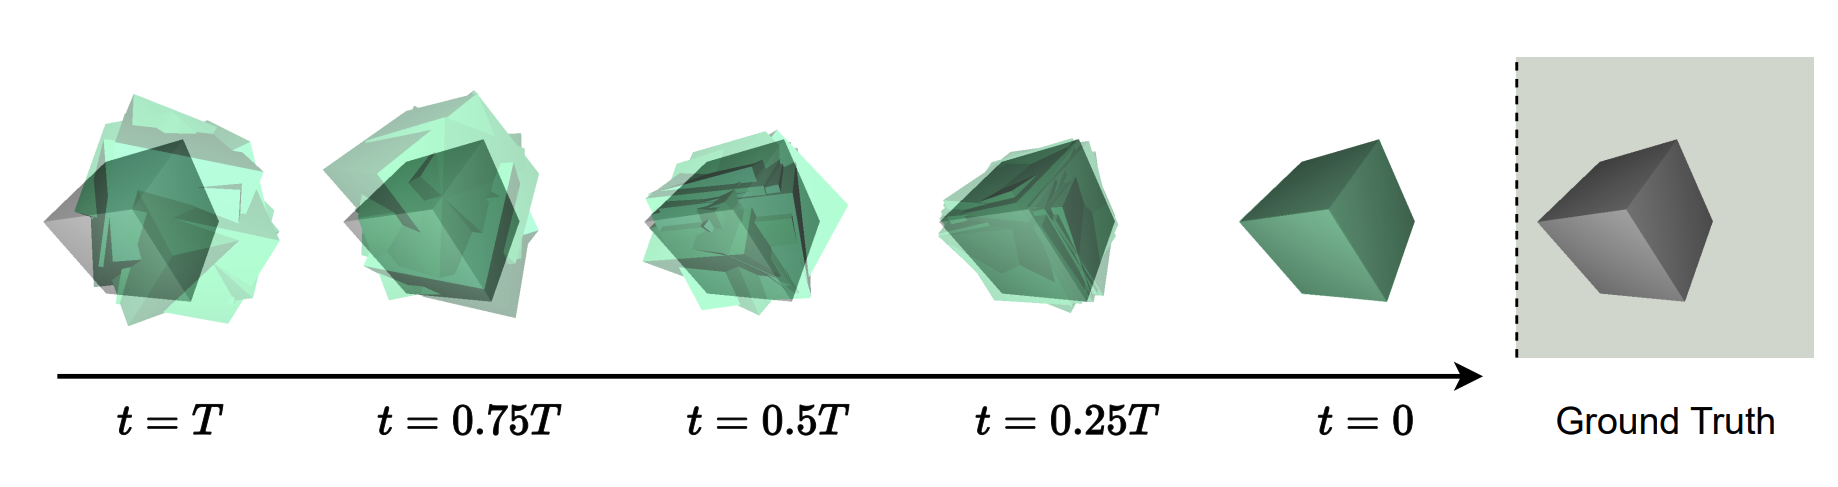
\includegraphics[width=1.\textwidth]{img/confront_cube.png}
	\caption{Visualisation of the denoising process from the work "Confronting Ambiguity in 6D Object Pose Estimation via Score-Based Diffusion on SE(3)", image adapted from the original paper \cite{hsiao2023confronting}.}
	\label{img:confront_cube}
\end{figure}

Wang et al. 2023 \cite{wang2023pd} propose a diffusion-aided bundle adjustment network for the camera pose estimation with a series of input images. Similar to the previous work, the diffusion network is conditioned by the \gls{2d} feature downstream by a pre-trained encoder. The highlight of this method is the geometry-guided sampling of the diffusion model with the Sampson epipolar error minimization so that the image-to-image epipolar constraint can be satisfied in the sampling phase. Figure \ref{img:pose_diff} and \ref{img:pose_diff_vis} illustrate the overview of the framework and the denoising process of the bundle adjustment. The model is evaluated on CO3Dv2 \cite{reizenstein2021common} containing turntable-like objects and RealEstate10K \cite{zhou2018stereo} which captures videos of the interior and exterior of real estate. Both datasets aim to estimate the camera poses with a series of input images relative to the object or the scene. Our work focuses on the single-frame object pose estimation with the fixed camera parameters and processes the data further with the depth information.

\begin{figure}[h]
	\centering
	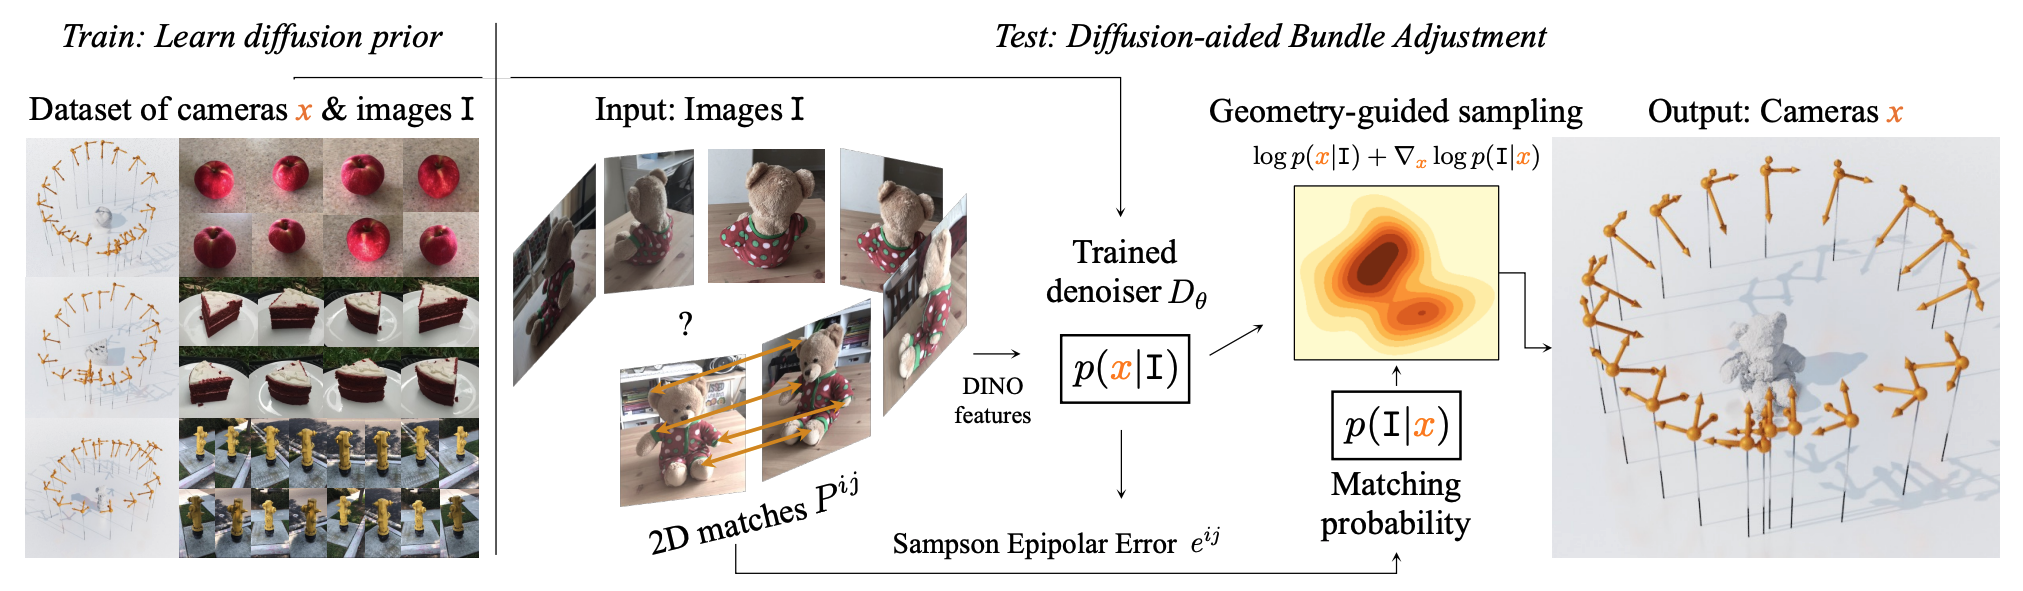
\includegraphics[width=1.\textwidth]{img/pose_diff.png}
	\caption{Overview of the network from PoseDiffusion, image adapted from the original paper \cite{wang2023pd}.}
	\label{img:pose_diff}
\end{figure}

\begin{figure}[h]
	\centering
	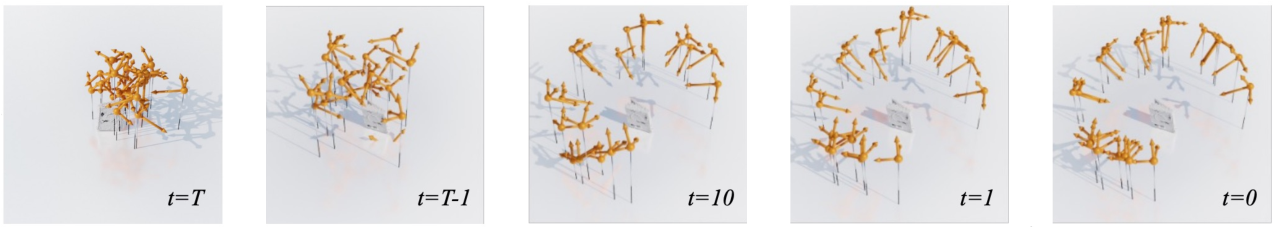
\includegraphics[width=1.\textwidth]{img/pose_diff_vis.pdf}
	\caption{Visualisation of the denoising process from PoseDiffusion, image adapted from the original paper \cite{wang2023pd}.}
	\label{img:pose_diff_vis}
\end{figure}

\chapter{Methodology}
\section{Introduction}
In this chapter, we will introduce the details of our proposed method, namely the pose hypotheses diffusion. The intuitive idea is to directly denoise the pose which consists of translation and rotation, $\mathbf{T} = (\mathbf{t}, \mathbf{r})^{T}$. As the diffusion model is basically one of the generative models, we use the diffusion pipeline to generate the possible pose hypotheses which is similar to the image synthesis but with a different objective. So we call this kind of pose estimation method pose hypotheses diffusion.

Through the experiments using different representations of the rotation, we find that the 6D representation of the rotation introduced in \ref{eq:ortho6d} is the most efficient one. So we use this representation in the following chapters and the comparison with other forms of rotation will be discussed in the experiment section.

By generating multiple samples for one reference input $y$, we can get a set of pose hypotheses $\mathbf{T}_{1},...,\mathbf{T}_{N}$, which compose a hypothesis distribution $h(\mathbf{T}|y)$ that can be used to estimate the pose $\mathbf{T}$ of the reference input $\mathbf{r}$. For a given object without any ambiguity, the distribution $h(\mathbf{T}|y)$ should be a delta distribution in the ideal case, or in other words, squeezed to a single point in the spatial solving space. The pose hypotheses $\mathbf{T}_{1},...,\mathbf{T}_{N}$ should be close to each other and the variance of the distribution should be small. On the contrary, if the object is symmetrical, the distribution of the pose should fit the corresponding pattern of the symmetry in the solving space. In our work, we focus on the first case and we don't propose any post-processing method to analyze the distribution of the symmetrical object, which can be a future work.

\section{Framework}
This section introduces the overall structure of the pose hypotheses diffusion, including the 2-phase architecture of the diffusion model and the other modules in the whole model.

Similarly to the original diffusion pipeline, we first need to train a model to estimate the noise $\boldsymbol{\epsilon}_{\theta}$ conditioned with the input $\mathbf{x}_{t}$, the timestep $t$ as well as the guidance $y$. Then we can go through the reverse process in which we generate the pose hypothesis $\mathbf{T}_{t-1}$ with conditional distribution $q(\mathbf{T}_{t-1}|\mathbf{T}_{t},y)$ step by step using the equations we derived in section \ref{sec:theory}.
\subsection{Training Phase}
In the training phase of the pose hypotheses diffusion, we basically let the backbone network predict the noise given by the noised pose $\mathbf{T}_{t}$, the noised pose can be derived from the reference pose $\mathbf{T}_{0}$ with the noise schedule $\beta_{t}$ which introduced before in the forward process. Most applications using diffusion have a convolutional UNet-like backbone \cite{ronneberger2015unet}, which performs well in the \gls{2d} tasks. However, when dealing with the pose estimation task, we have a different objective and the convolutional neural network is no longer suitable. In our model, we utilize the transformer encoder as the backbone network, which has been proven to be effective and flexible in not only the natural language processing but also the \gls{cv} tasks.

Additionally, we also need to provide the timestep $t$ and the guidance $y$ to the backbone. The guidance here is the feature of the reference \gls{rgb} or \gls{rgbd} image depending on the requirement of the task or the dataset. We use \gls{rgbd} image in our experiments which has both \gls{2d} and \gls{3d} features that can be extracted and fused into the model. As \gls{2d} feature extractor, a pre-trained self-supervised Vision Transformer
 with DINO \cite{caron2021emerging} is used and the \gls{3d} feature is extracted from a pre-trained FoldingNet encoder \cite{yang2018foldingnet}. The structure of the training process is shown in figure \ref{img:train}.

\begin{figure}[h]
	\centering
	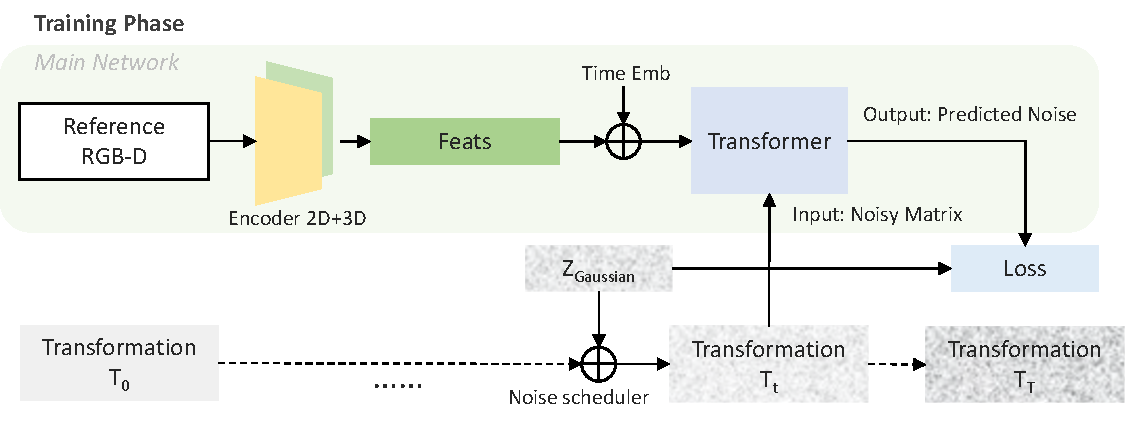
\includegraphics[width=1.0\textwidth]{img/train.pdf}
	\caption{Structure of the training phase of the pose hypotheses diffusion.}
	\label{img:train}
\end{figure}

\subsection{Sampling Phase}
Assuming that the denoiser is converged in the training phase, we can use the denoiser to iteratively generate the pose hypotheses with the randomly initialized transformation $\mathbf{T}_{T}$. Same as the training phase, we need to provide the timestep $t$ and the guidance $y$ to the backbone. Given a reference \gls{rgbd} image, we use the pre-trained \gls{2d} and \gls{3d} encoder to extract the downstream features and concatenate them as the conditional embedding of the diffusion backbone. 

Since during the training phase, the network has learned the noise distribution conditioned each timestep embedding, so the denoiser has the capability to predict the noise $\boldsymbol{\epsilon}_{\theta}$ from $t=T$ to $t=0$. Then we can use the equation \ref{eq:reverse} to get the pose hypothesis $\mathbf{T}_{t-1}$ and repeat the process until we get the final pose hypothesis $\mathbf{T}_{0}$. 

In the training phase, we feed the network with batches of data that are different in the timestep $t$ and the guidance $y$ (different reference images). During the sampling phase, we can easily make the batch size to one and only infer one pose hypothesis $\mathbf{T}_{0}$ for one reference input. Another efficient way is to simultaneously sample multiple pose hypotheses by batchifying the randomly initialized transformation and conditioning with the same reference input. The mean of the sampled pose hypotheses can be more precisely estimated as the final pose estimation if the pose of the object is uniquely determined in the space. This can be switched so that the batch of the random Gaussian initialization is conditioned with different reference inputs, which can infer multiple poses for different frames or different objects.

After the optional multi-hypotheses inference, we can further use some algorithms to refine the pose. In our model, we choose \gls{icp}\cite{121791} algorithm to refine the pose hypotheses and finally get the output transformation $\mathbf{T}_{r}$. The structure of the sampling process is shown in figure \ref{img:sample}. Details of each model in the training phase and sampling phase will be introduced in the next section.
\begin{figure}[h]
	\centering
	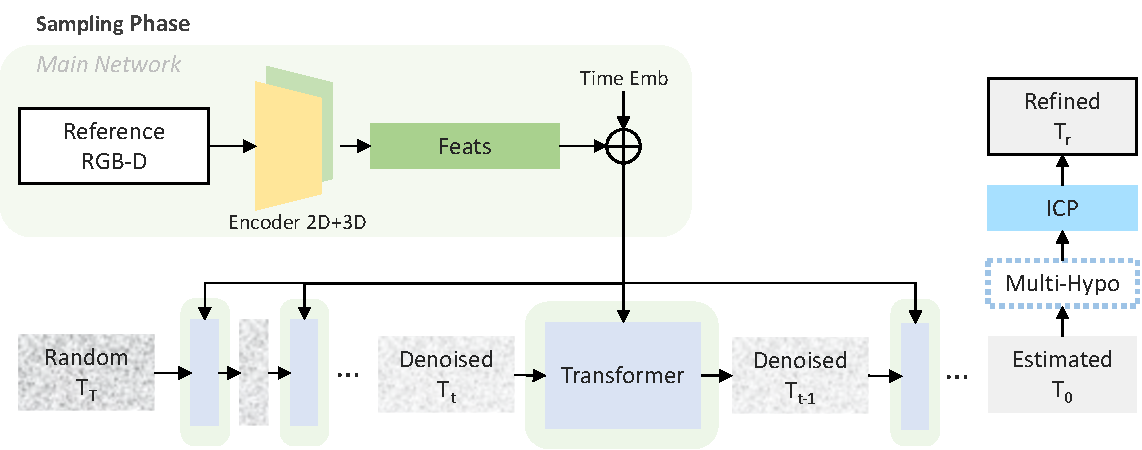
\includegraphics[width=1.0\textwidth]{img/sample.pdf}
	\caption{Structure of the sampling phase of the pose hypotheses diffusion.}
	\label{img:sample}
\end{figure}

\subsection{Speed up Sampling with DDIM}
It is relatively slow to generate the sample from \gls{ddpm} because the denoising process follows the whole Markov chain of the reverse process which is quite long. Slow inference reduced the performance of the real-time application of pose estimation, which we need to optimize. In order to speed up the sampling process, we use the \gls{ddim} \cite{song2022denoising} with the same training procedure as \gls{ddpm} but more efficient in the reverse process.

First, we rewrite the reverse conditional probability in \ref{eq:reverse_q} to be parameterized by a desired standard deviation $\sigma_{t}$ using the reparameterization trick in \ref{eq:xt_x0} as:
\begin{align}
  q_{\sigma}(\mathbf{x}_{t-1}|\mathbf{x}_{t},\mathbf{x}_{0}) = \mathcal{N} (\mathbf{x}_{t-1}; \sqrt{\bar{\alpha}_{t-1}}\mathbf{x}_{0}+\sqrt{1-\bar{\alpha}_{t-1} - \sigma_{t}^{2}}\frac{\mathbf{x}_{t}-\sqrt{\bar{\alpha}_{t}}\mathbf{x}_{0}}{\sqrt{1-\bar{\alpha}_{t}}}, \sigma_{t}^{2}\mathbf{I})
\end{align}
Compared with the original probability $q(\mathbf{x}_{t-1}|\mathbf{x}_{t},\mathbf{x}_{0}) = \mathcal{N} (\mathbf{x}_{t-1}; \boldsymbol{\tilde{\mu}}(\mathbf{x}_{t}, \mathbf{x}_{0}), \tilde{\beta}_{t}\mathbf{I})$, we have:
\begin{align}
  \tilde{\beta}_{t}=\sigma_{t}^{2}=\frac{1-\bar{\alpha}_{t-1}}{1-\bar{\alpha}_{t}}\cdot\beta_{t}
\end{align}
Then we let $\sigma_{t}^{2}=\eta\cdot\tilde{\beta}_{t}$ where $\eta$ is a hyperparemeter that controls the sampling stochasticity. $\eta=0$ corresponds the best performance of the model and $\eta=1$ corresponds to the original \gls{ddpm}. In the reverse process, we only sample a subset of the complete diffusion steps $\{\tau_{1},...\tau_{S}\}$ and the reverse process can be formulated as:
\begin{align}
  q_{\sigma,\tau}(\mathbf{x}_{\tau_{i}-1}|\mathbf{x}_{\tau_{i}},\mathbf{x}_{0}) = \mathcal{N} (\mathbf{x}_{\tau_{i}-1}; \sqrt{\bar{\alpha}_{t-1}}\mathbf{x}_{0}+\sqrt{1-\bar{\alpha}_{t-1} - \sigma_{t}^{2}}\frac{\mathbf{x}_{\tau_{i}}-\sqrt{\bar{\alpha}_{t}}\mathbf{x}_{0}}{\sqrt{1-\bar{\alpha}_{t}}}, \sigma_{t}^{2}\mathbf{I})
\end{align}
With \gls{ddim} we can use a non-Markovian diffusion process whose reverse process can be much faster than the original \gls{ddpm} and still keep the quality of the samples. It also remains the consistency of the reverse process when $\eta=0$, where the reverse process is deterministic. That makes sure that multiple samples from the same reference input have similar high-level features and in our case, the pose hypotheses are consistent with each other.
\section{Models}
\subsection{Denoiser Network}
The following figure \ref{img:denoiser} illustrates the structure of our main network in the diffusion model. As in the previous section mentioned, the transformer encoder processes the translation and rotation vector together with their position embedding conditioned with time embedding and \gls{2d}/\gls{3d} feature embedding of the reference image and predicts the noise added at this timestep. 

It is worth mentioning that the fusion of \gls{2d} and \gls{3d} feature is not pointwise aligned, which means we don't extract the pointwise feature from the \gls{2d} and \gls{3d} domain and feed to the network. Instead of doing that, we separately extract the global features and concatenate them together in order to reduce the difficulty of the convergence of the backbone with the tradeoff of the robustness and generalization of the model. This part of optimization will be discussed later.
\begin{figure}[h]
	\centering
	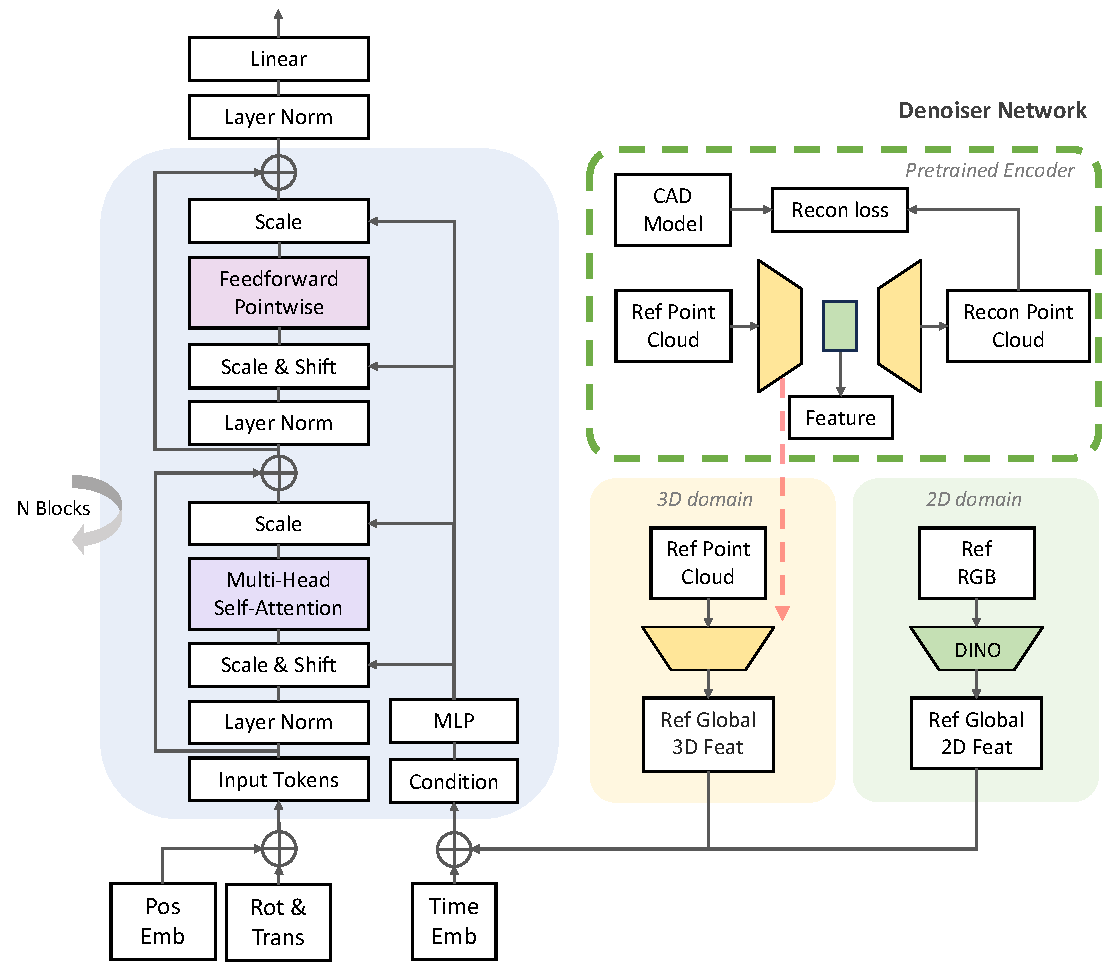
\includegraphics[width=1.0\textwidth]{img/denoiser.pdf}
	\caption{Denoiser network with backbone and feature extractor.}
	\label{img:denoiser}
\end{figure}

\subsection{Backbone}
A modified transformer encoder is utilized as the backbone of our diffusion model. The Transformer \cite{vaswani2023attention} is a sequence-to-sequence model that uses multi-head self-attention layers to understand the relevant token in the sequence and follows the encoder-decoder structure in the \gls{nlp} tasks. However, in our case, the encoder part is what we need to estimate the noise.

Similar to the vanilla transformer, our model consists of N stacked transformer encoder blocks. As shown in the left part of figure \ref{img:denoiser}, each block is made up of two sub-layers. The first is a multi-head self-attention mechanism, and the second is a simple, position-wise fully connected feed-forward network. We use residual connections around each of the two sub-layers and the \gls{ln} is applied before each sub-layer, which follows the design of \gls{vit} \cite{dosovitskiy2021image}.
\begin{figure}[h]
	\centering
	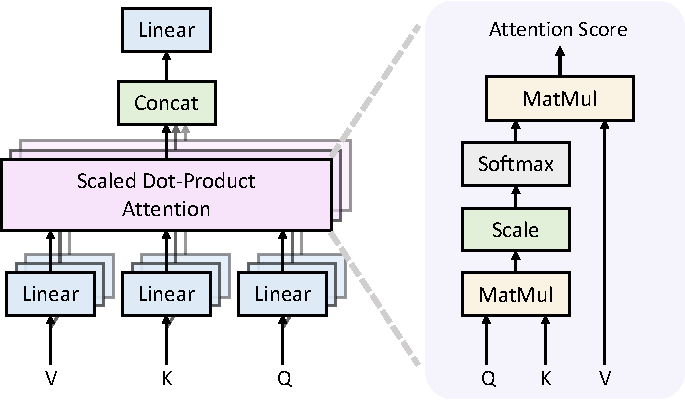
\includegraphics[width=0.7\textwidth]{img/mhsa.pdf}
	\caption{Multi-head self-attention and scaled dot-product attention.}
	\label{img:mhsa}
\end{figure}

The core of the transformer encoder is the multi-head self-attention mechanism, which is illustrated in figure \ref{img:mhsa}. First, we create three vectors from each input vector $\mathbf{x}_{i}$, namely the query vector $\mathbf{q}_{i}$, the key vector $\mathbf{k}_{i}$ and the value vector $\mathbf{v}_{i}$. These vectors are created by multiplying the input vector $\mathbf{x}_{i}$ with three matrices $\mathbf{W}^{Q}$, $\mathbf{W}^{K}$ and $\mathbf{W}^{V}$ respectively that we trained during the training phase. Then we use the scaled dot-product attention to calculate the output vector $\mathbf{y}_{i}$:
\begin{align}
  \mathbf{y}_{i} = \text{softmax}\left(\frac{\mathbf{q}_{i}\mathbf{k}_{i}^{T}}{\sqrt{d_{k}}}\right)\mathbf{v}_{i}
\end{align}
where $d_{k}$ is the dimension of the key vector $\mathbf{k}_{i}$. The scaled dot-product attention is the core of the transformer encoder and the multi-head self-attention is the extension of the scaled dot-product attention. The multi-head self-attention is defined as:
\begin{align}
  \text{MultiHead}(\mathbf{Q}, \mathbf{K}, \mathbf{V}) = \text{Concat}(\mathbf{h}_{1},...,\mathbf{h}_{n})\mathbf{W}^{O}
\end{align}
where $\mathbf{h}_{i} = \text{Attention}(\mathbf{Q}\mathbf{W}_{i}^{Q}, \mathbf{K}\mathbf{W}_{i}^{K}, \mathbf{V}\mathbf{W}_{i}^{V})$ and $\mathbf{W}_{i}^{Q}$, $\mathbf{W}_{i}^{K}$, $\mathbf{W}_{i}^{V}$ and $\mathbf{W}^{O}$ are the trainable parameters. The multi-head self-attention allows the model to jointly attend to information from different representation subspaces at different positions. With a linear projection at the end, the model is able to learn a more complex function.

To effectively process the conditional input, we use modified \gls{adaln} to replace the original layer normalization in the transformer encoder which is introduced in \cite{perez2017film,Peebles2022DiT}. The learnable scale and shift parameters are regressed from the conditional input and applied in each sub-layer of the transformer encoder blocks. The modified transformer encoder block can be formulated as:
\begin{align}
  \mathbf{y}^{'} &= \alpha_{1}(\mathbf{c})\odot {\text{Attention}[\gamma_{1}(\mathbf{c})\odot N(\mathbf{x}) + \beta_{1}(\mathbf{c})]}\\
  \mathbf{y} &= \alpha_{2}(\mathbf{c})\odot {\text{FeedForward}[\gamma_{2}(\mathbf{c})\odot N(\mathbf{y}^{'}) + \beta_{2}(\mathbf{c})]}
\end{align}
where $\mathbf{y}$ is the output of the block, $\mathbf{y}^{'}$ is the intermediate expression after the first sub-layer,  $\mathbf{c}$ is the conditional input, $\alpha_{1}(\mathbf{c})$, $\alpha_{2}(\mathbf{c})$, $\beta_{1}(\mathbf{c})$, $\beta_{2}(\mathbf{c})$, $\gamma_{1}(\mathbf{c})$ and $\gamma_{1}(\mathbf{c})$ are the learnable parameters and $N$ is the layer normalization. The $\odot$ denotes the element-wise multiplication.

\subsection{Time Embedding and Postion Embedding}
Why do we need time embedding and position embedding in our case? The architecture of the diffusion model determines that we need to let the network learn the influence of timestep on the noise estimation. So we have to encode the timestep information into the network. For the same reason, the sequence of the transformer input which is the transformation vector is also relevant and should be encoded, because each bit of the vector represents a different meaning and can not be shuffled.

The way we embed time and position information is generally called positional encoding. It should satisfy the following conditions \cite{kazemnejad2019:pencoding}:
\begin{itemize}
  \item It should be unique and deterministic defined for each position (or timestep).
  \item The encoded distance between any two steps should be consistent across different timesteps.
  \item The value should be bounded and generalized to any input.
\end{itemize}
The most common positional encoding is the sine and cosine positional encoding \cite{vaswani2023attention}, which is defined as:
\begin{align}
  \text{PE}_{(pos, 2i)} &= \sin\left(\frac{pos}{10000^{2i/d_{model}}}\right)\\
  \text{PE}_{(pos, 2i+1)} &= \cos\left(\frac{pos}{10000^{2i/d_{model}}}\right)
\end{align}
where $pos$ is the position, $i$ is the dimension and $d_{model}$ is the dimension of the input vector. And we add a fully connected layer to the positional encoding to make it trainable. Figure \ref{img:pe} shows the 64-dimensional positional encoding for a sequence with a length of 100 using the sine and cosine positional encoding.
\begin{figure}[h]
	\centering
	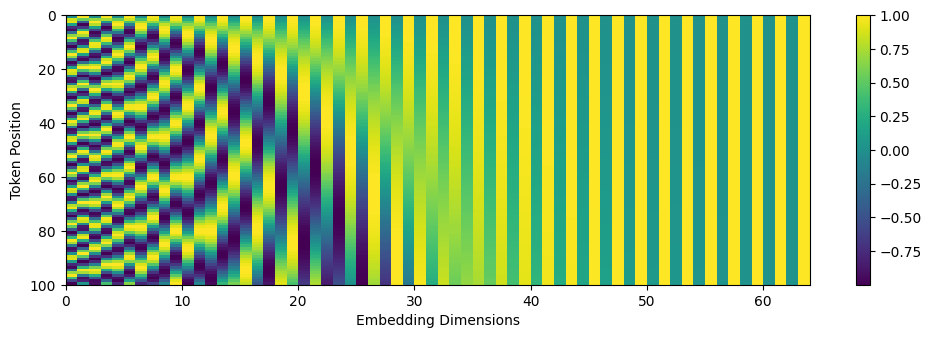
\includegraphics[width=1.0\textwidth]{img/pe.png}
	\caption{The 64-dimensional positional encoding for a sequence with a length of 100.}
	\label{img:pe}
\end{figure}

\subsection{2D Feature Extractor}
As the \gls{2d} feature extractor, the self-supervised Vision Transformer
 with DINO \cite{caron2021emerging} is used. DINO is a self-supervised learning method that trains a Vision Transformer
 with a small set of negative examples. It is a contrastive learning method that maximizes the agreement between differently augmented views of the same image. The architecture of DINO shares the same overall structure with recent self-supervised approaches and also similarities with knowledge distillation.

Knowledge distillation is a learning paradigm where a student network $g_{\theta_{s}}$ is trained to match the output of a given teacher network $g_{\theta_{t}}$, parameterized by $\theta_{s}$ and $\theta_{t}$ respectively. Given an input image $x$, both networks output probability distributions over $K$ dimensions denoted by $P_{s}$ and $P_{t}$. The probability $P$ is obtained by normalizing the output of the network $g$ with a softmax function. Given a fixed teacher network $g_{\theta_{t}}$, the student network $g_{\theta_{s}}$ is trained to minimize the cross-entropy loss between the two distributions w.r.t the student parameters $\theta_{s}$:
\begin{align}
  L = \mathop{min}_{\theta_{s}}H(P_{t}(x), P_{s}(x))
\end{align}
where $H(a,b)=-a \log b$ is the cross-entropy loss. This optimization problem is adapted to self-supervised learning by constructing different distorted views or crops of an image with a multi-crop strategy. Making a set of two global views, $x_{1}^{g}$ and $x_{2}^{g}$ and several local views with smaller resolution, the loss function can be formulated as:
\begin{align}
  L_{DINO}=\mathop{min}_{\theta_{s}}\mathop{\sum}_{x\in \{x_{1}^{g},x_{2}^{g}\}} \ \mathop{\sum}_{x^{'}\in V \atop x^{'}\neq x}H(P_{t}(x), P_{s}(x^{'}))
\end{align}
The structure of the self-supervised architecture is shown in figure \ref{img:dino}. The model passes two different random transformations of the input image to both networks with the same structure but different parameters. The output of the teacher network is centered and a \gls{sg} is applied on the teacher to let the gradients only propagate through the student network. The teacher parameters are updated with an \gls{ema}.
\begin{figure}[h]
	\centering
	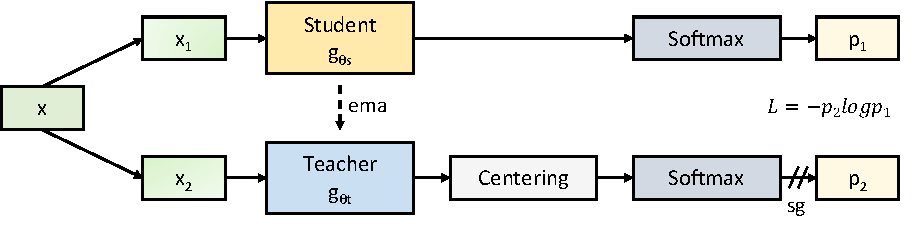
\includegraphics[width=0.85\textwidth]{img/dino.pdf}
	\caption{Self-supervised architecture of DINO.}
	\label{img:dino}
\end{figure}

The backbone of the DINO is \gls{vit} \cite{dosovitskiy2021image}, which proved that the transformer architecture also performs well on the \gls{2d} vision tasks. The standard transformer processes \gls{1d} sequences, and in order to handle \gls{2d} images, the input is first flattened into a sequence of patches. For a input image $x\in R^{H\times W\times C}$ and patch size $p$, the patchified input can be denoted as $x_p\in R^{N\times(p^{2}C)}$ with the number of patches $N=HW/{p^{2}}$. The reason why the patches are fed into the transformer rather than the raw image is that it is relatively easier for the network to understand the relationship between the patches than the raw pixels.

Similar to the vanilla transformer for \gls{nlp} tasks, the patches need to be embedded with the positional encoding. A standard learnable \gls{1d} position embedding is used in the original paper. In order to solve the classification task with \gls{vit}, an extra token is added to the sequence of patches, which is called the class token. An additional \gls{mlp} layer is used for the classification. But for the downstream tasks like ours, we only need the latent feature from the transformer encoder output. The overview of the \gls{vit} model is shown in figure \ref{img:vit}, using the illustration in the original publication.
\begin{figure}[h]
	\centering
	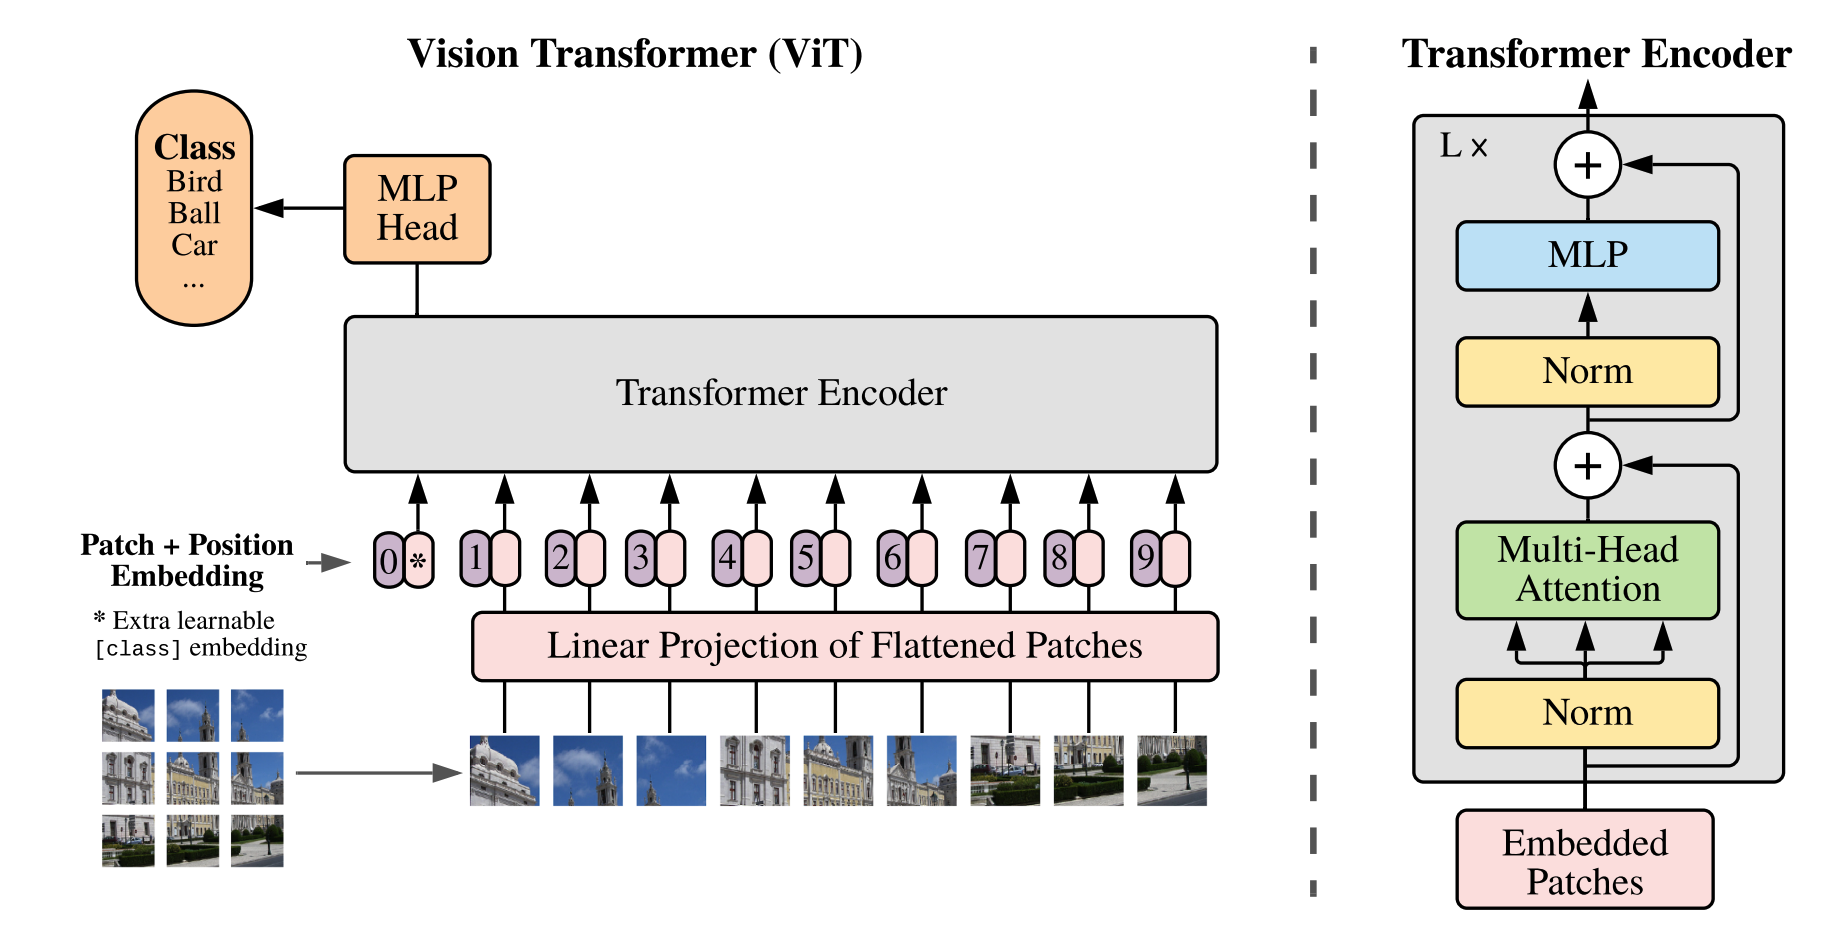
\includegraphics[width=1.0\textwidth]{img/vit.png}
	\caption{Sturcture of the ViT model, image adapted from the original paper \cite{dosovitskiy2021image}.}
	\label{img:vit}
\end{figure}

Compared with the convolutional neural network which has a dominant position in the field of \gls{2d} vision tasks, the Vision Transformer has advantages as well as drawbacks under some scenarios. The transformer is more computationally expensive and requires more memory than the convolutional neural network. And the transformer is not as robust as the convolutional neural network in the case of a small dataset. On the other hand, Vision Transformer architecture is more flexible and can be easily applied to different tasks with different input sizes. It offers a more natural way to process the \gls{2d} image, which is more similar to the human brain. The transformer is more suitable for tasks that require the global information of the image, such as the classification task. In our case, we use the Vision Transformer pre-trained with DINO to extract the global feature of the reference image and feed it to the transformer encoder as the conditional embedding.

We directly use the weights of the model pre-trained on ImageNet \cite{5206848}, because the \gls{2d} feature downstream network generalizes well on other datasets than \gls{3d} feature extractor, which has right now rare well generalized downstream backbones that can cover any \gls{3d} objects. For this reason, we train the \gls{3d} feature extractor from scratch on the dataset we use and this part will be introduced in the next section.

\subsection{3D Feature Extractor}
Due to the permutation invariance and transformation invariance of the point cloud, the \gls{3d} networks are differently constructed compared with the \gls{2d} networks. Famous works like PointNet \cite{qi2017pointnet} and PointNet++ \cite{qi2017pointnet++} are the pioneers of the \gls{3d} deep learning. After that, the convolutional neural network is also introduced to the \gls{3d} domain such as KPConv \cite{thomas2019kpconv}. 

In our case, we use an encoder-decoder architecture to first build up a point cloud completion task of the target dataset and utilize the latent feature from the encoder output as the \gls{3d} global feature of the reference \gls{rgbd} image. The reason for using the point cloud completion task rather than the classification or semantic segmentation task is that we need the network to learn the geometrical features such as shape, position and orientation of the object. The point cloud completion is more suitable than separately reconstructing the \gls{cad} model and reference partial point cloud because the network can learn the relationship between the two point clouds and the latent feature is more robust and generalizable.
\begin{figure}[h]
	\centering
	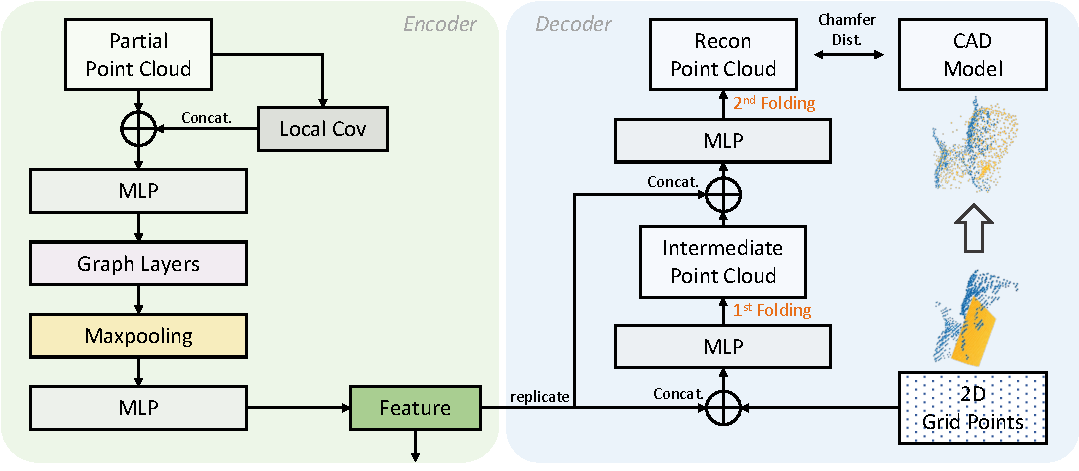
\includegraphics[width=1.0\textwidth]{img/fold.pdf}
	\caption{3D feature extraction with FoldingNet-based point cloud completion.}
	\label{img:fold}
\end{figure}

FoldingNet consists of a graph-based encoder and a folding-based decoder. The graph-based encoder follows the design of \cite{shen2018mining} using the graph structure of the point cloud neighborhood. The encoder is built up with \gls{mlp} and graph-based max-pooling layers, which are constructed from the k-nearest neighbor through the spatial position of the nodes in the point cloud. For each point, a local covariance matrix with the size of 3x3 is computed, flattened to a vector and concatenated with the point position as the input vector fed to the network. Afterward, the input vector is passed through \gls{mlp} and graph layers to get the topology information of the local neighborhood. Then the max-pooling is applied to all nodes and the global feature is projected to a latent space by using another perceptron.

The folding-based decoder is built up with two consecutive \gls{mlp} to wrap a fixed \gls{2d} grid into the shape of the reference point cloud and that explains why this network is called FoldingNet. First, a \gls{2d} grid matrix is initialized in a standard square shape at the origin and is concatenated with the replicated latent feature from the encoder output to become the input of the first folding \gls{mlp}. The output is the first folded point cloud and it is again concatenated with the replicated latent feature and fed to the second folding \gls{mlp}.

The final output point cloud is aligned with the reference point cloud using the bi-directional \gls{cd} as the loss function, which can be formulated as:
\begin{align}\label{eq:cd}
  L_{CD}(S, \hat{S}) = \max \left\{\frac{1}{\lvert S\rvert }\mathop{\sum}_{x\in S} \mathop{\min}_{\hat{x}\in \hat{S}}||x-\hat{x}||_{2} ,\ \frac{1}{\lvert \hat{S}\rvert }\mathop{\sum}_{\hat{x}\in \hat{S}} \mathop{\min}_{x\in S}||\hat{x}-x||_{2}\right\}
\end{align}
where $S$ is the reference point cloud and $\hat{S}$ is the output point cloud. The formulation enforces that the output point cloud is close to the reference point cloud and vice versa. In our case, given a partial point cloud as input, the reconstructed point cloud is aligned with the \gls{cad} model at the pose of the partial point cloud. The structure of the FoldingNet is shown in figure \ref{img:fold}.

\subsection{Feature Fusion}\label{sec:fusion}
The way of fusing the features and embedding from different domains determines the performance of the model and the convergence of the training phase. Because features may compensate each other or may be redundant in some cases and the network cannot efficiently learn the relationship between the latent feature and the ground truth. In our model, we have the following feature or embedding vectors that need to be integrated into the network: the \gls{2d} feature $f_{2D}$ from the pre-trained DINO model, the \gls{3d} feature $f_{3D}$ from the pre-trained FoldingNet model, the positional encoding of the timestep (time embedding) $e_{t}$ and the positional encoding of the transformation vector (position embedding) $e_{p}$.

For the position embedding $e_{p}$, we follow the pipeline of the Transformer that $e_{p}$ is directly added to the input vector $x_{t}$ which is first replicated to the dimension of the hidden dimension of the network. For the conditional guidance of the diffusion model $f_{2D}$, $f_{3D}$ and $e_{p}$, we have two ways introduced in our setup to merge these features into the backbone. The first method is that these features are projected separately to the hidden dimension of the network with fully connected layers and then added together. Another way is to directly concatenate these features along the feature dimension and then project them to the hidden dimension. After that, the merged feature vector is fed to the Transformer encoder with \gls{adaln} after each attention layer and feed-forward layer. Figure \ref{img:fuse} illustrates the detail of the feature fusion process using both methods.
\begin{figure}[h]
  \centering
  \subfloat[]{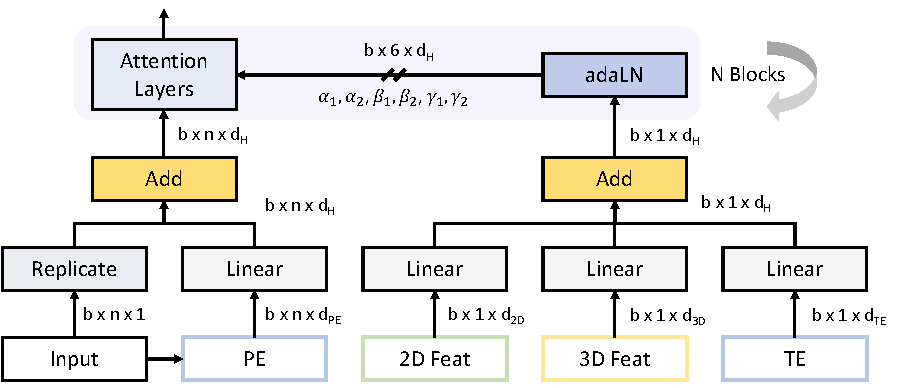
\includegraphics[width=0.95\textwidth]{img/fuse_add.pdf} } \\
  \centering
  \subfloat[]{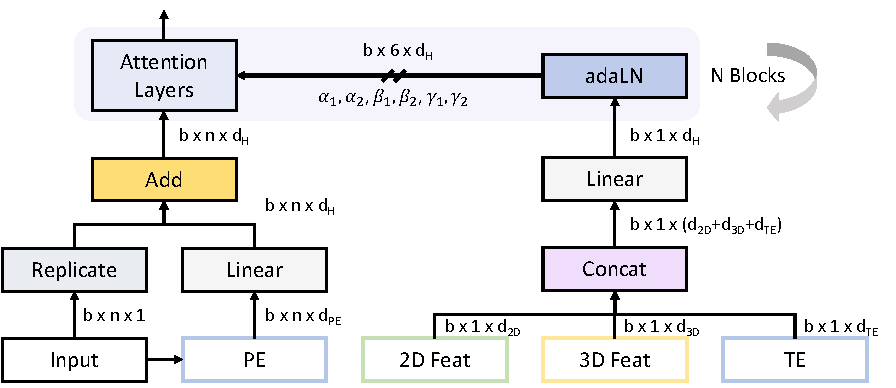
\includegraphics[width=0.95\textwidth]{img/fuse_cat.pdf} } 
  \caption{Structure of the feature fusion process using (a): addition of the conditional features and embedding; (b): concatenation of the conditional features and embedding.}
  \label{img:fuse}
\end{figure}


\subsection{Residual Translation}\label{sec:res_t}
Compared with the rotation estimation in the \gls{6dof} estimation task, translation is relatively easier to determine, at least in a rough range. We can use the position of the bounding box of the object in the camera coordinate combined with the camera parameter to calculate the coarse position of the object in the \gls{3d} space. In another way, we can directly use the mean of the point cloud's position to roughly approximate the translation if the depth information is available. The error exists mainly because the point cloud is sometimes not complete so the gravity center of the partial point cloud is not the real center of the object. That's also the reason for the error of the \gls{2d} only method that the occlusion causes a shift between the center of the visible part and the ground truth.

With the help of the deep learning method, we can minimize the error of the estimation when we use the gravity center of the reference point cloud as the initial translation. The model is trained to learn the residual translation from the gravity center to the ground truth center. First, we calculate the mean of the reference point cloud ($\overrightarrow{OQ}$ in figure \ref{img:res_t}) which is the initial translation and move the point cloud to the origin. Then we let the network minimize the residual error between the estimated translation and the shifted ground truth translation $\overrightarrow{OP^{'}}$. The estimated residual translation is added to the initial translation $\overrightarrow{OQ}$ to get the final translation estimation $\overrightarrow{OP} $. This process basically enables the network to approximate the shift between the mean of the partial point cloud and its original center, instead of the position of the object in the \gls{3d} space. This modification reduces the solving space significantly compared with directly estimating the translation $\overrightarrow{OP} $ and makes the training more efficient.

\begin{figure}[h]
	\centering
	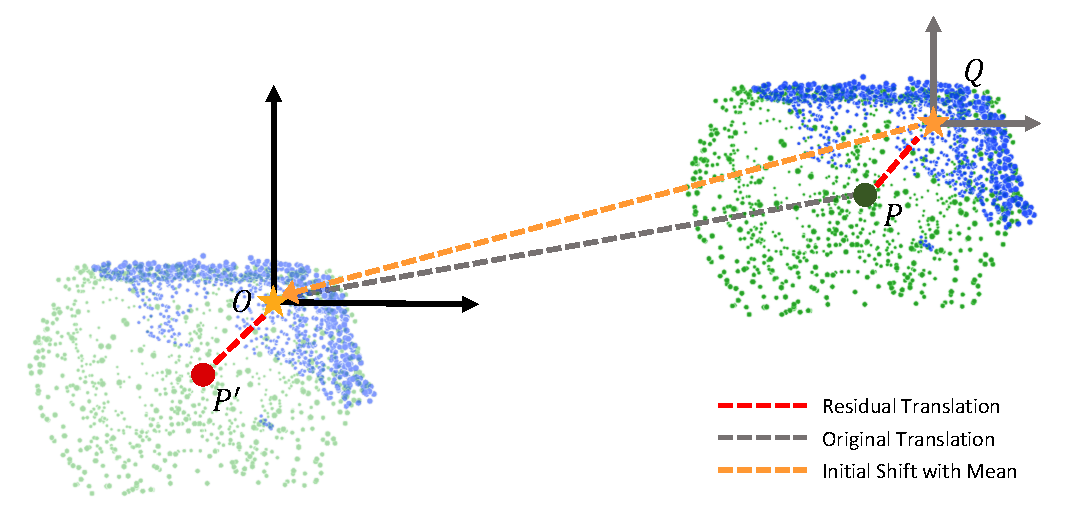
\includegraphics[width=0.8\textwidth]{img/res_t.pdf}
	\caption{Illustration of the residual translation estimation (projected in 2D space).}
	\label{img:res_t}
\end{figure}

\subsection{Multi-Hypotheses Inference}
One of the advantages of the diffusion model is the high quality and diversity of the generated objects. Using the case of image synthesis as an example, we can derive dozens of high-resolution and meaningful images from the diffusion model with the same prompt. In our case, we want to first use the multi-hypotheses module to reduce the variance of the generated poses by taking the mean of all hypotheses as the final estimation and making the final result more robust. In the feature work, we may sample more hypotheses to analyze the pose distribution of symmetrical objects in order to explore more possibilities when we deal with the ambiguity of the pose estimation.

\subsection{Pose Refinement}
To further refine the \gls{6dof} pose of the reference input, we can use the coarse pose estimation from the diffusion model as the initial pose and use some algorithms to refine the pose. Iterative and not learning-based methods like \gls{ransac} \cite{10.1145/358669.358692} and \gls{icp} \cite{121791} are popular in the field of pose estimation. \gls{ransac}, for example, uses repeated random sub-sampling to iteratively estimate the optimal result in the set of data containing outliers. The goal of \gls{ransac} is to find a global optimal solution that excludes the outliers and contains the inliers as much as possible. This technique is widely used in correspondence-based point cloud registration. Our pose hypotheses diffusion model samples directly the estimated \gls{6dof} pose of the reference input and we utilize \gls{icp} to the point cloud transformed via the coarse pose estimation. 

The \gls{icp} algorithm is also an iterative solution to the rigid point cloud registration problem. Given a set of source points $A$ and a set of target points $B$, the goal of \gls{icp} is to find a rigid transformation $(\mathbf{R},\mathbf{t})$ that minimizes the distance between the source points and the transformed target points. The first step is to find the corresponding points pair using nearest neighbor search. Let the set of corresponding pairs be:
\begin{align}
  C = \{(i,j)\ \vert \ \mathbf{a}_{i}\in A \ \text{and} \ \mathbf{b}_{j}\in B \ \text{are corresponding points}\}
\end{align}
After that, we use the sum of the squared distance of the corresponding point pairs as the error to be minimized. The minimization problem can be formulated as:
\begin{align}
  (\mathbf{R}^{*}, \mathbf{t}^{*})=\mathop{argmin}_{\mathbf{R},\mathbf{t}}\sum_{(i,j)\in C}||\mathbf{Ra}_{i}+\mathbf{t}-\mathbf{b}_{j}||_{2}^{2}
\end{align}
To solve this problem efficiently, we normally use the \gls{svd} which guarantees the accuracy and speed during a large number of iterations. The \gls{icp} algorithm is summarized in the following algorithm \ref{algo:icp}:
\begin{algorithm}[ht]
  \caption{Iterative Closest Point}
  \label{algo:icp}
  \begin{algorithmic}[1]
    \Require
      Source point cloud $A=\{\mathbf{a}_{i}\}_{i=1}^{N}$, target point cloud $B=\{\mathbf{b}_{i}\}_{i=1}^{N}$, maximum number of iterations $k_{max}$, threshold $\epsilon$
    \Ensure
      Rigid transformation $(\mathbf{R},\mathbf{t})$
    \State Initialize $(\mathbf{R},\mathbf{t})$ with coarse pose estimation
    \For{$k=1$ to $k_{max}$}
      \State $A^{*}\longleftarrow \text{Trans}(A, (\mathbf{R},\mathbf{t}))$
      \State $C=\{(i,j)\ \vert \ \mathbf{a}_{i}\in A \ \text{and} \ \mathbf{b}_{j}\in B \}\longleftarrow \text{NearstSearch}(A^{*}, B)$
      \State $(\mathbf{R}, \mathbf{t})\longleftarrow \text{SVD}(C)$
      \State $e = \frac{1}{\lvert C\rvert}\sum_{(i,j)\in C}||\mathbf{Ra}_{i}+\mathbf{t}-\mathbf{b}_{j}||_{2}^{2}$
      
      \If{$e<\epsilon$}
        \State Break
      \EndIf
    \EndFor
  \end{algorithmic}
\end{algorithm}

\begin{figure}[h]
  \centering
  
\includegraphics[width=0.9\textwidth]{img/spacer.pdf}
  \label{img:spacer}
\end{figure}

Theoretically, the \gls{icp} algorithm can converge to the global optimal solution if the initial pose is close enough to the ground truth pose. However, in practice, the \gls{icp} algorithm is sensitive to the initial pose and can easily get stuck in the local optimal solution. Because of that, we use the coarse pose estimation from the diffusion model as the initial pose and run the \gls{icp} algorithm within an acceptable number of iterations to have a good tradeoff of inference speed and accuracy. 

\chapter{Experiments}
In this section, we first introduce the datasets we use in our experiments and then we show the details of the training and evaluation of the pose hypotheses diffusion model and its feature extractors on the datasets. We compare our model with other methods and show the ablation study of our model.
\section{Datasets}
\subsection{LINEMOD Dataset}
The \gls{lm} dataset \cite{hinterstoisser2012model} is a widely used dataset for the \gls{6dof} pose estimation. It has 15 objects containing ape, bench vise, bowl, camera, can, cat, cup, driller, duck, egg box, glue, hole puncher, iron, lamp and phone. These objects are texture-less with discriminative color, shape and size and are placed in a cluttered scene. As the training dataset, it provides for each object 1312 \gls{rgbd} images from different viewpoints annotated with the ground truth. These training data are based on the synthetic \gls{cad} Model without any occlusion and noise. There are also vividly rendered training data placed together in the scene to simulate the real scenario. The \gls{bop} \cite{hodan2018bop} introduced the training data generated from an open-source, light-weight, procedural and photorealistic \gls{pbr} renderer BlenderProc \cite{denninger2019blenderproc} into the \gls{lm} dataset.
This set of \gls{pbr}-BlenderProc4BOP training images are sorted in 50 different scenes with 50000 images in total which are rendered with different lighting, and occlusion. The test datasets are captured with the Kinect sensor. The following figures \ref{img:linemod} show the training data and test data of the \gls{lm} dataset.
\begin{figure}[h]
  \centering
  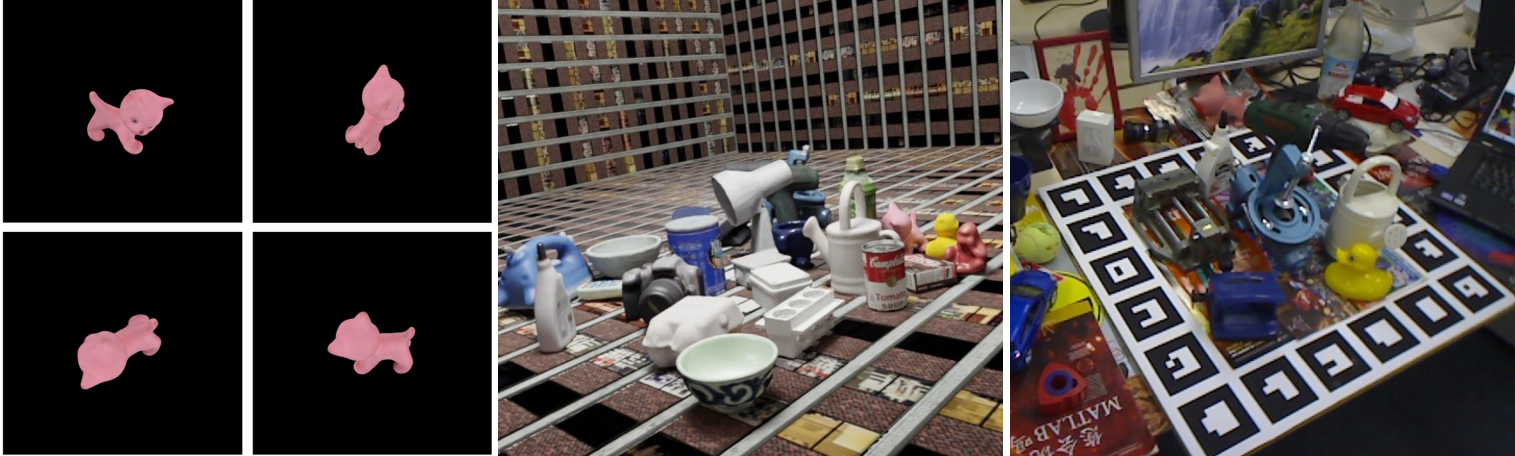
\includegraphics[width=1.0\textwidth]{img/lm.pdf}
  \caption{LIMEMOD dataset. Left: training data with Synthetic CAD Model; Middle: training data rendered with PBR-BlenderProc4BOP; Right: test data captured with Kinect Sensor.}
  \label{img:linemod}
\end{figure}

\subsection{LINEMOD-O Dataset}
To evaluate the model on the occluded scene, Brachmann et al. \cite{dataV4MUMX2020} refined the bench-vise partition of the \gls{lm} dataset with occluded objects and annotated ground truth pose under different light conditions to make the pose estimation more challenging. The meaning of the high-level occlusion data is to simulate the real scenario where the object is partially occluded by other objects so that the model can learn the robustness of the pose estimation and generalize better to the real-world data. The following figure \ref{img:linemod_o} shows the low-level occluded scene and high-level occluded scene.
\begin{figure}[h]
  \centering
  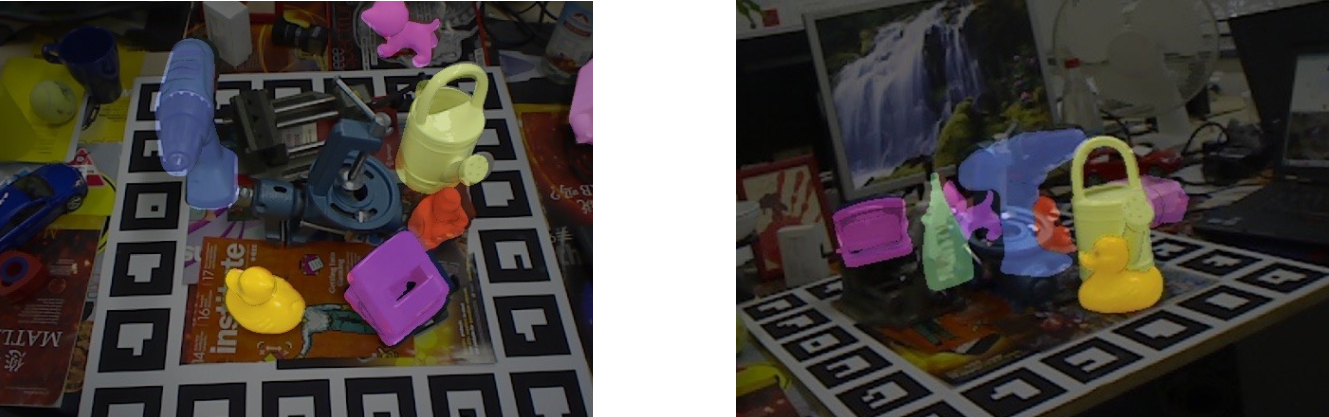
\includegraphics[width=0.9\textwidth]{img/lmo.pdf}
  \caption{Comparison of LMO dataset with LM dataset. Left: low-level occluded scene; Right: high-level occluded scene.}
  \label{img:linemod_o}
\end{figure}
\subsection{Data Format}
In order to unify the data format of the different datasets for \gls{6dof} pose estimation task. We follow the data format of the \gls{bop} dataset. The structure of the dataset is shown in the following table \ref{tab:dataset}.
\begin{table}[ht]
  \centering
  \caption{Dataset Structure of BOP Format.}
  \label{tab:dataset}
  \begin{tabular}{l l}
      \toprule
      Directory & Contents \\
      \midrule
      DATASET\_NAME & \\
      |--- camera[\_TYPE].json & Camera parameters\\
      |--- dataset\_info.json & Dataset-specific information\\
      |--- test\_targets\_bop19.json & Test targets for the BOP Challenge \\
      |--- models[\_MODELTYPE][\_eval] & \\
      | \quad |--- models\_info.json & Dimension and symmetry\\
      | \quad |--- obj\_OBJ\_ID.ply & \gls{3d} file of the object\\
      |--- train|val|test[\_TYPE] & Training/Validation/Test images\\
      | \quad |--- SCENE\_ID|OBJ\_ID & \\
      | \quad | \quad |--- scene\_camera.json & Camera parameters of the scene\\
      | \quad | \quad |--- scene\_gt.json & Ground truth annotation\\
      | \quad | \quad |--- scene\_gt\_info.json & Meta information\\
      | \quad | \quad |--- depth & Depth images\\
      | \quad | \quad |--- mask & Masks of object silhouettes\\
      | \quad | \quad |--- mask\_visib & Masks of the visible parts of object silhouettes\\
      | \quad | \quad |--- rgb|gray & Color/gray images\\
      \bottomrule
  \end{tabular}
\end{table}

Clarification of the naming in table \ref{tab:dataset}:
\begin{itemize}
  \item models[\_MODELTYPE]\_eval: "Uniformly" resampled and decimated \gls{3d} object models used for calculation of errors of object pose estimates.
  \item MODELTYPE, TRAINTYPE, VALTYPE and TESTTYPE are optional and used if more data types are available (e.g. images from different sensors).
\end{itemize}
Camera parameters in scene\_camera.json:
\begin{itemize}
  \item cam\_K - 3x3 intrinsic camera matrix K (saved row-wise).
  \item depth\_scale - Multiply the depth image with this factor to get depth in mm.
  \item cam\_R\_w2c (optional) - 3x3 rotation matrix R\_w2c (saved row-wise).
  \item cam\_t\_w2c (optional) - 3x1 translation vector t\_w2c.
  \item view\_level (optional) - Viewpoint subdivision level.
\end{itemize}
Ground truth annotation in scene\_gt.json:
\begin{itemize}
  \item obj\_id - Object ID.
  \item cam\_R\_m2c - 3x3 rotation matrix R\_m2c (saved row-wise).
  \item cam\_t\_m2c - 3x1 translation vector t\_m2c.
\end{itemize}
Meta information of the ground truth in scene\_gt\_info.json:
\begin{itemize}
  \item bbox\_obj - \gls{2d} bounding box of the object silhouette given by (x, y, width, height), where (x, y) is the top-left corner of the bounding box.
  \item bbox\_visib - \gls{2d} bounding box of the visible part of the object silhouette.
  \item px\_count\_all - Number of pixels in the object silhouette.
  \item px\_count\_valid - Number of pixels in the object silhouette with valid depth.
  \item px\_count\_visib - Number of pixels in the visible part of the object silhouette.
  \item isib\_fract - The visible fraction of the object silhouette.
\end{itemize}

\subsection{Data Augmentation}
Although the quantity of the training data from the BlenderProc is large enough, we still need some data augmentation tricks to make the model more robust against noise and invalid data. The data augmentation for the point cloud in our case is firstly the random rotation of the partial point cloud and \gls{cad} model with the modification of the ground truth transformation. We add noise to points with a Gaussian distribution scaled by a factor $k_{n}$ related to the scale of the objects to simulate the real-world data captured by the depth sensor. The symmetry of the object is also considered, and we generate extra data by flipping or rotating the symmetrical \gls{cad} models with the corresponding ground truth. 

To remove the noise and outliers in the point cloud. We use the statistical outlier filter in the data preprocessing stage. The statistical outlier filter is an algorithm that removes outliers from a point cloud based on the statistical analysis of point neighborhoods. The algorithm removes points that are further away from their neighbors compared to the average for the point cloud. The filter is controlled by the number of neighbors $n_{nb}$ and the standard deviation multiplier $\sigma$.

After that, the point cloud is then downsampled to 1000 points to reduce the computational cost but still maintain the geometry information of the object. The whole original training dataset is divided into the training part (90\%) and validation part (10\%) randomly and together with the separate test dataset we get the dataset we preprocessed for the training and evaluation of our models.

As the \gls{2d} image is combined with \gls{3d} point cloud in the pose estimation task and we don't need to train the \gls{2d} feature extractor, we only use the data augmentation of the random rotation during the training of the \gls{3d} feature extractor. Because the \gls{2d} image with \gls{3d} depth uniquely defines uniquely the \gls{6dof} pose of the object. So during the training of the pose estimation task we don't let orginal point cloud rotate, but still add noise and consider the symmetry of the object.
\section{Implementation Details}
In this section, we first present the implementation of the \gls{2d} and \gls{3d} feature extractors and the corresponding evaluations on the module level. Then we demonstrate the training details of our diffusion model.
\subsection{2D Feature Extractor}
\subsubsection{Pretrained Model} 
DINO, as our \gls{2d} feature encoder, provides many pre-trained weights of the backbone with different numbers of parameters and backbone architecture which are pre-trained on ImageNet for general image downstream tasks. The evaluation of the self-supervised architecture uses the linear and \gls{knn} classifier on the feature extracted from the model. The following table \ref{tab:dino} shows the evaluation results of the different pre-trained backbones on the ImageNet dataset according to the original paper \cite{caron2021emerging}.
\begin{table}[ht]
  \centering
  \caption{Evaluation of the pre-trained DINO model on ImageNet.}
  \label{tab:dino}
  \begin{tabular}{l | c c c c c c c}
      \toprule
      Backbone & \#Params. & Dim. & \#Layers & \#Heads & Patch Size & $k$-NN & Linear\\
      \midrule
      ViT-S/16 & 21M & 384 & 12 & 6 & 16 & 74.5 & 77.0 \\
      ViT-S/8 & 21M & 384 & 12 & 6 & 8 & 78.3 & 79.7 \\
      ViT-B/16 & 85M & 768 & 12 & 12 & 16 & 76.1 & 78.2 \\
      ViT-B/8 & 85M & 768 & 12 & 12 & 8 & 77.4 & 80.1 \\
      \bottomrule
  \end{tabular}
\end{table}

After we register the pre-trained \gls{2d} backbone to our model, we need to feed the image with some preprocessing into the \gls{vit}. The image is first cropped to a bounding box with the object we want to estimate its pose. Then we resize the cropped image to the size of 224x224 and normalize the image with the mean and standard deviation of the ImageNet dataset, while the \gls{vit} is pre-trained on the ImageNet. The mean and standard deviation of the \gls{rgb} channels are $(0.485, 0.456, 0.406)$ and $(0.229, 0.224, 0.225)$ respectively. After that, the image is processed following the \gls{vit} architecture and as output, we get the feature we can use in the pose estimation task. 

The \gls{2d} encoder needs to be lightweight since it is just a downstream task for our diffusion model, so in our setup we don't use the backbone with a very deep network and a large number of parameters, e.g.,\gls{vit}-L or \gls{vit}-G. It needs also to be well generalized because the image in our case is not seen during the training of the \gls{2d} encoder. ImageNet used in DINO contains more than 1.4 million annotated images from different categories, which has the capability to let the network learn the latent feature expression from the majority of real-life objects. 

\subsubsection{Evaluation}
Since we use the \gls{2d} feature not for the classification or segmentation tasks, but as the input for the pose estimation where the feature is the latent expression of pose that is hard to quantitatively evaluate, we evaluate the influence of the \gls{2d} feature extractor together with the pose estimation diffusion model later. Instead, the attention map of the input image can be visualized to indirectly evaluate the network and validate whether the Transformer can grasp the important part of the image. The attention map is the output of the last attention layer in the Transformer encoder. Figure \ref{img:atten} shows the attention maps of 3 objects as examples fed to the \gls{vit}.

\begin{figure}[h]
  \centering
  \subfloat{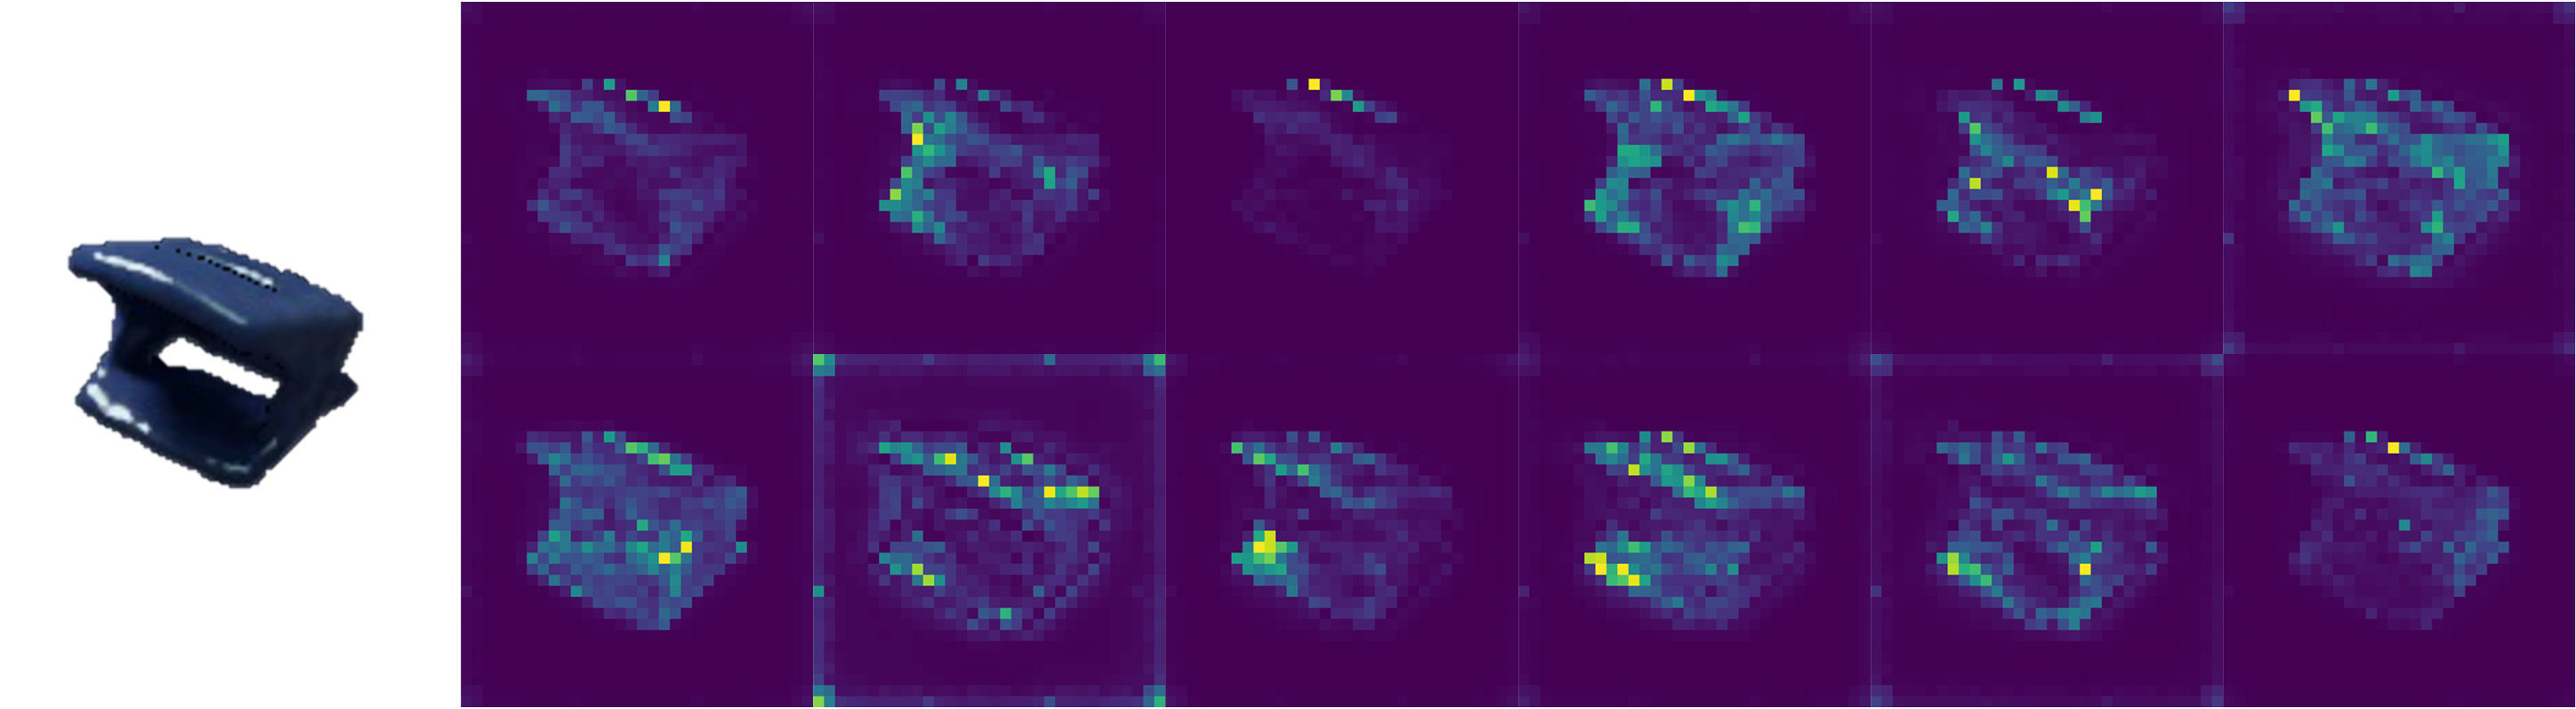
\includegraphics[width=0.98\textwidth]{img/atten_cl.png} } \\
  \centering
  \subfloat{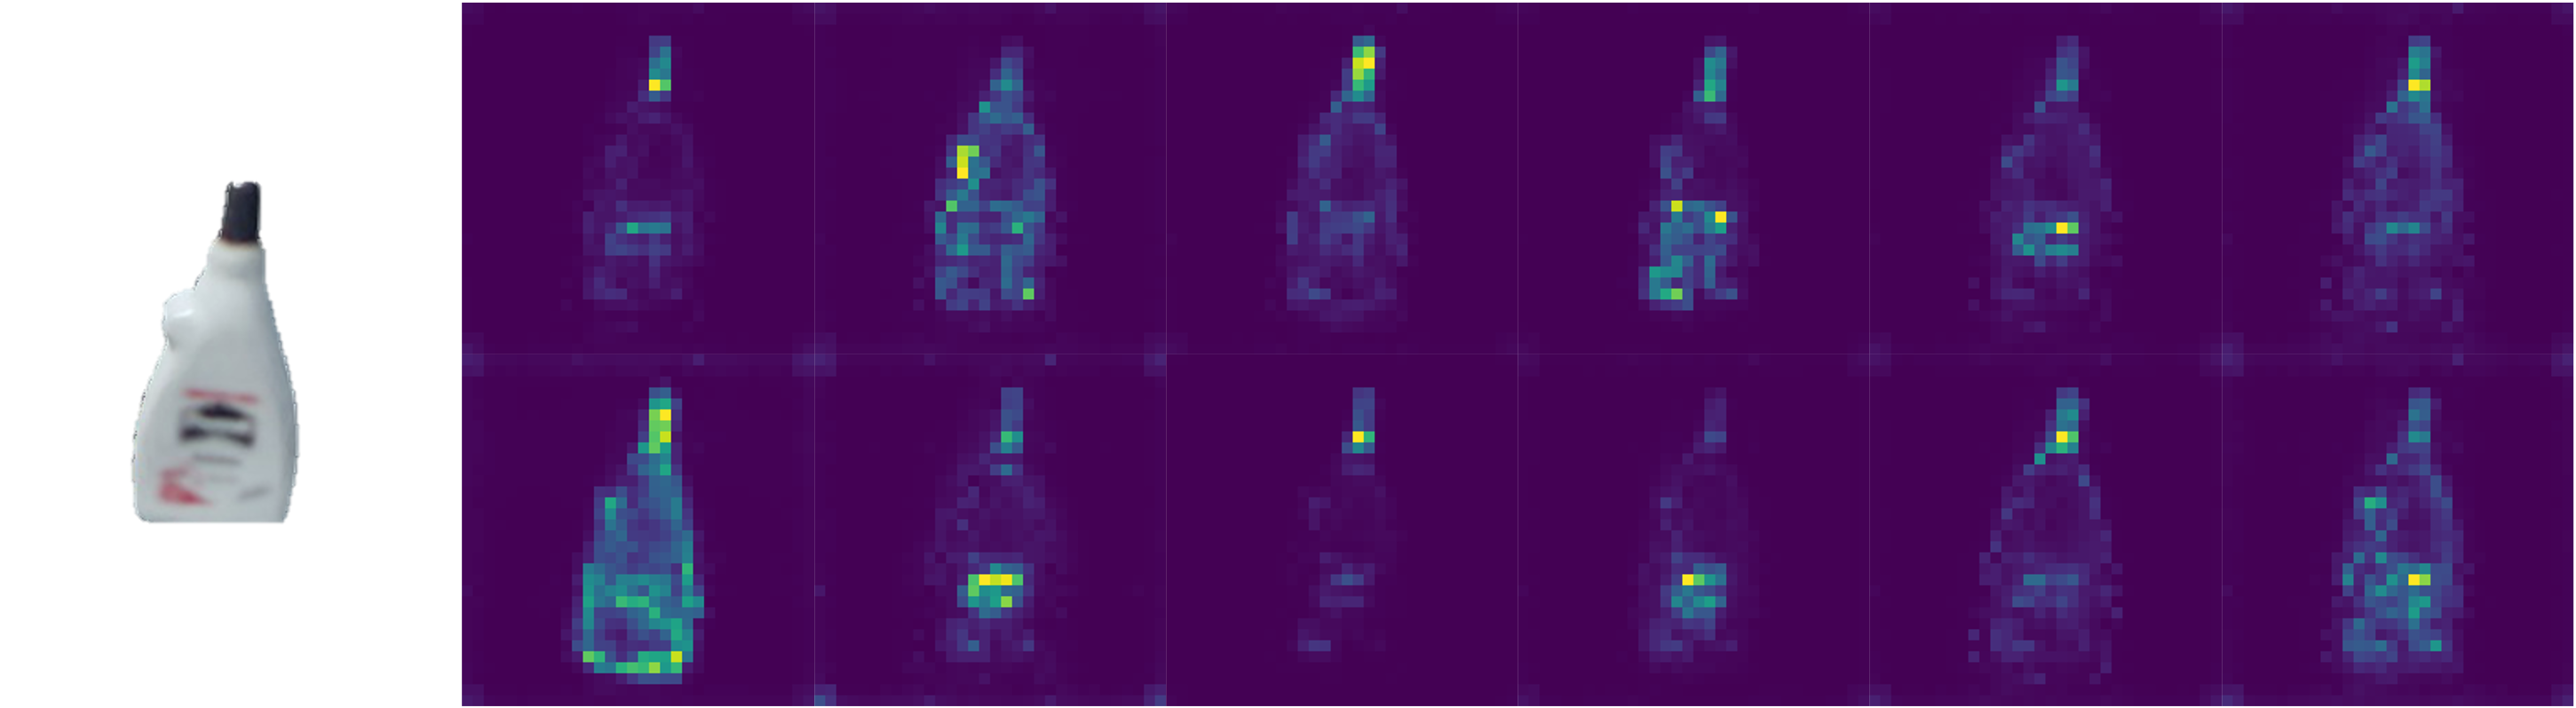
\includegraphics[width=0.98\textwidth]{img/atten_bo.png} } \\
  \centering
  \subfloat{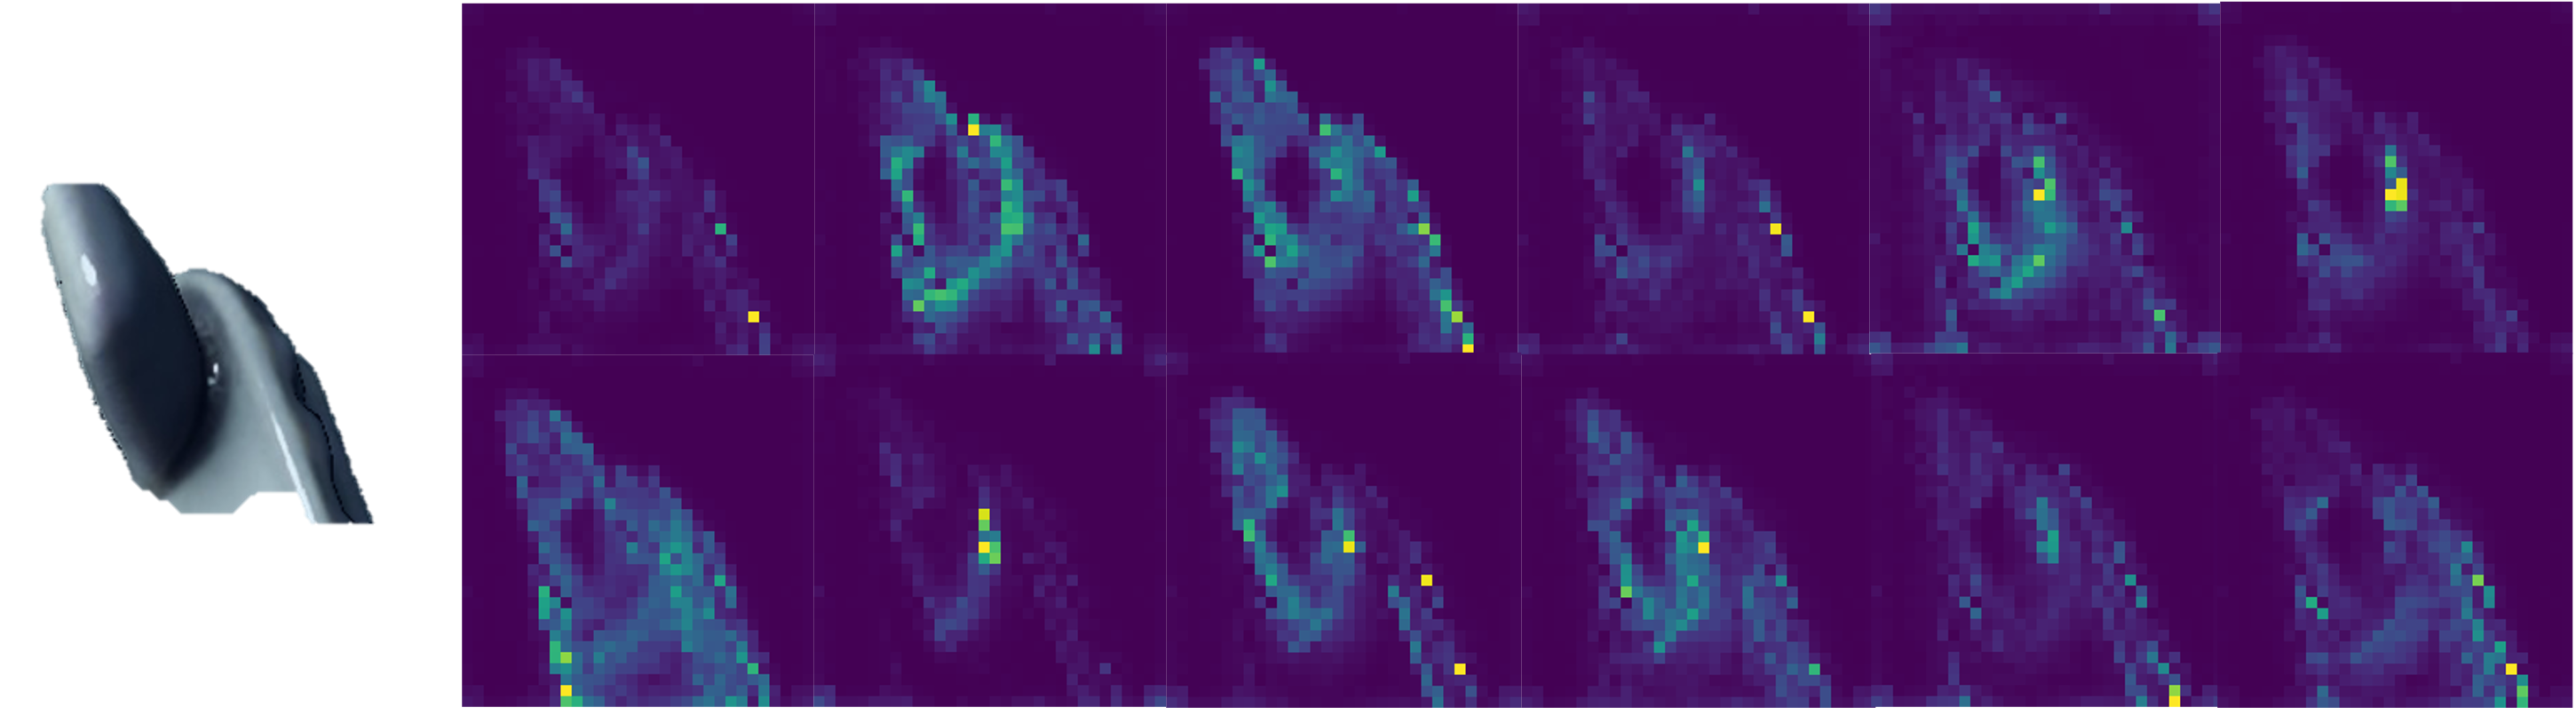
\includegraphics[width=0.98\textwidth]{img/atten_ph.png} } 
  \caption{Visualization of the attention maps of the input image, where 12 heatmaps represent 12 attention heads output in the Transformer. Top: hole puncher; Middle: glue; Bottom: phone (occluded).}
  \label{img:atten}
\end{figure}

By Comparing the outputs from a different scale of \gls{vit} models and patch size, we can find that the patch size significantly determines the attention map. Because the object we dealing with has relatively simple geometry and some sometimes textureless, the transformer can not encode the image in a very accurate way for the pose difference if the patch size is too big. The following figure \ref{img:atten_patch} shows the attention maps of the same image fed to the \gls{vit} with different patch sizes and scales of \glspl{vit}. 
\begin{figure}[h]
	\centering
	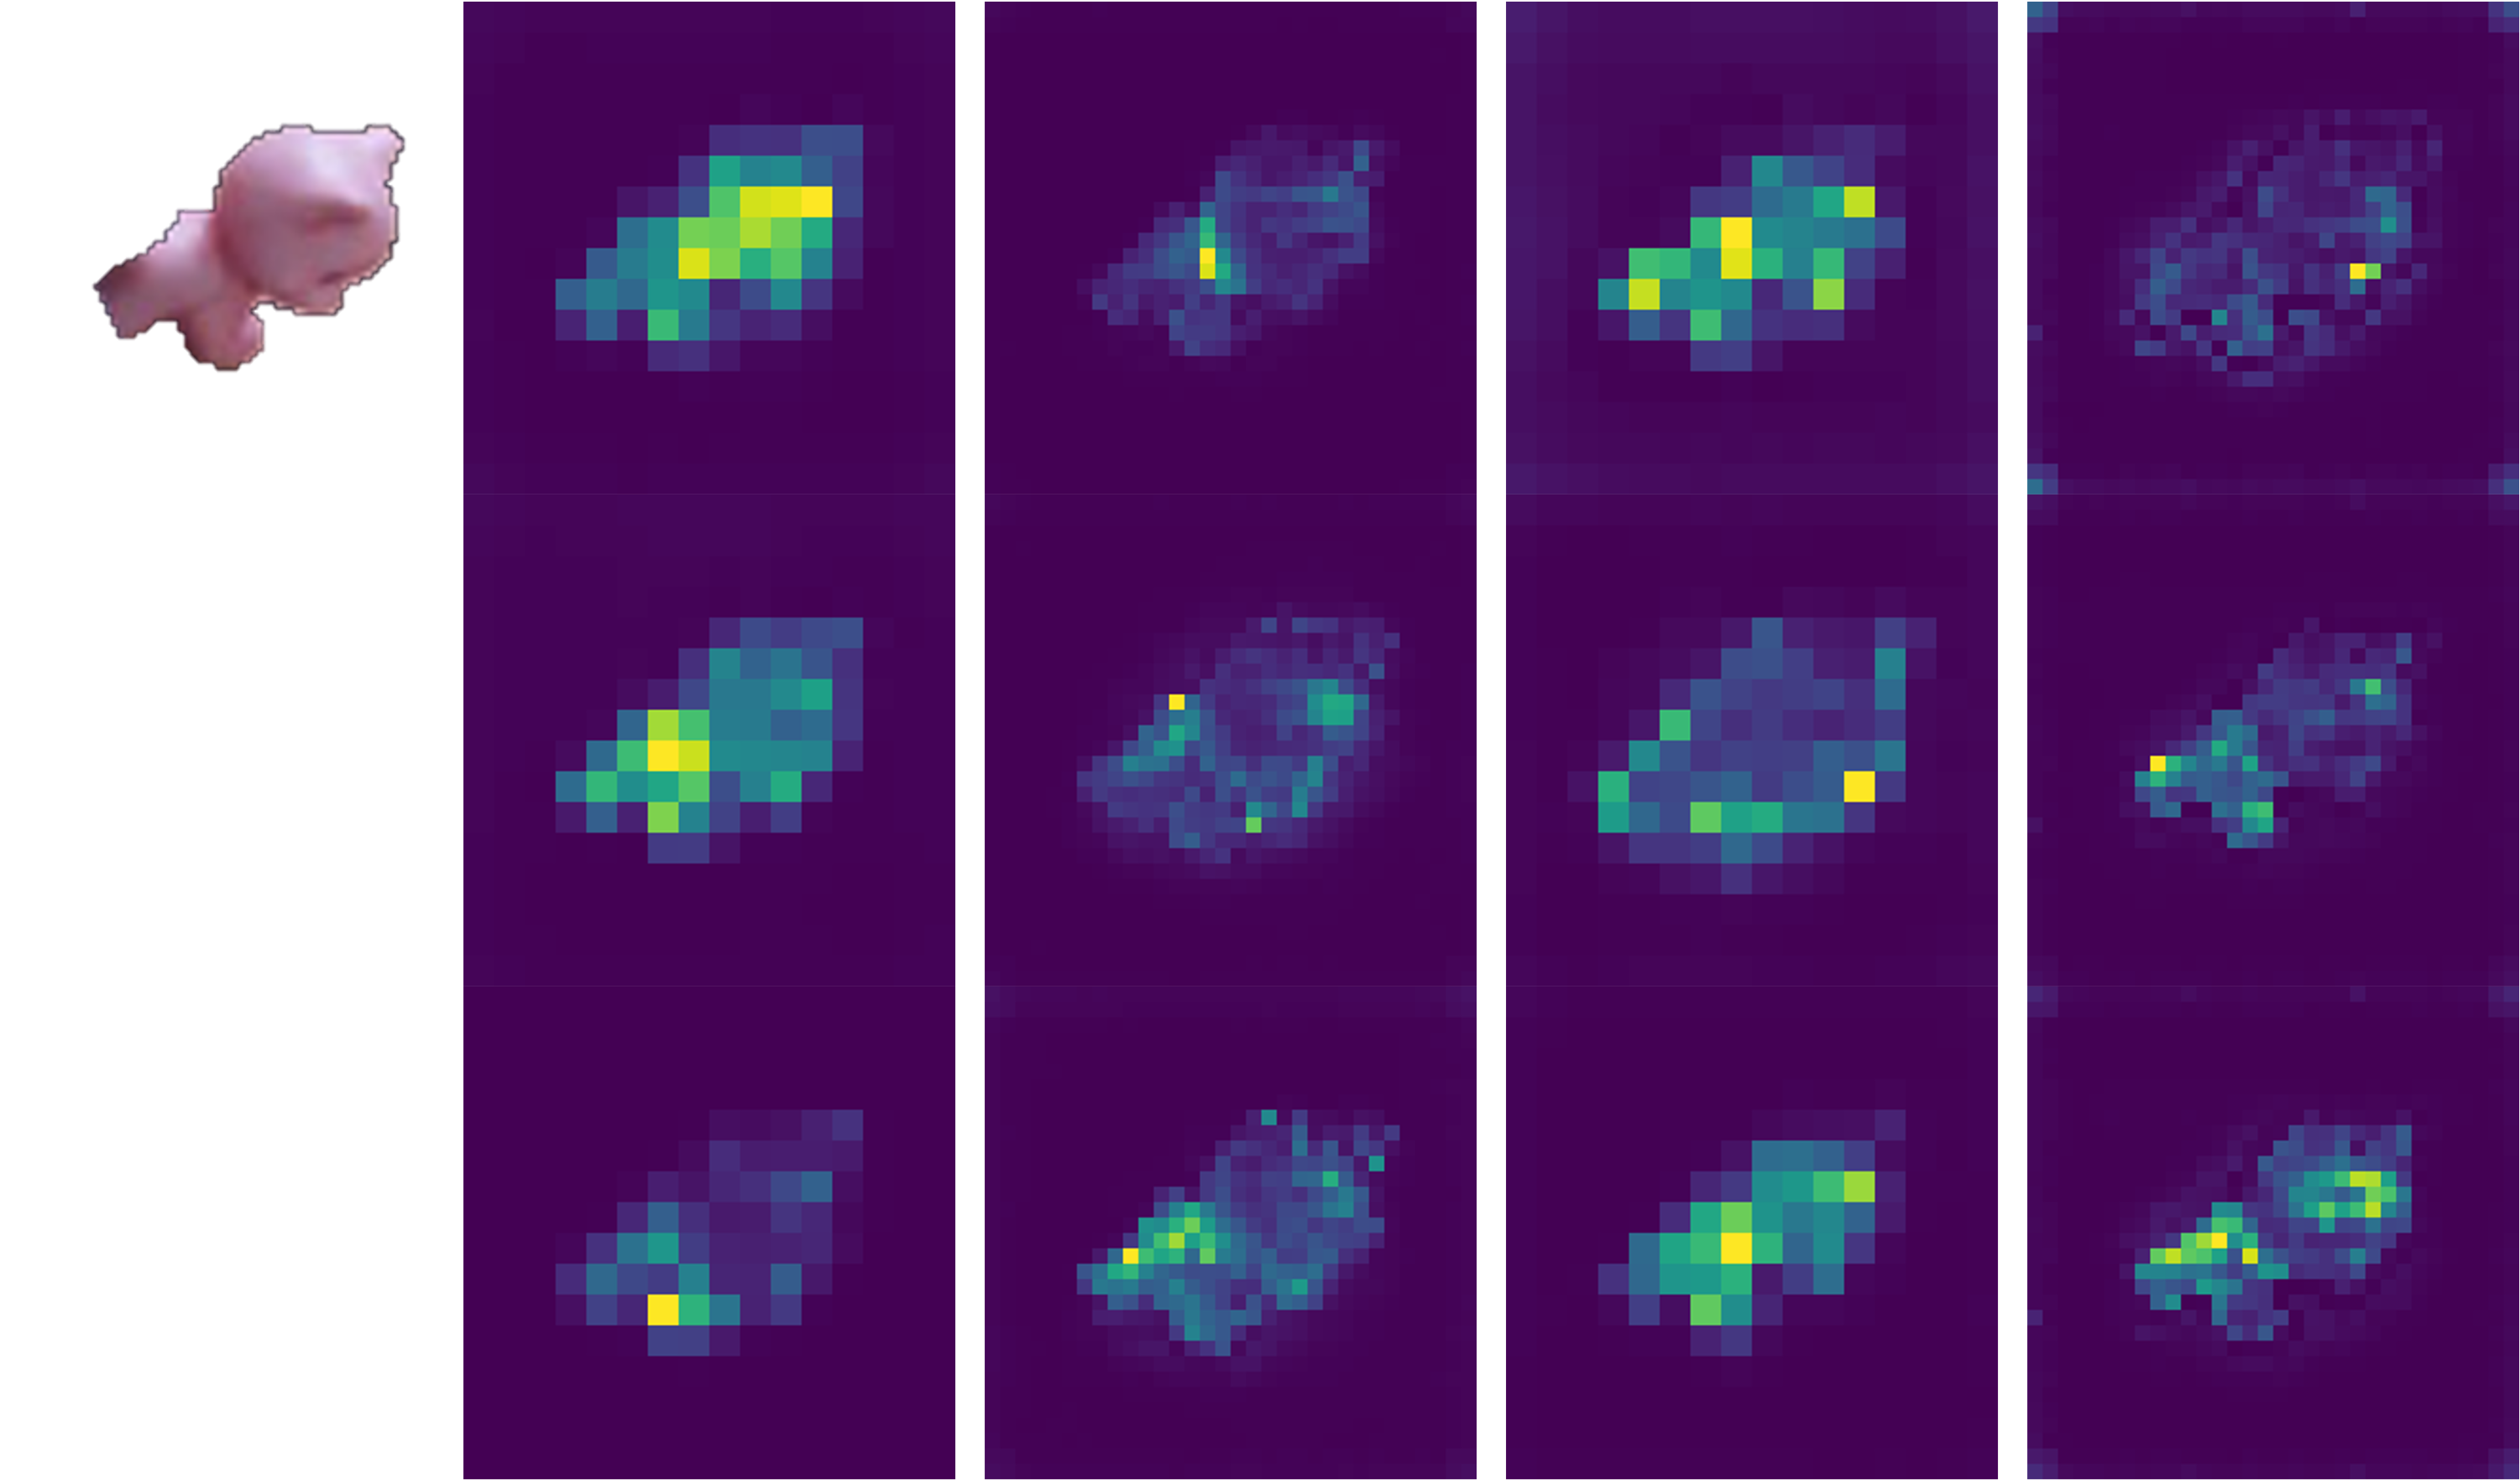
\includegraphics[width=1.\textwidth]{img/atten_cat.png}
	\caption{Attension maps of the different scales of ViTs and patch size. From left to right: ViT-S/16, ViT-S/8, ViT-B/16, ViT-B/8. Each column represents 3 random attention heads.}
	\label{img:atten_patch}
\end{figure}

From the figure \ref{img:atten_patch} we can see that the key points of the cat e.g., ears, tail and eyes are not precisely localized if the patch size is not small enough. For the classification task is this drawback not that obvious because the network can learn the latent feature from the majority of the image. But for the pose estimation task, the network needs to learn the latent feature from the key points or edges of the object, which is more sensitive to the resolution.

Considering the tradeoff of the inference speed and performance, we use \gls{vit}-B/8 in our experiments which has a quite satisfied performance and a relatively acceptable number of parameters. The ablation study of different setups will be shown later in this experiments section.

\subsection{3D Feature Extractor}
\subsubsection{Training} 
The \gls{3d} feature extractor is trained using a point cloud completion task. The reference partial point cloud is fed to the FoldingNet and the output is aligned with the \gls{cad} model transformed with the ground truth pose as the previous figure \ref{img:fold} shows. The loss function is the bi-directional \gls{cd} between the output point cloud and the transformed \gls{cad} model (see equation \ref{eq:cd}).

The model is trained on a single Nvidia Tesla V100-SXM2 video card with 16GB memory. We use the BlenderProc4BOP training dataset for LM which contains 50k images with 15 objects and we can further crop several objects from each image. To that end, we finally have more than 560k separate partial point clouds for training. After the tuning of the hyperparameters, we use the batch size of 32 and the \gls{adam} optimizer with the cosine annealing learning rate scheduler. The initial learning rate is $1e^{-4}$ and the end-up \gls{lr} is $1e^{-6}$. The model-specific hyperparameter is the number of the folding \gls{mlp} layers, which is by default set to 2 in our case. The number of \gls{knn} is set to 64 and the number of the graph-based local maxpooling layers is set to 2. The reconstructed point number is set to 2025, whose square root is an integer responding to the size of the \gls{2d} grid. The dimension of the latent feature is set to 512 for the downstream task. The model is trained for 200k iteration which is about 114 epochs.
\subsubsection{Evaluation} 
The evaluation metric of the point cloud completion task is the \gls{cd} between the output point cloud and the ground truth point cloud. The following graph \ref{img:fold_loss} shows the training and validation loss of the model during the whole training process. 

\begin{figure}[h]
	\centering
	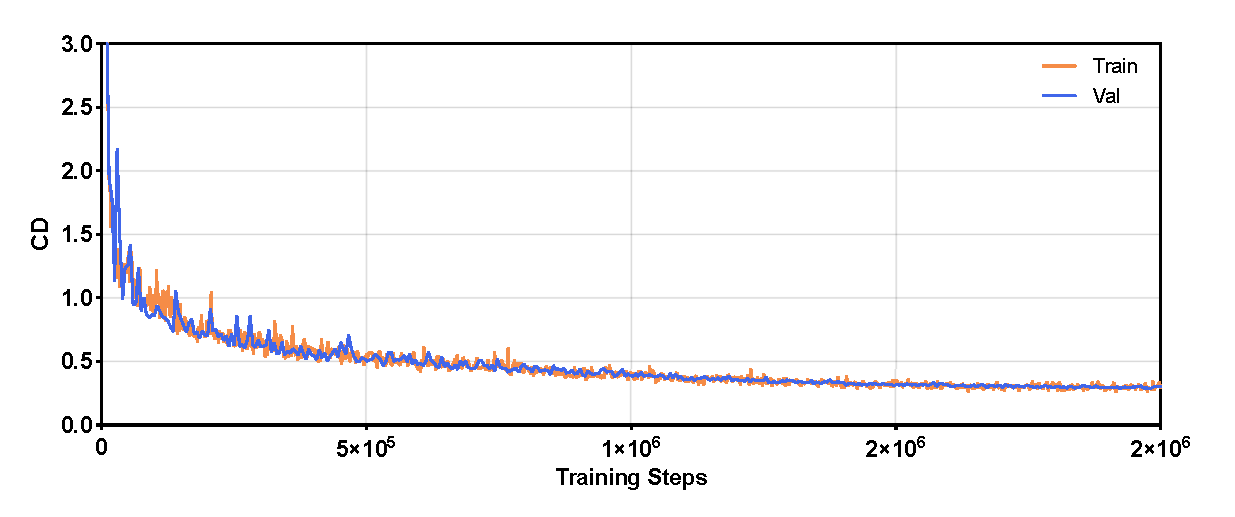
\includegraphics[width=1.\textwidth]{img/fold_loss.eps}
	\caption{CD of the training and validation dataset during the point completion pretraining.}
	\label{img:fold_loss}
\end{figure}

We stop the training after 200k iterations to prevent the overfitting problem, because the validation loss is not decreasing anymore. And the distribution of each category's \gls{cd} in the test dataset is shown in figure \ref{img:cd_cate}.

\begin{figure}[h]
	\centering
	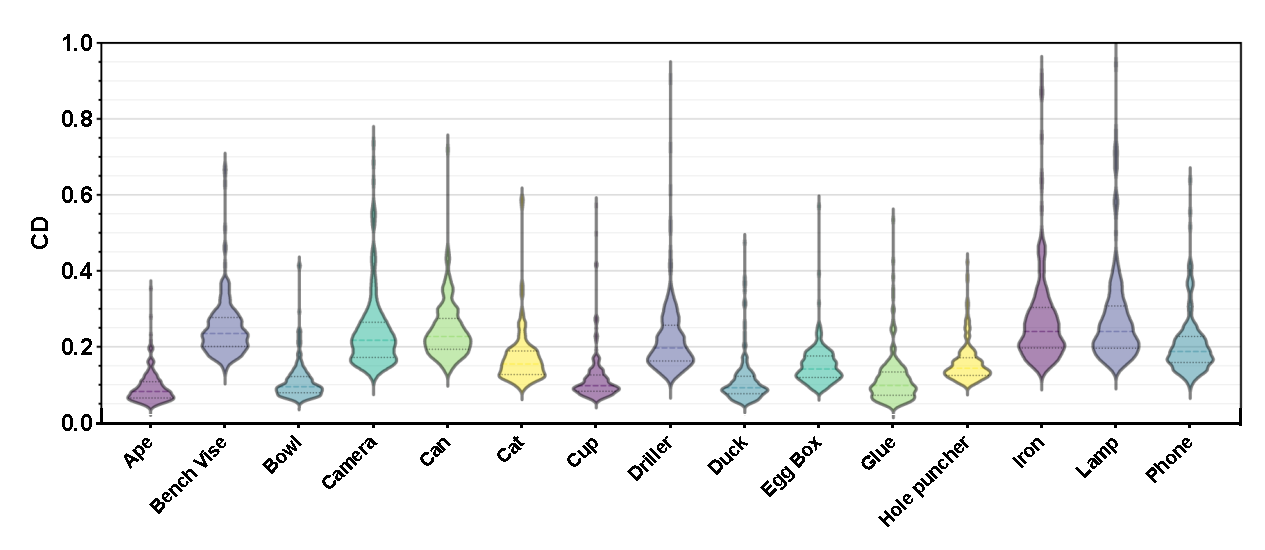
\includegraphics[width=1.\textwidth]{img/cd_category.eps}
	\caption{Categorical level CD distance distribution of the test dataset.}
	\label{img:cd_cate}
\end{figure}



With the visualization of the reconstructed point cloud (figure \ref{img:comp_all}), we can validate that the model has the capability to localize the partial point cloud and complete the missing part of the object. The implicit expression of the \gls{6dof} poses as well as the object class is learned by the model without giving the class label so that we can use the feature to represent the pose and object class of the reference input in the diffusion model.

\begin{figure}[h]
	\centering
	\subfloat{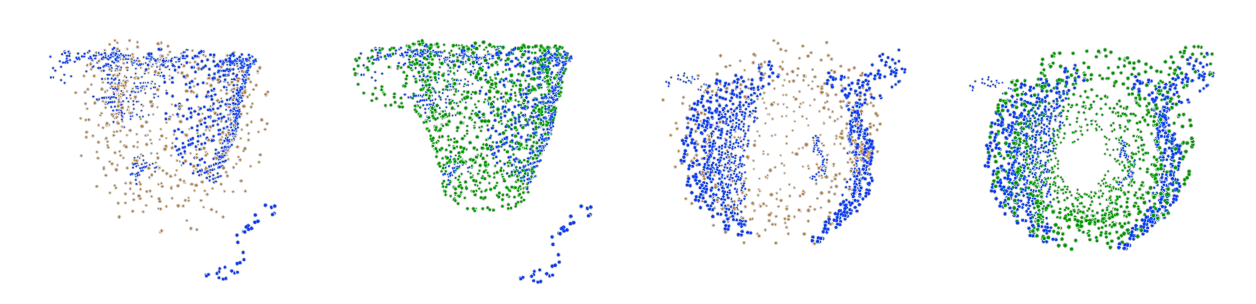
\includegraphics[width=1.\textwidth]{img/comp_cup.pdf}}\\
  \centering
	\subfloat{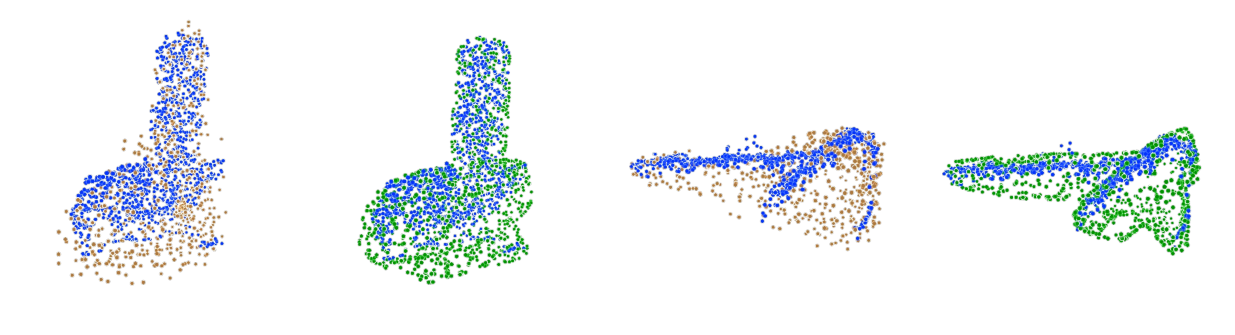
\includegraphics[width=1.\textwidth]{img/comp_phone.pdf}}
	\caption{Point cloud completion results of the FoldingNet. Top: cup; Bottom: phone. From left to right: estimation(viewpoint 1), ground truth(viewpoint 1), estimation(viewpoint 2), ground truth(viewpoint 2). Blue points are the input partial point cloud.}
	\label{img:comp_all}
\end{figure}

The following figure \ref{img:fold_dev} shows the development of the output from the FoldingNet decoder during the training process.

\begin{figure}[h]
	\centering
	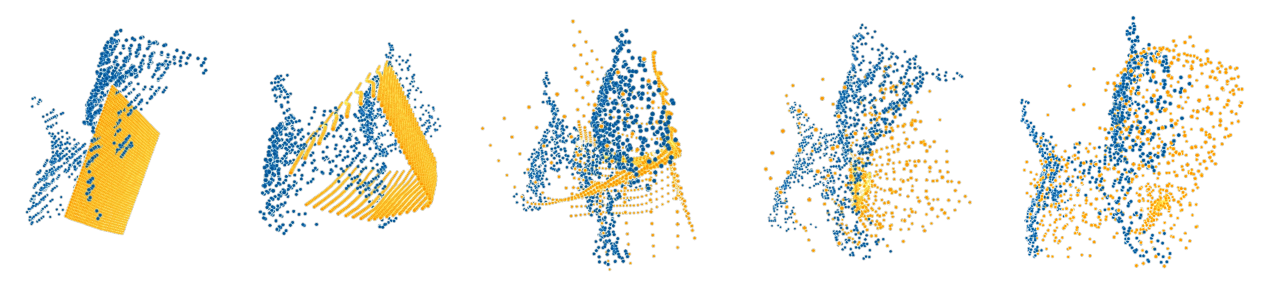
\includegraphics[width=1.\textwidth]{img/fold_dev.pdf}
	\caption{Development of the reconstructed point cloud during the training process.}
	\label{img:fold_dev}
\end{figure}

From the visualization, we can find that the shape of the reconstructed point cloud is getting more and more similar to the ground truth, but the difference exists because of the capability of the backbone on data with heavy occlusion and noise. We further compare the training of point cloud completion tasks on all 15 categories with overfitted models on a single object to validate the generalization of the network. From figure \ref{img:fold_overfit} we can find that the \gls{cd} of the overfitted models has a lower mean and variance than the model trained on all categories. Table \ref{tab:fold_overfit} shows the quantitative comparison.
\begin{figure}[h]
	\centering
	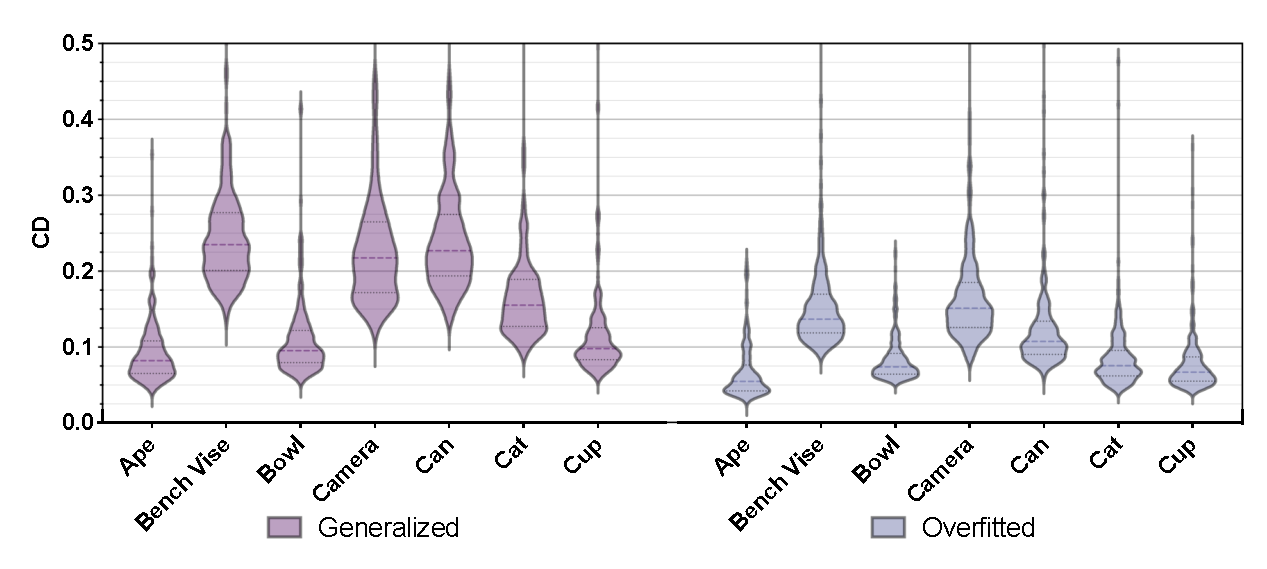
\includegraphics[width=1.\textwidth]{img/fold_overfit.eps}
	\caption{Comparision of the CD distributions between the model trained with the whole data set and the overfitted model on a single object (the first 7 objects of LM are shown).}
	\label{img:fold_overfit}
\end{figure}

\begin{table}[h]
  \centering
  \caption{Mean and standard deviation of the CD with the model trained on the whole dataset and the overfitted model on a single object (7 of 15 objects selected).}
  \label{tab:fold_overfit}
  \begin{tabular}{l | C{12mm} C{12mm} C{12mm} C{12mm} C{12mm} C{12mm} C{12mm} | C{12mm}}
      \toprule
      \multicolumn{9}{c}{Trained on the complete LM} \\
      \midrule
      Category & Ape & Vise & Bowl & Cam. & Can & Cat & Cup & Avg.\\
      \midrule
      Mean & 0.093 & 0.251 & 0.109 & 0.241 & 0.243 & 0.171 & 0.117 & 0.175\\
      Std. & 0.042 & 0.079 & 0.050 & 0.103 & 0.073 & 0.071 & 0.066 & 0.069\\
      \midrule[1pt]
      \multicolumn{9}{c}{Overfitted on single object} \\
      \midrule
      Category & Ape & Vise & Bowl & Cam. & Can & Cat & Cup & Avg.\\
      \midrule
      Mean & 0.067 & 0.154 & 0.084 & 0.166 & 0.129 & 0.087 & 0.079 & 0.109\\
      Std. & 0.036 & 0.061 & 0.031 & 0.062 & 0.076 & 0.047 & 0.044 & 0.051\\
      \bottomrule
  \end{tabular}
\end{table}


To evaluate the influence of the number of \gls{knn} on the result, we train the model with different setups and the following table \ref{tab:fold_knn} shows the corresponding \glspl{cd} on the test dataset.
\begin{table}[h]
  \centering
  \caption{CD with different number of $k$-NN of the FoldingNet.}
  \label{tab:fold_knn}
  \begin{tabular}{l | c c c c}
    \toprule
    \#$k$-NN & 8 & 16 & 32 & 64\\
    \midrule
    CD & 0.215 & 0.206 & 0.208 & 0.193\\
    \bottomrule
  \end{tabular}
\end{table}

The number of the \gls{knn} determines the receptive field of the local graph-based max-pooling layer. The local feature can be more robust to the noise and outliers if the number of \gls{knn} is larger. However, the model can not learn the global feature of the object if the number of \gls{knn} is too large. In our experiments of the following diffusion model, we set the number to 64, which is proven to be optimal within the objects of our dataset.

\subsection{Diffusion Models} 
The training of the diffusion network for the pose hypotheses estimation can be done after the \gls{2d} and \gls{3d} feature encoders are pre-trained (for \gls{2d} feature extractor is the checkpoint of the pre-trained model loaded from the public cloud storage). We load the checkpoint of the encoders and freeze the network of these two parts to avoid the parameters of the pre-trained model being updated during the training of the diffusion network. 

The training is also running on the single Nvidia Tesla V100-SXM2 16G video card. Like the setup of the \gls{3d} encoder, we use the BlenderProc4BOP training dataset and divide the original data into $90\%/10\%$ partitions for training and validation. After tuning the hyperparameters from the experiments, we use the following setup (table \ref{tab:hyper}) to represent the pose hypotheses diffusion model.
\begin{table}[h]
  \centering
  \caption{Hyperparemeters of the pose hypotheses diffusion model.}
  \label{tab:hyper}
  \begin{tabular}{l c | l c | l c}
      \toprule
      Training param. & Conf. & Diffusion & Conf. & Backbone & Conf.\\
      \midrule
      Batch size & 16 & Steps & 400 & Model & Transformer\\
      Optimizer & Adam & $\beta_{1}$ & $1e^{-4}$ & \#Layers & 8\\
      Scheduler & CA & $\beta_{T}$ & $2e^{-2}$ & \#Heads & 4\\
      Initial lr. & $1e^{-4}$ & Scheduler & Linear & Hidden dim. & 512\\
      End-up lr. & $1e^{-6}$ & $\Sigma_{\theta}$ & Learnable & FF dim. & 2048\\
      \#Iterations & 200k & Rotaion & 6D & TE dim. & 256\\
       &  & Translation & Residual & PE dim. & 512\\
       &  & Loss func. & MSE & 2D dim. & 768\\
       &  & & & 3D dim. & 512\\
       &  & & & Feat. fusion & Add + adaLN\\
      \bottomrule
  \end{tabular}
\end{table}

Clarification of some hyperparameters in table \ref{tab:hyper}:
\begin{itemize}
  \item CA - Cosine annealing learning rate scheduler.
  \item $\beta_{1}$ - Initial value of the variance schedule at time step 1.
  \item $\beta_{T}$ - Final value of the variance schedule at time step $T$.
  \item Scheduler (Diffusion) - Variance scheduler of the forward diffusion process which represents the change of $\beta$ with the time step $t$.
  \item $\Sigma_{\theta}$ - Diagonal variance of the reverse process which is fixed in the original paper \cite{ho2020denoising} but can be optimized to be learnable \cite{nichol2021improved}.
  \item Rotation - Representation of the rotation matrix for \gls{6dof} pose. We use the 6D continuous representation in our case. Recall the section \ref{sec:representation}.
  \item Translation - Instead of directly estimating the absolute translation, we let the network learn the residual of the translation using the mean of the partial point cloud as the reference point.
  \item \#layers - Number of the multi-head attention layers.
  \item \#heads - Number of the attention heads.
  \item Hidden dim. - Dimension of the hidden layer in the Transformer encoder.
  \item FF dim. - Dimension of the feed-forward layers in the Transformer encoder, which is chosen to be 4 times the hidden dim.
  \item TE dim. - Dimension of the time embedding in the diffusion model.
  \item PE dim. - Dimension of the position embedding of the input tokens for the Transformer encoder.
  \item \gls{2d} dim. - Dimension of the \gls{2d} feature extracted from the pretrained \gls{2d} encoder.
  \item \gls{3d} dim. - Dimension of the \gls{3d} feature extracted from the pretrained \gls{3d} encoder.
  \item Feat. fusion - The operation of the feature fused into the backbone. In our case, we first use the addition of the \gls{2d}, \gls{3d} features as well as the time embedding and then utilize the \gls{adaln} to integrate the features into the network. Recall the section \ref{sec:fusion}.
\end{itemize}
The loss function is defined by the \gls{mse} between the noise $\epsilon$ added at a particular time step $t$ and the estimated noise $\epsilon_{\theta}$. The loss function is formulated as:
\begin{align}
  \mathcal{L}_{\text{MSE}}=\frac{1}{B}\sum_{t\in \mathcal{T}_{B} }\left\Vert \epsilon_{t}-\epsilon_{\theta}(\mathbf{x}_{0},\epsilon, t, y)\right\Vert^{2} \quad , \mathcal{T}_{B}\subseteq \mathcal{T}=\left\{1,\dots,T\right\}
\end{align}
where $B$ is the batch size, $\mathcal{T}_{B}$ is the subset of the whole time steps with the batch size and $\epsilon_{\theta}$ is the estimated noise depending on the input $\mathbf{x}_{0}$, the noise $\epsilon$, the time step $t$ and the condition $y$ (see section \ref{sec:cond}). The loss is calculated with the \gls{mse} of the randomly sampled subset controlled by the batch size instead of the whole time steps, but it will cover each time step during the training process. Figure \ref{img:diff_loss} shows the loss of the model during the training process.

\begin{figure}[h]
	\centering
	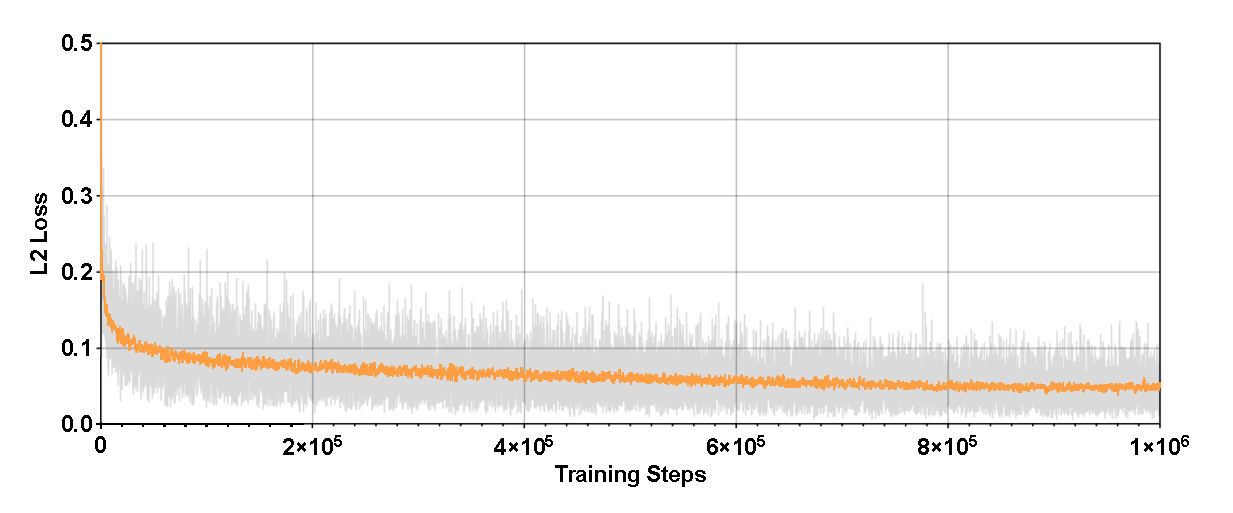
\includegraphics[width=1.\textwidth]{img/diff_loss.eps}
	\caption{L2 loss of the training phase of the diffusion model. Original data (gray) is downsampled and smoothed with a $2^{nd}$ order filter (orange) for visualization. }
	\label{img:diff_loss}
\end{figure}

\section{Evaluation}
\subsection{Evaluation Metrics}
No matter which form of the rotation representation we use during the training phase that is introduced in section \ref{sec:representation}, we transform it back to the rotation matrix $\mathbf{R}$ to evaluate the pose estimation together with the translation, in order to meet the requirement of the data format of \gls{bop}. The pose is represented by a 4x4 matrix $\mathbf{T}=[\mathbf{R},\mathbf{t},\mathbf{0},1]$, where $\mathbf{R}$ is a 3x3 rotation matrix and $\mathbf{t}$ is a 3x1 translation vector. As evaluation metrics, we adopt the same metrics used in \gls{bop} Challenge 2019/2020/2022/2023 \cite{hodan2018bop,hodan2020bop}. The following metrics are used to evaluate the pose estimation. 

\gls{vsd}: 
\begin{align}
 e_{\text{VSD}}\left(\hat{D},\bar{D},\hat{V},\bar{V},\tau\right)=\text{avg}_{p\in \hat{V}\cup \bar{V}}
  \begin{cases}
    0 & \text{if} \ p\in \hat{V}\cap  \bar{V} \land \left|\bar{S}(p)-\hat{S}(p)\right|<\tau\\
    1 & \text{otherwise}
  \end{cases}
\end{align}
An object model is rendered in two poses: the estimated pose $\mathbf{\hat{P}}$ and the ground truth pose $\mathbf{\bar{P}}$. And the result of the rendering is two distance maps $\hat{S}$ and $\bar{S}$. The distance maps are compared with the distance map $S_I$ of the test image to calculate the visibility masks $\hat{V}$ and $\bar{V}$. The error is controlled by a misalignment tolerance $\tau$.

\gls{mssd}:
\begin{align}
  e_{\text{MSSD}}\left(\mathbf{\hat{P}},\mathbf{\bar{P}},S_{M},V_{M}\right)=\min_{\mathbf{S}\in S_{M}}\max_{\mathbf{x}\in V_{M}}\left\Vert \hat{\mathbf{P}}\mathbf{x}-\bar{\mathbf{P}}\mathbf{Sx}\right\Vert _{2} 
 \end{align}
where $S_{M}$ is the set of all symmetry transformations of the object model and $V_{M}$ is the set of model vertices. The \gls{mssd} is the minimum of the maximum symmetric-aware surface distance between the estimated pose $\mathbf{\hat{P}}$ and the ground truth pose $\mathbf{\bar{P}}$. The maximum distance between the model vertices is important for robotic applications, where the maximum surface deviation strongly indicates the chance of a successful grasp.

\gls{mspd}:
\begin{align}
  e_{\text{MSPD}}\left(\mathbf{\hat{P}},\mathbf{\bar{P}},S_{M},V_{M}\right)=\min_{\mathbf{S}\in S_{M}}\max_{\mathbf{x}\in V_{M}}\left\Vert \text{proj}\left(\hat{\mathbf{P}}\mathbf{x}\right)-\text{proj}\left(\bar{\mathbf{P}}\mathbf{Sx}\right)\right\Vert _{2} 
 \end{align}
The proj$(\cdot)$ is the \gls{2d} projection which results in pixels and other variables that are identical to the \gls{mssd}. The \gls{mspd} considers global object symmetries and replaces the average by the maximum distance to increase robustness against the sampling of the object model compared with the previous method \cite{7780735}.

After the error functions are determined, we use the threshold of the error to define the correctness of the pose estimation. The pose is correctly estimated if the error $e<\theta_{e}$, where $e\in \left\{e_{\text{VSD}},e_{\text{MSSD}},e_{\text{MSPD}}\right\}$ and $\theta_{e}$ is the threshold of correctness.

$\text{\gls{avre}}_{\text{VSD}}$ is the average recall rates calculated for the misalignment tolerence $\tau$ from $5\%$ to $50\%$ of the object diameter with a step of $5\%$, and the threshold of correctness $\theta_{\text{VSD}}$ ranging from $0.05$ to $0.5$ with a step of $0.05$. $\text{\gls{avre}}_{\text{MSSD}}$ is the average recall rate calculated for the threshold of correctness $\theta_{\text{MSSD}}$ ranging from $0.05$ to $0.5$ of the object diameter with a step of $0.05$. $\text{\gls{avre}}_{\text{MSPD}}$ is the average recall rate calculated for the threshold of correctness $\theta_{\text{MSPD}}$ ranging from $5r$ to $50r$ with a step of $5r$, where $r=w/640$ and $w$ is the image width in pixels. The average recall rate is defined as:
\begin{align}
  \text{AR}=\left(\text{AR}_{\text{VSD}}+\text{AR}_{\text{MSSD}}+\text{AR}_{\text{MSPD}}\right)/3
\end{align}

The most popular metrics for pose estimation have been the \gls{add} and the \gls{adds} \cite{hinterstoisser2012model}. The \gls{add} is the average distance between the model vertices transformed with the estimated pose and the model vertices transformed with the ground truth pose and the \gls{adds} is the version considering the pose ambiguity of the rotationally symmetric object. \gls{add} and \gls{adds} are defined as:
\begin{gather}
  \text{ADD}=\frac{1}{\left|V\right|}\sum_{\mathbf{x}\in V}\left\Vert \hat{\mathbf{P}}\mathbf{x}-\bar{\mathbf{P}}\mathbf{x}\right\Vert _{2}\\
  \text{ADD-S}=\frac{1}{\left|V\right|}\sum_{\mathbf{x}_{1}\in V}\min_{\mathbf{x}_{2}\in V}\left\Vert \hat{\mathbf{P}}\mathbf{x}_{1}-\bar{\mathbf{P}}\mathbf{x}_{2}\right\Vert _{2}
\end{gather}
where $V$ is the set of model vertices. It has some limitations that \gls{add}(-S) comes from a high dependence on the geometry of the object model and the sampling density of its surface, i.e. the average distance is dominated by higher-frequency surface parts such as the thread of a fuse. The maximum distance used in \gls{mssd} and \gls{mspd} is less dependent on the geometry and sampling of the object model \cite{hodan2020bop}.

\subsection{Pose Estimation Results}
We evaluate our model on the test dataset of \gls{bop} challenge \cite{hodan2018bop} with overall 3000 images and use the segmentation result from the ground truth as our mask to filter out the background, since we only focus on the pose estimation with an object already detected. In this section, we represent both quantitative results and qualitative estimation of given input. Our method is also compared with the state-of-the-art methods on this task.

\subsubsection{Quantitative Evaluation}
Following the metrics that we introduced in the previous section, we propose comprehensive evaluations on each object of both \gls{lm} and \gls{lmo} datasets. The corresponding results of all categories are shown in table \ref{tab:eval_categories_lm} and \ref{tab:eval_categories_lmo}. In figure \ref{img:eval_threshold} we can further validate the capability of our model facing each object with different thresholds of correctness. The object like cup, whose \gls{avre} of \gls{bop} metrics and \gls{add}(-S) is relatively lower, is hard to estimate. This is because of the ambiguity caused by the handle when it is not visible and this identification part only takes a small partition in the whole object. Besides that, our model achieves quite satisfying results even when dealing with the object with occlusion.
\begin{table}[h]
  \centering
  \caption{Quantitative Evaluation on LM dataset(symmetrical objects annotated with $^{*}$).}
  \label{tab:eval_categories_lm}
  \fontsize{11pt}{11pt}\selectfont
  \begin{tabular}{l | C{8mm} C{8mm} C{8mm} C{8mm} C{8mm} C{8mm}| C{8mm} C{8mm}| C{8mm} C{8mm}}
      \toprule
       & \multicolumn{2}{c}{$\text{AR}_{\text{MSPD}}$}  & \multicolumn{2}{c}{$\text{AR}_{\text{MSSD}}$} & \multicolumn{2}{c|}{$\text{AR}_{\text{VSD}}$} & \multicolumn{2}{c|}{AR} & \multicolumn{2}{c}{ADD(-S)} \\
      \midrule
      Refinement & $-$ & $\surd$ & $-$ & $\surd$ & $-$ & $\surd$ & $-$ & $\surd$ & $-$ & $\surd$ \\
      \midrule
      Ape           & 85.6 & 93.9 & 73.9 & 87.6 & 58.7 & 80.4 & 72.7 & 87.3 & 73.5 & 92.0 \\
      Bench vi.     & 78.8 & 87.3 & 85.2 & 89.8 & 61.3 & 74.7 & 75.1 & 83.9 & 93.0 & 93.0 \\
      Bowl$^{*}$    & 80.3 & 83.6 & 77.6 & 82.7 & 42.9 & 60.6 & 66.9 & 75.7 & 99.0 & 99.5 \\
      Camera        & 73.7 & 82.8 & 73.0 & 82.3 & 57.7 & 73.2 & 68.1 & 79.4 & 70.0 & 81.0 \\
      Can           & 73.8 & 83.1 & 76.2 & 84.6 & 54.5 & 71.5 & 68.1 & 79.8 & 82.0 & 86.5 \\
      Cat           & 88.2 & 97.2 & 86.1 & 95.9 & 60.3 & 83.4 & 78.2 & 92.2 & 96.0 & 97.0 \\
      Cup           & 53.7 & 59.5 & 46.9 & 53.8 & 30.0 & 51.2 & 43.5 & 54.8 & 31.5 & 51.5 \\
      Driller       & 78.2 & 85.6 & 87.0 & 92.3 & 60.4 & 77.3 & 75.2 & 85.1 & 95.5 & 95.0 \\
      Duck          & 77.5 & 85.4 & 67.0 & 78.2 & 53.5 & 71.7 & 66.0 & 78.4 & 66.5 & 81.0 \\
      Egg box$^{*}$ & 65.9 & 72.0 & 64.2 & 70.3 & 59.0 & 68.4 & 63.0 & 70.2 & 99.0 & 99.0 \\
      Glue$^{*}$    & 72.6 & 79.8 & 70.1 & 77.6 & 46.0 & 62.3 & 62.9 & 73.2 & 92.0 & 93.0 \\
      Hole pu.      & 68.4 & 73.9 & 62.8 & 69.3 & 38.7 & 49.9 & 56.6 & 64.3 & 53.5 & 67.0 \\
      Iron          & 79.5 & 84.4 & 88.3 & 91.9 & 67.9 & 77.2 & 78.6 & 84.5 & 93.5 & 95.0 \\
      Lamp          & 74.9 & 83.6 & 86.1 & 90.5 & 59.7 & 71.9 & 73.6 & 82.0 & 91.0 & 91.5 \\
      Phone         & 83.7 & 89.2 & 87.0 & 92.3 & 61.5 & 74.7 & 77.4 & 85.4 & 95.0 & 96.0 \\
      \midrule
      Mean          & 75.6 & 82.8 & 75.4 & 82.6 & 54.1 & 69.9 & 68.4 & 78.4 & 82.1 & 87.9 \\
      \bottomrule
  \end{tabular}
\end{table}

\begin{table}[h]
  \centering
  \caption{Quantitative Evaluation on LMO dataset(symmetrical objects annotated with $^{*}$).}
  \label{tab:eval_categories_lmo}
  \fontsize{11pt}{11pt}\selectfont
  \begin{tabular}{l | C{8mm} C{8mm} C{8mm} C{8mm} C{8mm} C{8mm}| C{8mm} C{8mm}| C{8mm} C{8mm}}
      \toprule
       & \multicolumn{2}{c}{$\text{AR}_{\text{MSPD}}$}  & \multicolumn{2}{c}{$\text{AR}_{\text{MSSD}}$} & \multicolumn{2}{c|}{$\text{AR}_{\text{VSD}}$} & \multicolumn{2}{c|}{AR} & \multicolumn{2}{c}{ADD(-S)} \\
      \midrule
      Refinement & $-$ & $\surd$ & $-$ & $\surd$ & $-$ & $\surd$ & $-$ & $\surd$ & $-$ & $\surd$ \\
      \midrule
      Ape           & 68.1 & 75.3 & 56.4 & 66.6 & 43.4 & 54.5 & 56.0 & 65.4 & 54.4 & 76.5 \\
      Can           & 55.4 & 64.3 & 58.0 & 65.6 & 36.3 & 54.2 & 49.9 & 61.4 & 61.0 & 68.7 \\
      Cat           & 55.8 & 59.4 & 50.9 & 54.9 & 33.5 & 43.9 & 46.7 & 52.7 & 75.7 & 88.3 \\
      Driller       & 64.9 & 68.6 & 73.0 & 74.6 & 43.4 & 56.9 & 60.4 & 66.7 & 73.6 & 74.1 \\
      Duck          & 41.3 & 45.7 & 34.6 & 40.7 & 37.7 & 49.6 & 37.9 & 45.3 & 35.8 & 47.0 \\
      Egg box$^{*}$ & 27.9 & 29.8 & 20.5 & 22.4 & 21.8 & 24.2 & 23.4 & 25.5 & 89.8 & 89.8 \\
      Glue$^{*}$    & 51.4 & 57.4 & 52.1 & 57.4 & 32.7 & 43.9 & 45.4 & 52.9 & 88.5 & 89.4 \\
      Hole pu.      & 51.6 & 57.3 & 46.7 & 53.5 & 31.3 & 42.5 & 43.2 & 51.1 & 32.5 & 47.7 \\
      \midrule
      Mean          & 52.1 & 57.2 & 49.0 & 54.5 & 35.0 & 46.2 & 45.4 & 52.6 & 63.9 & 72.7 \\
      \bottomrule
  \end{tabular}
\end{table}



Comparing with other \gls{6dof} pose estimation methods in recent years (table \ref{tab:eval_compare_lm}, \ref{tab:eval_compare_lmo}) including \gls{rgb}-only and \gls{rgbd} approaches, our model owns comparable performance, especially on \gls{lmo} dataset. It is easy to notice the significant \gls{avre} drop between the result on \gls{lm} and \gls{lmo} of some methods, which is even more than $40\%$. Our method however has an acceptable score with and without refinement. Why we only use \gls{add}(-S) as the evaluation metric in this part of the comparison, is because the majority of pose estimation methods only provide \gls{add}(-S) in publications and the result of \gls{bop} metrics are not always available. Our ablation study based on all the metrics of \gls{bop} is shown in the next section.

\begin{table}[h]
  \centering
  \caption{Comparison of ADD(-S) scores with other methods on LM dataset (symmetrical objects annotated with $^{*}$).}
  \label{tab:eval_compare_lm}
  \fontsize{10pt}{10pt}\selectfont
  \begin{tabular}{l | C{12mm} | C{12mm} | C{12mm} | c c | c c | C{12mm} | c c}
      \toprule
      Method & Pix2-Pose \cite{Park_2019} & PVNet \cite{peng_pvnet_2019} & Hybrid-Pose \cite{song2020hybridpose} & \multicolumn{2}{c|}{DPOD \cite{zakharov2019dpod}} & \multicolumn{2}{c|}{DF \cite{wang2019densefusion}} & FFB6D \cite{he2021ffb6d} & \multicolumn{2}{c}{Ours}\\
      \midrule
      Data & \multicolumn{5}{c|}{RGB} & \multicolumn{5}{c}{RGB-D} \\
      \midrule
      Refinement & $\surd$ & $-$ & $\surd$ & $-$ & $\surd$ & $-$ & $\surd$ & $-$ & $-$ & $\surd$ \\
      \midrule
      Ape           & 58.1 & 43.6 & 63.1 & 53.3 & 87.7 & 79.5 & 92.3 & 98.4 & 73.5 & 92.0 \\
      Bench vi.     & 91.0 & 99.9 & 99.9 & 95.3 & 98.5 & 84.2 & 93.2 & 100  & 93.0 & 93.0 \\
      Camera        & 60.9 & 86.9 & 90.4 & 90.4 & 96.1 & 76.5 & 94.4 & 99.9 & 70.0 & 81.0 \\
      Can           & 84.4 & 95.5 & 98.5 & 94.1 & 99.7 & 86.6 & 93.1 & 99.8 & 82.0 & 86.5 \\
      Cat           & 65.0 & 79.3 & 89.4 & 60.4 & 94.7 & 88.8 & 96.5 & 99.9 & 96.0 & 97.0 \\
      Driller       & 76.3 & 96.4 & 98.5 & 97.7 & 98.8 & 77.7 & 87.0 & 100  & 95.5 & 95.0 \\
      Duck          & 43.8 & 52.6 & 65.0 & 66.0 & 86.3 & 76.3 & 92.3 & 98.4 & 66.5 & 81.0 \\
      Egg box$^{*}$ & 96.8 & 99.2 & 100  & 99.7 & 99.9 & 99.9 & 99.8 & 100  & 99.0 & 99.0 \\
      Glue$^{*}$    & 79.4 & 95.7 & 98.8 & 93.8 & 96.8 & 99.4 & 100  & 100  & 92.0 & 93.0 \\
      Hole pu.      & 74.8 & 81.9 & 89.7 & 65.8 & 86.9 & 79.0 & 92.1 & 99.8 & 53.5 & 67.0 \\
      Iron          & 83.4 & 98.9 & 100  & 99.8 & 100  & 92.1 & 97.0 & 99.9 & 93.5 & 95.0 \\
      Lamp          & 82.0 & 99.3 & 99.5 & 88.1 & 96.8 & 92.3 & 95.3 & 99.9 & 91.0 & 91.5 \\
      Phone         & 45.0 & 92.4 & 94.9 & 74.2 & 94.7 & 88.0 & 92.8 & 99.7 & 95.0 & 96.0 \\
      \midrule
      Mean          & 72.4 & 86.3 & 91.3 & 83.0 & 95.2 & 86.2 & 94.3 & 99.7 & 82.1 & 87.9 \\
      \bottomrule
  \end{tabular}
\end{table}

\begin{table}[h]
  \centering
  \caption{Comparison of ADD(-S) scores with other methods on LMO dataset (symmetrical objects annotated with $^{*}$).}
  \label{tab:eval_compare_lmo}
  \fontsize{10pt}{10pt}\selectfont
  \begin{tabular}{l | C{12mm} | C{12mm} | C{12mm} | C{12mm} | C{12mm} | C{12mm} | C{9mm} C{9mm}}
      \toprule
      Method & Pix2-Pose \cite{Park_2019} & PVNet \cite{peng_pvnet_2019} & Hybrid-Pose \cite{song2020hybridpose} & GDR-Net \cite{wang2021gdrnet} & Zebra-Pose \cite{su2022zebrapose} & FFB6D \cite{he2021ffb6d} & \multicolumn{2}{c}{Ours}\\
      \midrule
      Data & \multicolumn{5}{c|}{RGB} & \multicolumn{3}{c}{RGB-D} \\
      \midrule
      Refinement & $\surd$ & $-$ & $\surd$ & $-$ & $\surd$ & $-$ & $-$ & $\surd$ \\
      \midrule
      Ape           & 22.0 & 15.8 & 20.9 & 46.8 & 57.9 & 47.2 & 54.4 & 76.5 \\
      Can           & 44.7 & 63.3 & 75.3 & 90.8 & 95.0 & 85.2 & 61.0 & 68.7 \\
      Cat           & 22.7 & 16.7 & 24.9 & 40.5 & 60.6 & 45.7 & 75.7 & 88.3 \\
      Driller       & 44.7 & 65.7 & 70.2 & 82.6 & 94.8 & 81.4 & 73.6 & 74.1 \\
      Duck          & 15.0 & 25.2 & 27.9 & 46.9 & 64.5 & 53.9 & 35.8 & 47.0 \\
      Egg box$^{*}$ & 25.2 & 50.2 & 52.4 & 54.2 & 70.9 & 70.2 & 89.8 & 89.8 \\
      Glue$^{*}$    & 32.4 & 49.6 & 53.8 & 75.8 & 88.7 & 60.1 & 88.5 & 89.4 \\
      Hole pu.      & 49.5 & 39.7 & 54.2 & 60.1 & 83.0 & 85.9 & 32.5 & 47.7 \\
      \midrule
      Mean          & 32.0 & 40.8 & 47.5 & 62.2 & 76.9 & 66.2 & 63.9 & 72.7 \\
      \bottomrule
  \end{tabular}
\end{table}

It is worth mentioning that our model is not trained on each object separately, so the result can be further improved if we train the model overfitted to each object with the cost of inflexibility. Table \ref{tab:eval_overfit_lmo} shows the difference of the \gls{avre} with a generalized model and an object-specific one evaluating on \gls{lmo}.
\begin{table}[h]
  \centering
  \caption{AR drop between generalized model and overfitted one on LMO dataset.}
  \label{tab:eval_overfit_lmo}
  \begin{tabular}{l | c | C{16mm} C{16mm} C{16mm}| C{16mm}| C{16mm}}
      \toprule
      Method & Refine & $\text{AR}_{\text{MSPD}}$ & $\text{AR}_{\text{MSSD}}$ & $\text{AR}_{\text{VSD}}$ & AR & ADD(-S) \\
      \midrule
      General.   & $-$     & 55.8 & 50.9 & 33.5 & 46.7 & 75.7 \\
      Overfit.   & $-$     & 56.8 & 51.1 & 37.4 & 48.5 & 86.5 \\
      General.   & $\surd$ & 59.4 & 54.9 & 43.9 & 52.7 & 88.3 \\
      Overfit.   & $\surd$ & 61.2 & 56.6 & 46.6 & 54.8 & 93.7 \\
      \bottomrule
  \end{tabular}
\end{table}
\subsubsection{Qualitative Evaluation}
Here we also demonstrate the qualitative result of our model on the pose estimation task by using the visualization toolkit from BOP \cite{hodan2018bop} challenge. Figure \ref{img:eval_vis_img} and \ref{img:vis_all} show some objects from \gls{lm} and \gls{lmo} dataset rendered with the estimated pose on the input image. The first row is the objects without occlusion and the second row is the objects with occlusion. We can observe that the \gls{2d}-projection of the estimated pose has a very high percentage of overlap with the ground truth pose if there is no occlusion. The highlighted estimation and object in the background are shifted a little bit when the visible part of the object is occluded by other objects.
\begin{figure}[h]
	\centering
	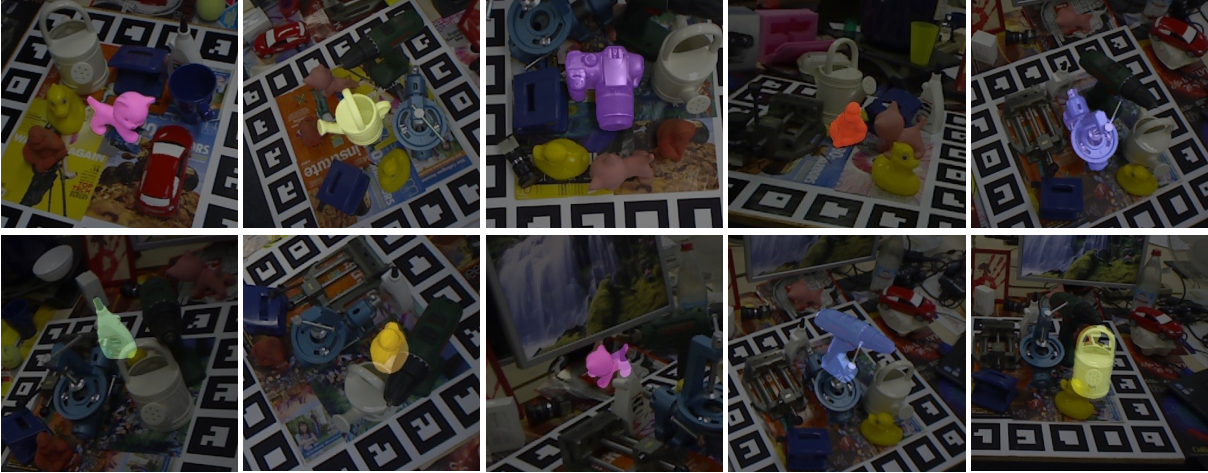
\includegraphics[width=1.\textwidth]{img/eval_vis.pdf}
	\caption{Visualization of some objects highlighted at estimated pose. First row: objects without occlusion; Second row: objects with occlussion.}
	\label{img:eval_vis_img}
\end{figure}

Additionally, we can have a closer look at the development of the pose hypotheses through the whole denoising process (figure \ref{img:eval_vis_denoise}). We select the cat object in \gls{lm} dataset as an example and render the visualization with Blender. The multi-hypotheses (set to 16 in our experiment) of the estimated pose, which is colorized with transparent gray, localize randomly in the space at the early stage of the denoising process and finally overlap together on the ground truth (purple). More examples of the visualization can be found in the appendix \ref{img:vis_cat}, \ref{img:vis_bench}.  
\begin{figure}[h]
	\centering
	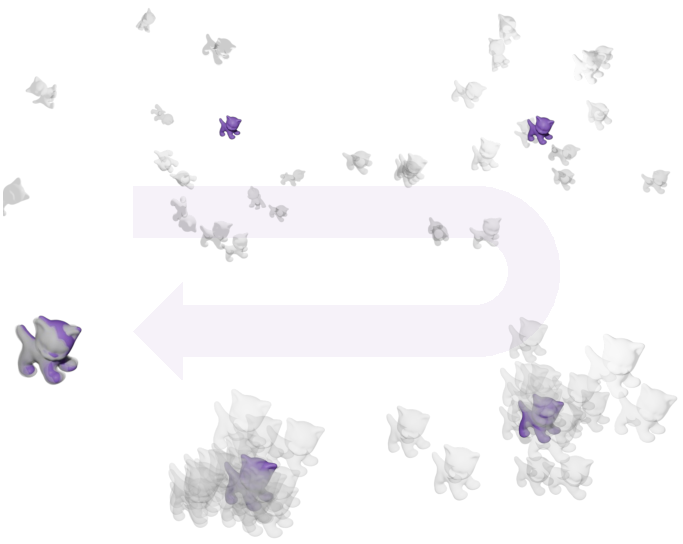
\includegraphics[width=1.\textwidth]{img/vis_denoise.pdf}
	\caption{Visualization of the 6 DoF pose denoising process.}
	\label{img:eval_vis_denoise}
\end{figure}

\section{Ablation Study}
In this section, the ablation study of our method is proposed with the model trained on the \gls{pbr} dataset of one object (cat) to accelerate the training process. We analyze several aspects that influence the performance of the pose estimation. The comparisons are given on both \gls{lm} and \gls{lmo} datasets with and without refinement.
\subsection{Feature Domain}\label{sec:ab_feat}
Here we compare the quantitative results using \gls{2d}, \gls{3d}, and \gls{2d}+\gls{3d} feature given into the backbone since sometimes the ideal \gls{rgbd} data is not available in the real world application. Table \ref{tab:ab_feat_lm} and \ref{tab:ab_feat_lmo} show the evaluation results in different cases. The model utilizing both \gls{2d} and \gls{3d} features achieves naturally the highest score followed by the model only using \gls{3d} feature. \gls{2d}-only method has a relatively wide gap with the other two settings. This is probability because the 2D feature extractor is not trained on the target dataset but on the general image dataset, and the \gls{2d} network suffers from the texture-less object with only limited information available from the data.

However, the additional \gls{2d} information solidly increases the accuracy of the estimation with only \gls{3d} feature. It validates that our feature fusion mechanism doesn't negatively compensate each other, but rather complements the missing information in the other domain.

\begin{table}[h]
  \centering
  \caption{Comparison of the different domains of the feature on LMO dataset.}
  \label{tab:ab_feat_lmo}
  \begin{tabular}{l | c | C{16mm} C{16mm} C{16mm}| C{16mm}| C{16mm}}
      \toprule
      Method & Refine & $\text{AR}_{\text{MSPD}}$ & $\text{AR}_{\text{MSSD}}$ & $\text{AR}_{\text{VSD}}$ & AR & ADD(-S) \\
      \midrule
      2D  & $-$ & 34.7 & 34.4 & 25.5 & 34.6 & 28.8 \\
      3D & $-$ & 54.4 & 49.4 & 33.1 & 45.6 & 78.4 \\
      2D+3D  & $-$ & 56.8 & 51.1 & 37.4 & $\mathbf{48.5}$ & $\mathbf{86.5}$ \\
      2D  & $\surd$ & 52.1 & 43.9 & 36.2 & 44.1 & 56.8 \\
      3D & $\surd$ & 57.4 & 53.5 & 42.2 & 51.0 & 86.5 \\
      2D+3D  & $\surd$ & 61.2 & 56.6 & 46.6 & $\mathbf{54.8}$ & $\mathbf{93.7}$ \\
      \bottomrule
  \end{tabular}
\end{table}

\subsection{Feature Fusion}\label{sec:ab_fusion}
As we introduced in section \ref{sec:fusion}, we run the experiments with entity-wise addition and feature-wise concatenation to evaluate the effect of the different feature fusion. From table \ref{tab:ab_fusion_lm} and \ref{tab:ab_fusion_lmo} we find that the addition of the features outperforms the concatenation in both cases. Normally, the concatenation of the features can preserve more information than the addition with the tradeoff of the larger dimension of the feature. But in our setting, we find that the addition converges fast and performs better than concatenation in the module of feature fusion.

\begin{table}[h]
  \centering
  \caption{Comparison of the different feature fusion methods on LMO dataset.}
  \label{tab:ab_fusion_lmo}
  \begin{tabular}{l | c | C{16mm} C{16mm} C{16mm}| C{16mm}| C{16mm}}
      \toprule
      Method & Refine & $\text{AR}_{\text{MSPD}}$ & $\text{AR}_{\text{MSSD}}$ & $\text{AR}_{\text{VSD}}$ & AR & ADD(-S) \\
      \midrule
      Add  & $-$ & 56.8 & 51.1 & 37.4 & $\mathbf{48.5}$ & $\mathbf{86.5}$ \\
      Concat. & $-$ & 47.0 & 38.2 & 27.3 & 37.5 & 40.5 \\
      Add  & $\surd $ & 61.2 & 56.6 & 46.6 & $\mathbf{54.8}$ & $\mathbf{93.7}$ \\
      Concat. & $\surd $ & 54.6 & 48.0 & 38.5 & 47.1 & 72.1 \\
      \bottomrule
  \end{tabular}
\end{table}

\subsection{Transformation Representation}
Recall the discussion in section \ref{sec:representation} and \ref{sec:res_t}, we compare the different representations of rotation including quaternion, \gls{mrp} and 6D representation \cite{Zhou_2019_CVPR}. From table \ref{tab:ab_rot_lm} and \ref{tab:ab_rot_lmo} we can find that the 6D representation and quaternion have equally best performance on \gls{lm} dataset, and 6D achieves better results on the \gls{lmo} without refinement. Figure \ref{img:ab_rot} shows the convergence of the rotation error with three different forms. We can also see the difference between each representation.

\begin{table}[h]
  \centering
  \caption{Comparison of the different rotation representations on LMO dataset.}
  \label{tab:ab_rot_lmo}
  \begin{tabular}{l | c | C{16mm} C{16mm} C{16mm}| C{16mm}| C{16mm}}
      \toprule
      Method & Refine & $\text{AR}_{\text{MSPD}}$ & $\text{AR}_{\text{MSSD}}$ & $\text{AR}_{\text{VSD}}$ & AR & ADD(-S) \\
      \midrule
      MRP   & $-$     & 55.8 & 50.4 & 35.0 & 47.1 & 83.8 \\
      Quat. & $-$     & 56.1 & 51.0 & 36.4 & 47.8 & 82.0 \\
      6D    & $-$     & 56.8 & 51.1 & 37.4 & $\mathbf{48.5}$ & $\mathbf{86.5}$ \\
      MRP   & $\surd$ & 60.4 & 56.5 & 45.7 & 54.2 & 92.8 \\
      Quat. & $\surd$ & 61.0 & 56.8 & 46.6 & $\mathbf{54.8}$ & $\mathbf{96.4}$ \\
      6D    & $\surd$ & 61.2 & 56.6 & 46.6 & $\mathbf{54.8}$ & 93.7 \\
      \bottomrule
  \end{tabular}
\end{table}

Table \ref{tab:ab_trans_lm} and \ref{tab:ab_trans_lmo} show the results of the model trained with and without residual translation. The advantage of learning the residual error is clear that the \glspl{ar} are improved in both datasets. We can benefit from this trick with respect to the convergence speed shown in figure \ref{img:ab_trans}. The residual translation is also a good way to prevent the model from being trapped in the local minimum.
\begin{table}[h]
  \centering
  \caption{Comparison of the model trained with and without residual translation on LMO dataset.}
  \label{tab:ab_trans_lmo}
  \begin{tabular}{l | c | C{16mm} C{16mm} C{16mm}| C{16mm}| C{16mm}}
      \toprule
      Method & Refine & $\text{AR}_{\text{MSPD}}$ & $\text{AR}_{\text{MSSD}}$ & $\text{AR}_{\text{VSD}}$ & AR & ADD(-S) \\
      \midrule
      w/o res. & $-$     & 57.1 & 50.5 & 28.2 & 45.3 & 69.4 \\
      w/ res.  & $-$     & 56.8 & 51.1 & 37.4 & $\mathbf{48.5}$ & $\mathbf{86.5}$ \\
      w/o res. & $\surd$ & 60.9 & 56.4 & 44.3 & 53.9 & 91.9 \\
      w/ res.  & $\surd$ & 61.2 & 56.6 & 46.6 & $\mathbf{54.8}$ & $\mathbf{93.7}$ \\
      \bottomrule
  \end{tabular}
\end{table}


\subsection{Backbone Scaling}
To test the scaling of our backbone, we compare the results of three different settings of our transformer encoder: Small-L4H2-D128, Base-L8H4-D256 and  Large-L12H6-D768 (L, H and D represent the number of layers, heads and hidden dimensions respectively). The results are shown in table \ref{tab:ab_scale}. With a larger and deeper network, the performance of the diffusion model is improved. The Large setting achieves $1~2\%$ higher \gls{avre} than the Base setting with a tradeoff of additional $20\%$ training time.

\begin{table}[h] 
  \centering
  \caption{Effect of the number of denoising steps on the estimation results.}
  \label{tab:ab_scale}
  \begin{tabular}{l | c | C{12mm} C{12mm} C{12mm}| C{12mm} C{12mm} C{12mm}}
      \toprule
      \multicolumn{2}{c|}{Dataset} & \multicolumn{3}{c|}{LM} & \multicolumn{3}{c}{LMO} \\
      \midrule
      \multicolumn{2}{c|}{\#Steps} & Small & Base & Large & Small & Base & Large \\
      \midrule
      \multirow{2}{*}{AR} & w/o ICP & 66.7 & 68.4 & 69.2 & 44.1 & 45.5 & 47.6 \\
      & w/ ICP & 77.0 & 78.4 & 79.2 & 52.2 & 52.9 & 55.0 \\
      \midrule
      \multirow{2}{*}{ADD(-S)} & w/o ICP & 77.8 & 82.1 & 80.9 & 57.3 & 63.9 & 64.8 \\
      & w/ ICP & 85.9 & 87.9 & 87.8 & 69.4 & 72.7 & 74.2 \\
      \bottomrule
  \end{tabular}
\end{table}

\subsection{Denoising Steps}\label{sec:ab_steps}
In the original \gls{ddpm} setting of the image synthesis task, the diffusion steps are configured as 1000 to ensure the vividness of the generated image. In our pose estimation task, we compare the effects caused by the number of denoising steps on the final result in table \ref{tab:ab_steps}. The result shows that a large number of steps doesn't necessarily lead to better performance. 
\begin{table}[h]
  \centering
  \caption{Effect of the number of denoising steps on the estimation results.}
  \label{tab:ab_steps}
  \begin{tabular}{l | c | C{12mm} C{12mm} C{12mm}| C{12mm} C{12mm} C{12mm}}
      \toprule
      \multicolumn{2}{c|}{Dataset} & \multicolumn{3}{c|}{LM} & \multicolumn{3}{c}{LMO} \\
      \midrule
      \multicolumn{2}{c|}{\#Steps} & 100 & 400 & 1000 & 100 & 400 & 1000 \\
      \midrule
      \multirow{2}{*}{AR} & w/o ICP & 84.0 & 83.2 & 82.8 & 48.3 & 48.5 & 48.5 \\
      & w/ ICP & 94.7 & 94.0 & 93.8 & 54.3 & 54.8 & 54.3 \\
      \midrule
      \multirow{2}{*}{ADD(-S)} & w/o ICP & 98.5 & 97.5 & 98.5 & 89.2 & 86.5 & 85.6 \\
      & w/ ICP & 99.0 & 98.5 & 99.0 & 92.8 & 93.7 & 92.8 \\
      \bottomrule
  \end{tabular}
\end{table}

\chapter{Discussion}
In this chapter, we will discuss our methodology, results from the experiments as well as advantages and drawbacks of our method.

\textbf{Framework} \quad Our approach to \gls{6dof} pose estimation is founded upon the diffusion pipeline, introducing a novel perspective to address this task beyond conventional methods such as direct regression and correspondence matching. By leveraging generative models, specifically the advantageous diversity inherent in diffusion models, our framework enhances the versatility of pose estimation. However, this approach intensifies the intricacy of both training and real-world applications. A pivotal strategy involves segregating the training and inference phases at the network structure level. Inference, due to the iterative nature of the generation process within diffusion models, is inherently intricate and time-consuming.

Despite the incorporation of optimization techniques for sampling, as discussed in Section \ref{sec:impr_sample}, the inference time remains noteworthy compared to more expeditious methods. Notably, the encoder networks, responsible for extracting features from the input data and constituting the diffusion backbone, are trained independently of the diffusion networks. Consequently, our model is not an end-to-end system, necessitating the pretraining of feature extractors through subtasks or the utilization of pre-existing generalized models. This delineation of tasks ensures the effective functioning of the overall framework while acknowledging the intricacies inherent in the training and deployment phases.
\bigbreak
\textbf{Featue Fusion} \quad Within our methodology, we leverage both \gls{2d} and \gls{3d} features from the input data to maximize information extraction. However, the fusion of features across different domains poses a non-trivial challenge in the realm of deep learning. Although we initially explored intuitive methods such as addition and concatenation, these operations are not always the most efficient or effective. The ablation study (refer to Section \ref{sec:ab_fusion}) underscores the substantial impact that the choice of feature fusion methodology has on the final results.

Moreover, our approach involves extracting global features from both the \gls{2d} and \gls{3d} domains to characterize the object within a specific pose. The fusion of global features is relatively straightforward, involving the matching of feature dimensions through the application of projection layers. However, when extracting local features through patchified sampling or dense feature extraction from key points, aligning these local features across different domains becomes a non-trivial task, adding an additional layer of complexity to our methodology.
\bigbreak
\textbf{2D Feature Extractor} \quad In our methodology, we employ a self-supervised \gls{2d} network pre-trained on a comprehensive image dataset to extract \gls{2d} features, rather than training it on the specific target dataset. This choice is motivated by the objective of encoding the image with latent expression, and a general pre-trained model possesses the capability to handle previously unseen \gls{rgb} data in downstream tasks. As observed in Section \ref{sec:ab_feat}, utilizing only \gls{2d} features results in suboptimal performance, particularly in scenarios involving occlusion. While enhancing performance is conceivable through supervised training of the \gls{2d} network specifically for the pose estimation task, this approach deviates from our primary objective. We aim to demonstrate the efficacy of the diffusion framework in processing indistinct input features.

The decision to use a pre-trained network, which has learned representations from a diverse array of images, aligns with the overarching goal of showcasing the adaptability of diffusion models across various applications and datasets. This approach obviates the need to retrain the network from scratch for each new application, providing a more flexible and resource-efficient solution.
\bigbreak
\textbf{3D Feature Extractor} \quad In contrast to \gls{2d} feature extraction networks, there is a notable absence of widely applicable \gls{3d} feature extraction networks that can achieve high accuracy on unseen data for downstream tasks. This scarcity arises from the inherent sparsity of \gls{3d} data, coupled with the point cloud's permutation invariance and its exclusive reliance on geometric information. These factors introduce greater uncertainty into the feature extraction process. Consequently, we opt to train our \gls{3d} network on the target dataset, specifically tailoring it to extract features from a point cloud completion task. As demonstrated in Section \ref{sec:ab_feat}, our chosen approach validates the effectiveness of training a \gls{3d} network for satisfactory results.

It is important to note that the utilized network exhibits commendable performance when dealing with individual objects. However, there remains room for improvement in terms of generalization, particularly in scenarios involving multiple objects. When the occluded portion surpasses a certain percentage of the entire object, the network encounters challenges in accurately completing the shape of the object without prior knowledge. This limitation underscores the need for continued advancements in \gls{3d} feature extraction networks for broader applicability across diverse and complex scenarios.
\bigbreak
\textbf{Diffusion Model} \quad Our diffusion model adopts the architecture of the \gls{ddpm} and incorporates techniques from \gls{ddim} to expedite the inference phase. Visualizations in Figure \ref{img:eval_vis_denoise} demonstrate that, regardless of the initial pose hypothesis, our approach converges to the ground truth pose after a certain number of denoising steps. Notably, the number of denoising steps has a discernible impact on the quality of generated samples in image synthesis tasks. However, as discussed in Section \ref{sec:ab_steps}, in our pose estimation task, varying the number of denoising steps does not significantly alter the results. This can be attributed to the fact that the denoising objective, in terms of transformation, represents a low-dimensional representation of a \gls{3d} object compared to a point cloud. The \gls{2d} image itself is a high-dimensional matrix with more entities (pixels) and channels, necessitating more denoising steps to ensure meaningful representation and quality at both pixel and image levels. In our context, the transformation vector converges more readily to the ground truth pose, requiring fewer denoising steps.

Unlike the original \gls{ddpm}, our adaptation employs a Transformer encoder as the backbone to accommodate the input data format, diverging from the traditional \gls{cnn}-based network. This choice introduces the advantage of leveraging the self-attention mechanism to capture weighted relationships between input tokens. This attribute proves beneficial for potential extensions of our work into pose estimation for sequence inputs, such as video or object tracking. The self-attention mechanism can enhance the model's understanding of temporal relationships between frames, contributing to more robust estimations. The transformer encoder, designed for sequence inputs, aligns well with the nature of such dynamic scenarios.

In our experiments, we adopt the mean of multi-hypotheses as the final output of the generated pose. This approach serves to further minimize errors with the ground truth and expedite model convergence. In cases involving symmetrical objects or ambiguity arising from occlusion, the distribution of pose hypotheses becomes multi-modal rather than a single peak. In such scenarios, it proves advantageous to sample multiple hypotheses and analyze the distribution of poses, particularly in applications like robot grasping, where determining the optimal pose for object manipulation is crucial.

\chapter{Conclusion}
In this last chapter of our thesis, we summarize the work and highlight the contributions of our method in the field of \gls{6dof} pose estimation. Additionally, it gives an outlook on the future work.
\section{Summary}
This thesis introduces a pioneering framework and comprehensive evaluation for \gls{6dof} pose estimation, a crucial task in computer vision with widespread applications in robotics and augmented reality. Traditional methods, including template-based, keypoint-based, and direct regression approaches, exhibit distinct advantages and constraints in various scenarios. In response, our work proposes a diffusion-based framework for \gls{6dof} pose estimation.

Diffusion models, a category of generative models, excel in generating high-quality samples from randomly initialized noise. The thesis begins with a review of classical diffusion models and related improvements. Our designed diffusion model, tailored for pose estimation, employs a Transformer encoder as the backbone. This encoder estimates noise added at each training step, guided by the noisy pose and conditional information from the input data. During the inference phase, the pose undergoes gradual denoising from initial random noise to final estimation through iterative passes of a denoiser, implemented as the Transformer encoder. Additionally, optional multi-hypotheses and \gls{icp} refinement steps further enhance estimation accuracy.

To extract the feature from the input \gls{rgbd} data. A self-supervised \gls{vit} called DINO \cite{caron2021emerging} is utilized for \gls{2d} feature downstream and a point cloud completion task using FoldingNet \cite{yang2018foldingnet} is designed for \gls{3d} feature. After that, we fuse the feature from both domains to become the conditional embedding form the diffusion model.

To validate the performance of our method, we evaluate our method on \gls{lm} \cite{hinterstoisser2012model} dataset and the occlusion version \gls{lmo} \cite{dataV4MUMX2020} dataset with the comparison of other state-of-the-art methods. Results demonstrate comparable performance, even in the presence of occluded objects. Real-world dataset experiments underscore the applicability of the diffusion-based framework in \gls{6dof} pose estimation. A comprehensive ablation study is conducted, analyzing the impact of various components in our method.

As a pioneering work in diffusion-based \gls{6dof} pose estimation on real-world datasets, our approach not only introduces a novel methodology for this task but also highlights the potential of diffusion models beyond image synthesis applications.

\section{Outlook}
In future research, several aspects of our work can be further improved and expanded. In our thesis, we use the architecture of \gls{ddpm} as our diffusion model. The alternative model like \gls{sgm} \cite{song2020generative,song2020improved} can be also applied to our task to avoid the consideration of normalizing constant in likelihood-based models. The sampling techniques like \gls{cas} \cite{jolicoeurmartineau2020adversarial}, \gls{ald} \cite{dockhorn2022scorebased} and \gls{ddss} \cite{watson2022learning} can be an alternative to the \gls{ddim} to accelerate the inference phase.

Furthermore, attention could be directed towards refining the feature extraction process. While we currently utilize a general pre-trained \gls{2d} network, training the network with supervision on the target dataset could lead to further performance improvements. For \gls{3d} features, exploring techniques like contrastive learning may present a novel direction. The generalization of the \gls{3d} downstream network remains a bottleneck for the flexible application of our method. Discovering ways to extract \gls{3d} features from unseen data using a general model could significantly broaden the utility of our approach. Additionally, investigating advanced feature fusion methods, such as cross-attention, could further enhance the understanding of relationships between features from different domains.

Another avenue for extension is adapting our method for object-tracking tasks. Leveraging the transformer encoder as the diffusion backbone could enable understanding not only of the relationship between rotation and translation within a single frame but also the temporal relationships between frames. The use of multi-hypotheses from diffusion models to generate pose distributions, rather than a single solution, would allow for a better understanding of ambiguity in symmetrical objects and facilitate the identification of the optimal pose for tracking objects.



\appendix
\chapter{Additionally: Evaluation Results}
\section{Quantitative Evaluation}
\begin{figure}[H]
	\centering
	\subfloat{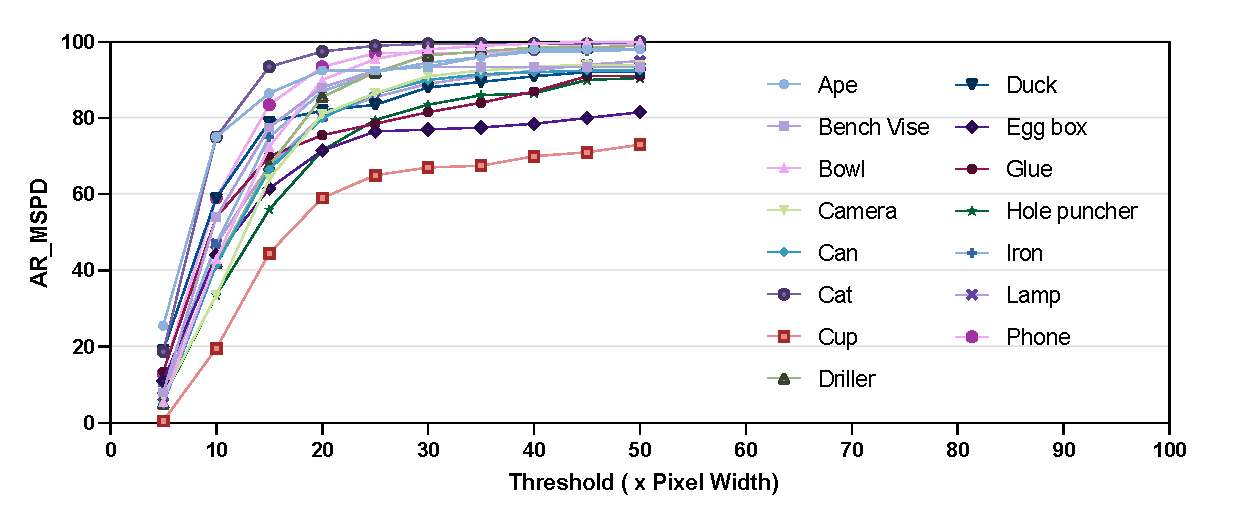
\includegraphics[width=1.\textwidth]{img/mspd_thres.eps}}\\
  \centering
	\subfloat{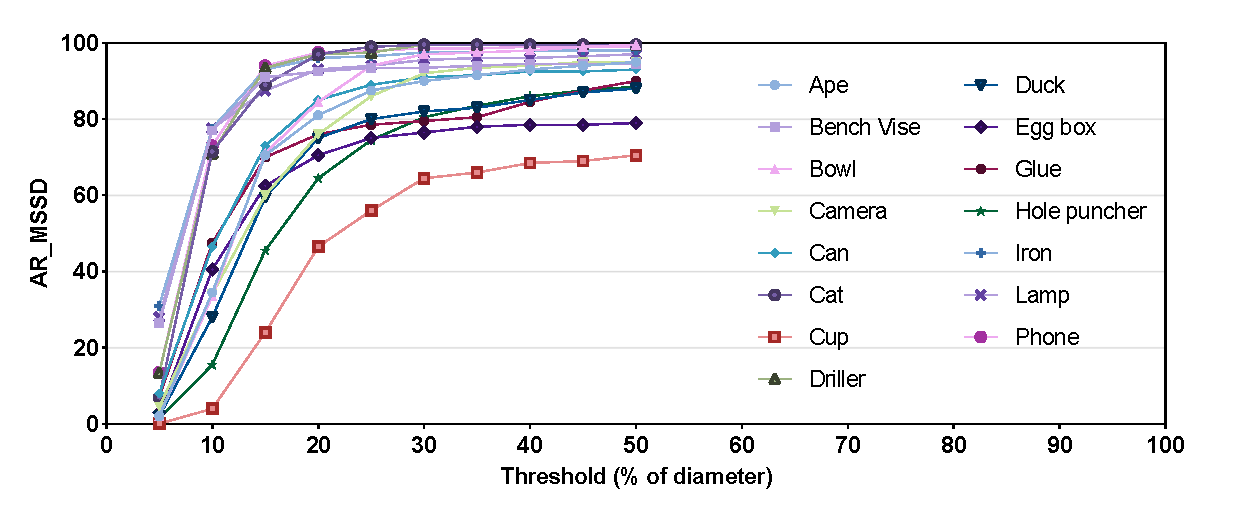
\includegraphics[width=1.\textwidth]{img/mssd_thres.eps}}
	\caption{Categorical MSPD and MSSD recall rates with different thresholds on LM dataset (without refinement).}
	\label{img:eval_threshold}
\end{figure}

\begin{figure}[H]
	\centering
	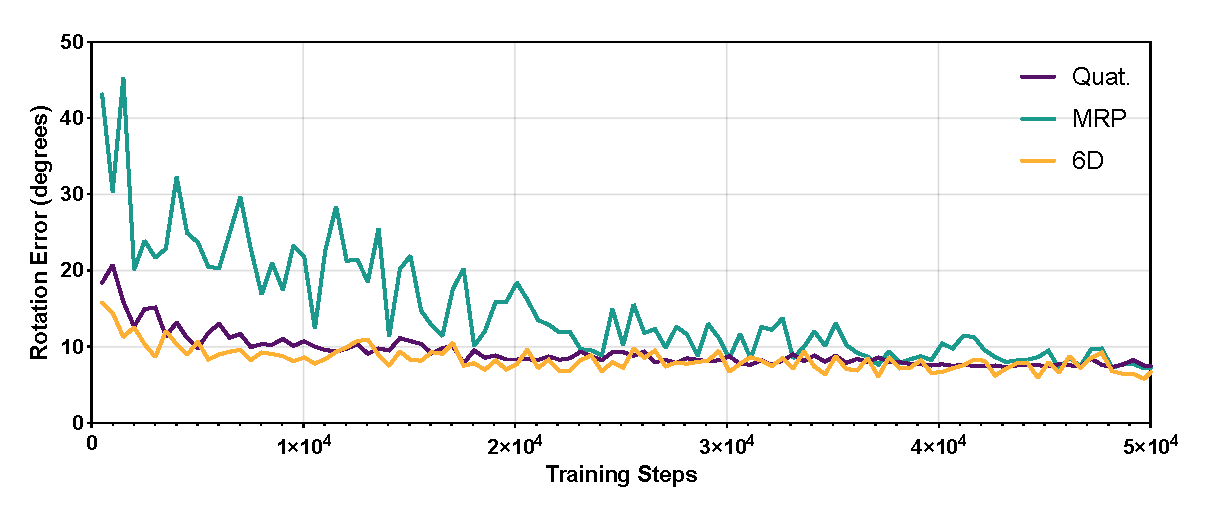
\includegraphics[width=1.\textwidth]{img/ab_rot.eps}
	\caption{Rotation error under different representations of rotation during the training phase (without refinement).}
	\label{img:ab_rot}
\end{figure}

\begin{figure}[H]
	\centering
	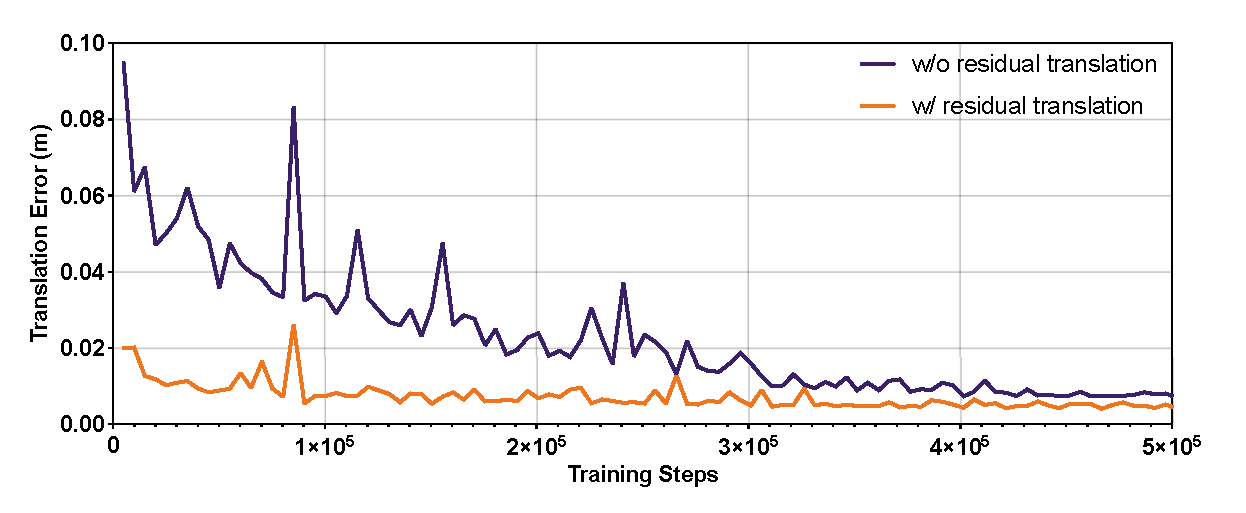
\includegraphics[width=1.\textwidth]{img/ab_trans.eps}
	\caption{Translation error with and without using residual translation during the training phase (without refinement).}
	\label{img:ab_trans}
\end{figure}

\begin{table}[H]
  \centering
  \caption{Comparison of the different domains of the feature on LM dataset.}
  \label{tab:ab_feat_lm}
  \begin{tabular}{l | c | C{16mm} C{16mm} C{16mm}| C{16mm}| C{16mm}}
      \toprule
      Method & Refine & $\text{AR}_{\text{MSPD}}$ & $\text{AR}_{\text{MSSD}}$ & $\text{AR}_{\text{VSD}}$ & AR & ADD(-S) \\
      \midrule
      2D  & $-$ & 77.3 & 73.2 & 47.6 & 66.0 & 76.0 \\
      3D & $-$ & 88.9 & 87.0 & 68.3 & 81.4 & 93.5 \\
      2D+3D  & $-$ & 91.6 & 89.1 & 68.8 & $\mathbf{83.2}$ & $\mathbf{97.5}$ \\
      2D  & $\surd$ & 93.9 & 91.8 & 78.1 & 87.9 & 91.5 \\
      3D & $\surd$ & 94.8 & 93.9 & 83.5 & 90.7 & 95.5 \\
      2D+3D  & $\surd$ & 98.5 & 98.7 & 85.7 & $\mathbf{94.0}$ & $\mathbf{98.5}$ \\
      \bottomrule
  \end{tabular}
\end{table}

\begin{table}[H]
  \centering
  \caption{Comparison of the different feature fusion methods on LM dataset.}
  \label{tab:ab_fusion_lm}
  \begin{tabular}{l | c | C{16mm} C{16mm} C{16mm}| C{16mm}| C{16mm}}
      \toprule
      Method & Refine & $\text{AR}_{\text{MSPD}}$ & $\text{AR}_{\text{MSSD}}$ & $\text{AR}_{\text{VSD}}$ & AR & ADD(-S) \\
      \midrule
      Add  & $-$ & 91.6 & 89.1 & 68.8 & $\mathbf{83.2}$ & $\mathbf{97.5}$ \\
      Concat. & $-$ & 80.9 & 77.5 & 53.2 & 70.5 & 83.5 \\
      Add  & $\surd $ & 98.5 & 98.7 & 85.7 & $\mathbf{94.0}$ & $\mathbf{98.5}$ \\
      Concat. & $\surd $ & 94.8 & 93.7 & 80.4 & 89.7 & 94.0 \\
      \bottomrule
  \end{tabular}
\end{table}

\begin{table}[H]
  \centering
  \caption{Comparison of the different rotation representations on LM dataset.}
  \label{tab:ab_rot_lm}
  \begin{tabular}{l | c | C{16mm} C{16mm} C{16mm}| C{16mm}| C{16mm}}
      \toprule
      Method & Refine & $\text{AR}_{\text{MSPD}}$ & $\text{AR}_{\text{MSSD}}$ & $\text{AR}_{\text{VSD}}$ & AR & ADD(-S) \\
      \midrule
      MRP   & $-$     & 89.4 & 87.0 & 65.2 & 80.5 & 96.0 \\
      Quat. & $-$     & 91.6 & 89.4 & 68.5 & $\mathbf{83.2}$ & $\mathbf{99.0}$ \\
      6D    & $-$     & 91.6 & 89.1 & 68.8 & $\mathbf{83.2}$ & 97.5 \\
      MRP   & $\surd$ & 97.4 & 96.3 & 84.2 & 92.6 & 97.5 \\
      Quat. & $\surd$ & 99.0 & 98.3 & 86.1 & $\mathbf{94.5}$ & $\mathbf{99.0}$ \\
      6D    & $\surd$ & 98.5 & 98.7 & 85.7 & 94.0 & 98.5 \\
      \bottomrule
  \end{tabular}
\end{table}

\begin{table}[H]
  \centering
  \caption{Comparison of the model trained with and without residual translation on LM dataset.}
  \label{tab:ab_trans_lm}
  \begin{tabular}{l | c | C{16mm} C{16mm} C{16mm}| C{16mm}| C{16mm}}
      \toprule
      Method & Refine & $\text{AR}_{\text{MSPD}}$ & $\text{AR}_{\text{MSSD}}$ & $\text{AR}_{\text{VSD}}$ & AR & ADD(-S) \\
      \midrule
      w/o res. & $-$     & 92.0 & 88.3 & 59.3 & 79.9 & 93.5 \\
      w/ res.  & $-$     & 91.6 & 89.1 & 68.8 & $\mathbf{83.2}$ & $\mathbf{97.5}$ \\
      w/o res. & $\surd$ & 98.3 & 97.3 & 84.5 & 93.4 & $\mathbf{99.0}$ \\
      w/ res.  & $\surd$ & 98.5 & 98.7 & 85.7 & $\mathbf{94.0}$ & 98.5 \\
      \bottomrule
  \end{tabular}
\end{table}

\newpage
\section{Qualitative Evaluation}
\begin{figure}[H]
	\centering
	\subfloat{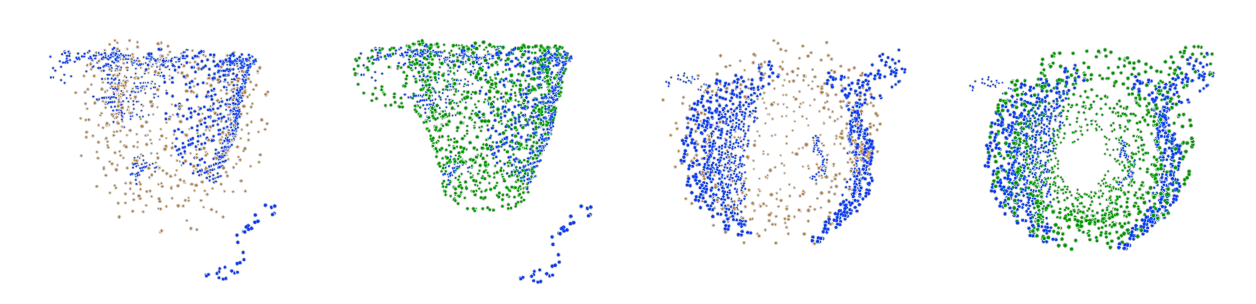
\includegraphics[width=1.\textwidth]{img/comp_cup.pdf}}\\
  \centering
	\subfloat{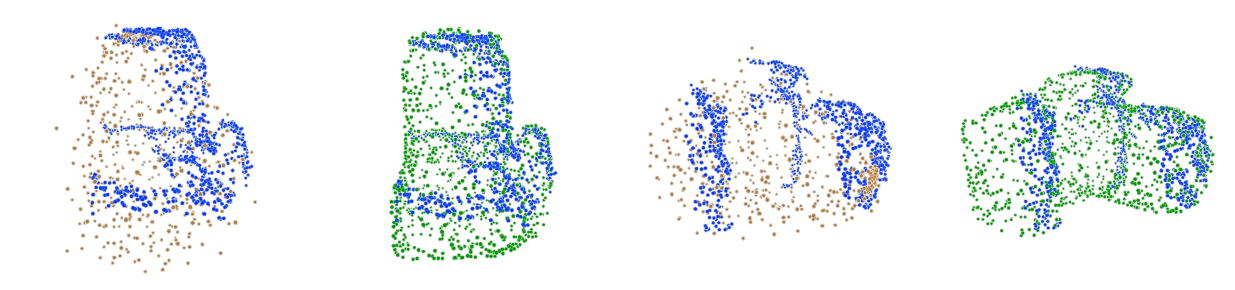
\includegraphics[width=1.\textwidth]{img/comp_cam.pdf}}\\
  \centering
	\subfloat{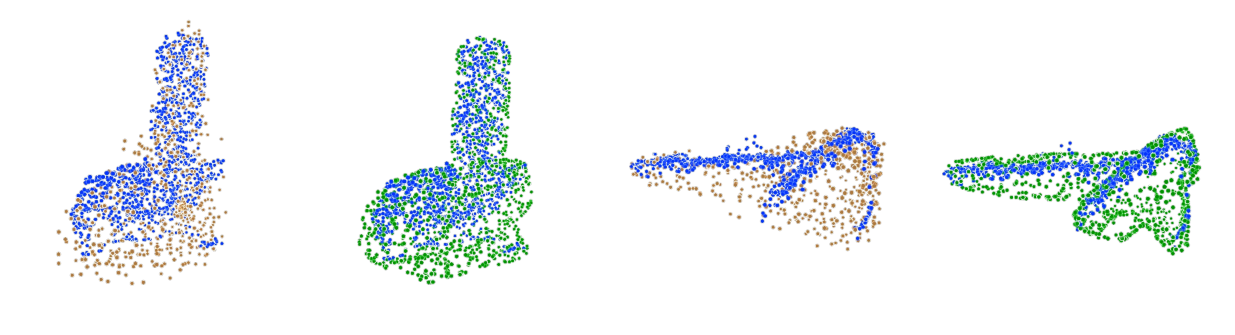
\includegraphics[width=1.\textwidth]{img/comp_phone.pdf}}\\
  \centering
	\subfloat{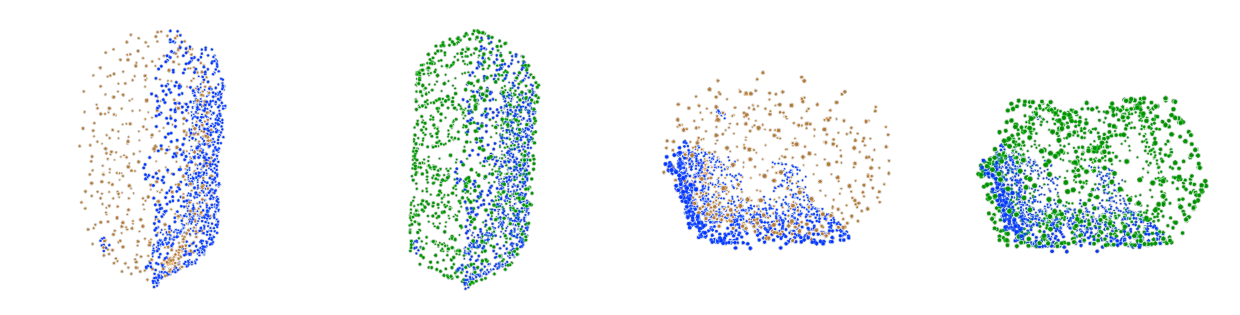
\includegraphics[width=1.\textwidth]{img/comp_egg.pdf}}\\
  \centering
	\subfloat{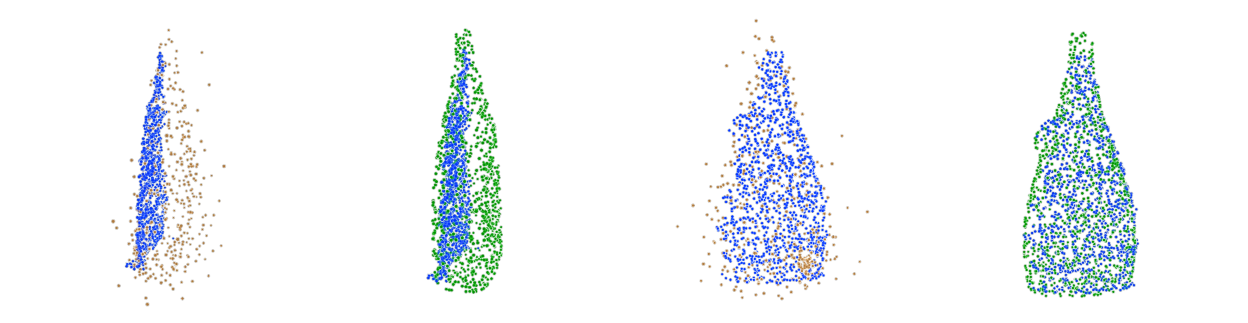
\includegraphics[width=1.\textwidth]{img/comp_glue.pdf}}
	\caption{Point cloud completion results of the FoldingNet. From top to bottom: cup, camera, phone, egg box, glue. From left to right: estimation(viewpoint 1), ground truth(viewpoint 1), estimation(viewpoint 2), ground truth(viewpoint 2). Blue points are the input partial point cloud.}
	\label{img:app_comp}
\end{figure}

\begin{figure}[H]
	\centering
	\includegraphics[width=1.\textwidth]{img/vis_all.pdf}
	\caption{Visualization of some objects highlighted at estimated pose. Row 1-2: objects without occlusion; Row 3-4: objects with occlussion; Row 5: objects with occlusion shown in one scene.}
	\label{img:vis_all}
\end{figure}

\begin{figure}[H]
	\centering
	\includegraphics[width=1.\textwidth]{img/vis_cat.pdf}
	\caption{Visualization of the denoising process of the pose estimation of cat object (Sequence: top to bottom, left to right).}
	\label{img:vis_cat}
\end{figure}

\begin{figure}[H]
	\centering
	\includegraphics[width=1.\textwidth]{img/vis_bench.pdf}
	\caption{Visualization of the denoising process of the pose estimation of bench object (Sequence: top to bottom, left to right).}
	\label{img:vis_bench}
\end{figure}

% -------------------> end writing here <------------------------
% *****************************************************************
\listoffigures
\listoftables

\ifthenelse{\equal{\doclang}{german}}{
	\bibliographystyle{IEEEtran_ISSger}
}{
	\bibliographystyle{IEEEtran_ISS}
}
\bibliography{refs}

% *****************************************************************
%% Additional page with Declaration ("Eidesstattliche Erklrung");
%% completed automatically
\begin{titlepage}
      \vfill
      \LARGE \ifthenelse{\equal{\doclang}{german}}{\textbf{Erkl\"arung}}{\textbf{Declaration}}
      \vfill

      \ifthenelse{\equal{\doclang}{german}}{
         Hiermit erkl\"are ich, dass ich diese Arbeit selbstst\"andig verfasst und keine anderen als die angegebenen
         Quellen und Hilfsmittel benutzt habe.
      }
      {
         Herewith, I declare that I have developed and written the enclosed thesis entirely by myself and that I have not used sources or means except those declared.
      }

      \vspace{1cm}

      \ifthenelse{\equal{\doclang}{german}}{
         Die Arbeit wurde bisher keiner anderen Pr\"ufungsbeh\"orde vorgelegt und auch noch nicht ver\"offentlicht.
      }
      {
         This thesis has not been submitted to any other authority to achieve an academic grading and has not been published elsewhere.
      }

      \vfill

      
      Stuttgart, \signagedate
      \hfill
      \begin{tabular}{l}
          \hline
          \student
      \end{tabular}
\end{titlepage}



\end{document}
